\chapter{การเรียนรู้ของเครื่องและโครงข่ายประสาทเทียม}
\label{chapter: ANN}

\begin{Parallel}[c]{0.45\textwidth}{0.4\textwidth}
	\selectlanguage{english}
	\ParallelLText{
		``If I have seen further, 
		it is by standing upon the shoulders of giants.''
		\begin{flushright}
		---Isaac Newton
		\end{flushright}
	}
	\selectlanguage{thai}
	\ParallelRText{
		``ถ้าผมมองเห็นได้ไกลกว่า  มันก็มาจากการยืนอยู่บนไหล่ของเหล่ายักษ์''
		\begin{flushright}
		---ไอแซค นิวตัน
		\end{flushright}
	}
\end{Parallel}
\index{english}{words of wisdom!Isaac Newton}
\index{english}{quote!build up knowledge}
\vspace{1cm}


วิธี\textit{การเรียนรู้ของเครื่อง}
มีมากมาย หลากหลายแบบ แตกต่างกันไปตามลักษณะงานที่ต้องการ.
ตัวอย่าง \textit{การปรับเส้นโค้งด้วยฟังก์ชันพหุนาม}
ในหัวข้อ~\ref{sec: curve fitting} อภิปรายตัวอย่างง่าย ๆ 
ที่เป็นแนวทางหลัก
และสะท้อนหลักการที่สำคัญของ\textit{การเรียนรู้ของเครื่อง}.
หัวข้อ~\ref{sec: model selection}
%LATER
%และ~\ref{sec: curses of dimensionality}
อภิปรายพื้นฐาน หลักการ และประเด็นสำคัญของศาสตร์\textit{การเรียนรู้ของเครื่อง}. 
%ที่เป็นพื้นฐานกับไม่ว่าจะใช้แบบจำลองเล็ก หรือใหญ่ ไม่ว่าปัญหาธรรมดา หรือปัญหาที่ซับซ้อน ไม่ว่าจะใช้แบบจำลองแบบไหน ใช้โครงข่ายประสาทเทียมหรือไม่ ใช้โครงข่ายประสาทเทียม.
หัวข้อ~\ref{sec: ann}
อภิปราย\textit{โครงข่ายประสาทเทียม}
ซึ่งเป็นแบบจำลองที่สำคัญ ใช้งานได้กว้างขวาง
และเป็นหนึ่งในศาสตร์และศิลป์ของ\textit{การเรียนรู้ของเครื่อง}.
หัวข้อ~\ref{sec: ann applications}
อภิปรายการประยุกต์ใช้งานของ\textit{โครงข่ายประสาทเทียม}.
หัวข้อ~\ref{sec: practical suggestions}
อภิปรายคำแนะนำทั้งสำหรับการใช้งาน\textit{โครงข่ายประสาทเทียม} และการใช้งาน\textit{การเรียนรู้ของเครื่อง}โดยทั่วไป.

\section{การปรับเส้นโค้งด้วยฟังก์ชันพหุนาม}
\label{sec: curve fitting}

\textbf{การทำแบบจำลอง} คือการสร้างสมการคณิตศาสตร์ เพื่อคำนวณค่าคำตอบ $\bm{y}$ จากค่าคำถาม $\bm{x}$.
และหลังจากทำแบบจำลองเสร็จเรียบร้อยแล้ว
แบบจำลองที่ได้ (สมการคณิตศาสตร์ที่นิยามการคำนวณครบทุกอย่างทุกขั้นตอน)
\index{english}{model}
\index{thai}{แบบจำลอง}
จะสามารถนำไปใช้\textit{อนุมาน}หรือ\textit{ทำนาย}ค่าคำตอบ สำหรับคำถามที่สงสัยได้.

พิจารณากรณีที่ทั้งอินพุตและเอาต์พุตเป็นมิติเดียว นั่นคือ คำถาม $x \in \mathbb{R}$
และ $y \in \mathbb{R}$.
หากต้องการจะทำนายค่า $y$ ที่สัมพันธ์กับค่า $x$
โดยที่มีตัวอย่างข้อมูลเป็นคู่ ๆ ของ $(x,y)$
ได้แก่ $(x_1, y_1)$, $(x_2, y_2)$, $\ldots$, $(x_n, y_n)$ %เป็นข้อมูลที่เป็นคู่ ๆ ของค่าที่สนใจ $x$ และ $y$ 
ทั้งหมดจำนวน $n$ คู่.
ตัวแปรต้น $x$ เป็นค่าที่ถามมา
เพื่อหา $y$ ที่เป็นตัวแปรตาม หรือค่าที่อยากได้คำตอบไป.
แต่ละคู่ $(x_i, y_i)$ อาจเรียกว่า \textbf{จุดข้อมูล} (datapoint).
\index{thai}{จุดข้อมูล}
\index{english}{datapoint}

รูป~\ref{fig: curve fitting 10 datapoints}
แสดงตัวอย่างจุดข้อมูล $10$ จุด.
ตำแหน่งของแต่ละ\textit{จุดข้อมูล}ในภาพ
ระบุจากค่า $x$ ตามแกนนอน
และค่า $y$ ตามแกนตั้ง.
ตัวแปรต้น $x$ อาจเรียก \textit{อินพุต} หรือ\textit{ข้อมูลนำเข้า} (input)
และตัวแปรตาม $y$ อาจเรียก \textit{เอาต์พุต} หรือ\textit{ข้อมูลนำออก} (output).
\index{english}{input}
\index{english}{output}
\index{thai}{อินพุต}
\index{thai}{เอาต์พุต}
\index{thai}{ข้อมูลนำเข้า}
\index{thai}{ข้อมูลนำออก}
จากตัวอย่างในภาพ จุดข้อมูลแรกสุด มีค่า $x = 0$ ค่า $y = 0.16$.

เป้าหมายของตัวอย่างนี้คือ การทำนายค่าประมาณเอาท์พุต $y$ ของค่าอินพุต $x$ ที่สงสัย 
โดยอินพุต $x$ อาจจะเป็นค่าเดิม หรืออาจจะเป็นค่าใหม่ที่ไม่เคยเห็นมาก่อน.
%
แนวทางคือ การใช้แบบจำลอง ซึ่งเป็นการคำนวณทางคณิตศาสตร์ ที่เป็นฟังก์ชันของตัวแปร $x$ และใช้ค่าที่ฟังก์ชันคำนวณได้ ทายเป็นค่า $y$.
\index{english}{model}
\index{thai}{แบบจำลอง}
แบบจำลองที่จะเลือกใช้สำหรับตัวอย่างนี้ คือ \textbf{ฟังก์ชันพหุนาม} (polynomial function).
\index{english}{polynomial function}
\index{thai}{ฟังก์ชันพหุนาม}
\textit{ฟังก์ชันพหุนาม} $f$
คำนวณค่า $y$ จาก $x$ โดย
\begin{eqnarray}
y &=& f(x, \bm{w}) = w_0 + w_1 \cdot x + w_2 \cdot x^2 + w_3 \cdot x^3 + \ldots + w_m \cdot x^m
\label{eq: polynomial}
\end{eqnarray}
เมื่อ $\bm{w} = [w_0, \; w_1 \; w_2, \; \ldots, w_m]^T$ เป็นค่า\textit{พารามิเตอร์}ของ\textit{ฟังก์ชันพหุนาม} และ $m$ เป็น\textbf{ระดับขั้น} (degree) ของ\textit{ฟังก์ชันพหุนาม}.
ก่อนที่จะสามารถนำ\textit{ฟังก์ชันพหุนาม}
ไปใช้ทำนายค่า $y$ จากค่า $x$ ที่ถามได้
ต้องกำหนด\textit{ระดับขั้น} $m$
และค่าของ\textit{พารามิเตอร์} $\bm{w}$ ให้เรียบร้อยก่อน.

ตัวอย่างเช่น
หากเลือก
\textit{ระดับขั้น} $m = 2$
และค่าของ\textit{พารามิเตอร์} $\bm{w} = [0.7, -0.65, 1]^T$
สำหรับแบบจำลอง $f_1$ 
นั่นคือ \textit{ฟังก์ชันพหุนาม} $y = f_1(x) = 0.7 -0.65 x + x^2$
แล้วที่ $x = 0.5$
จะทำนายค่า $y$ เป็น $0.625$. 
\textit{ระดับขั้น} 
และค่าของ\textit{พารามิเตอร์}ที่เลือกใช้
ส่งผลโดยตรงกับค่าที่ทำนาย
เช่น
หากเลือก
\textit{ระดับขั้น} $m = 3$
และค่าของ\textit{พารามิเตอร์} $\bm{w} = [0, 13, -39, 32]^T$
สำหรับแบบจำลอง $f_2$
นั่นคือ \textit{ฟังก์ชันพหุนาม} $y = f_2(x) = 13 x -39 x^2 + 32 x^3$
แล้วที่ $x = 0.5$
จะทำนายค่า $y$ เป็น $0.75$ 
ซึ่งแตกต่างจากผลทำนายจาก $f_1$.

%
\begin{figure}[H]
	\begin{center}
		\includegraphics[width=2.0in]
		{03Ann/curvefit/datapoints.png}
	\end{center}
	\caption[ตัวอย่างจุดข้อมูล]{ตัวอย่างจุดข้อมูล $(0, 0.160)$,
		$(0.111, 0.724)$,
		$(0.222, 0.931)$,
		$(0.333, 0.712)$,
		$(0.444, 0.610)$,
		$(0.556, -0.460)$,
		$(0.667, -0.684)$,
		$(0.778, -1.299)$,
		$(0.889, -1.147)$,
		และ $(1, -0.045)$ รวม $10$ จุด.}
	\label{fig: curve fitting 10 datapoints}
\end{figure}
%


\textit{ระดับขั้น}และค่า\textit{พารามิเตอร์}ต่าง ๆ
จะให้ผลการทำนายต่างกัน.
รูป~\ref{fig: polynomial different params} แสดงพฤติกรรมการทำนาย
ของฟังก์ชันพหุนาม
เมื่อเลือกใช้\textit{ระดับขั้น}และค่า\textit{พารามิเตอร์}ต่าง ๆ.
\textit{พฤติกรรมการทำนาย}
หมายถึง
ความสัมพันธ์ระหว่างอินพุตกับเอาต์พุต.
\textit{การปรับเส้นโค้ง}
ใช้ประโยชน์จากการที่
พฤติกรรมการทำนายเปลี่ยนตาม\textit{ระดับขั้น}และค่า\textit{พารามิเตอร์}.
ดังนั้น 
\textit{การปรับเส้นโค้ง}
ทำได้โดยปรับ\textit{ระดับขั้น}
และค่า\textit{พารามิเตอร์}ของสมการ
เพื่อปรับเส้นโค้งให้ได้ผลการทำนายที่ดีขึ้น.

ระดับขั้นของสมการพหุุนาม
จะกำหนดจำนวนพารามิเตอร์ของฟังก์ชันพหุนาม.
การเลือกระดับขั้น เป็นการเลือกความสามารถของแบบจำลองโดยรวม.
ระดับขั้นสูง แบบจำลองจะมีความสามารถมาก
แต่ก็เพิ่มจำนวนพารามิเตอร์ที่ต้องหาค่า เท่ากับ เพิ่มความยากในการปรับแบบจำลองขึ้น.
หัวข้อ~\ref{sec: model selection} 
อภิปรายวิธีการเลือกระดับขั้น.
ตอนนี้ สมมติว่าระดับขั้น $m$ ถูกเลือกมาแล้ว
หากเลือกระดับขั้นเป็น $m$
ฟังก์ชันพหุนามจะมีจำนวนพารามิเตอร์ เป็น $m+1$ ตัว.
การหาค่าของพารามิเตอร์เหล่านี้ จะเรียกว่า \textbf{การฝึก} (training) หรือ \textbf{การเรียนรู้} (learning).
\index{english}{training}
\index{english}{learning}
\index{thai}{การฝึก}
\index{thai}{การเรียนรู้}

%
\begin{figure}[H]
	\begin{center}
		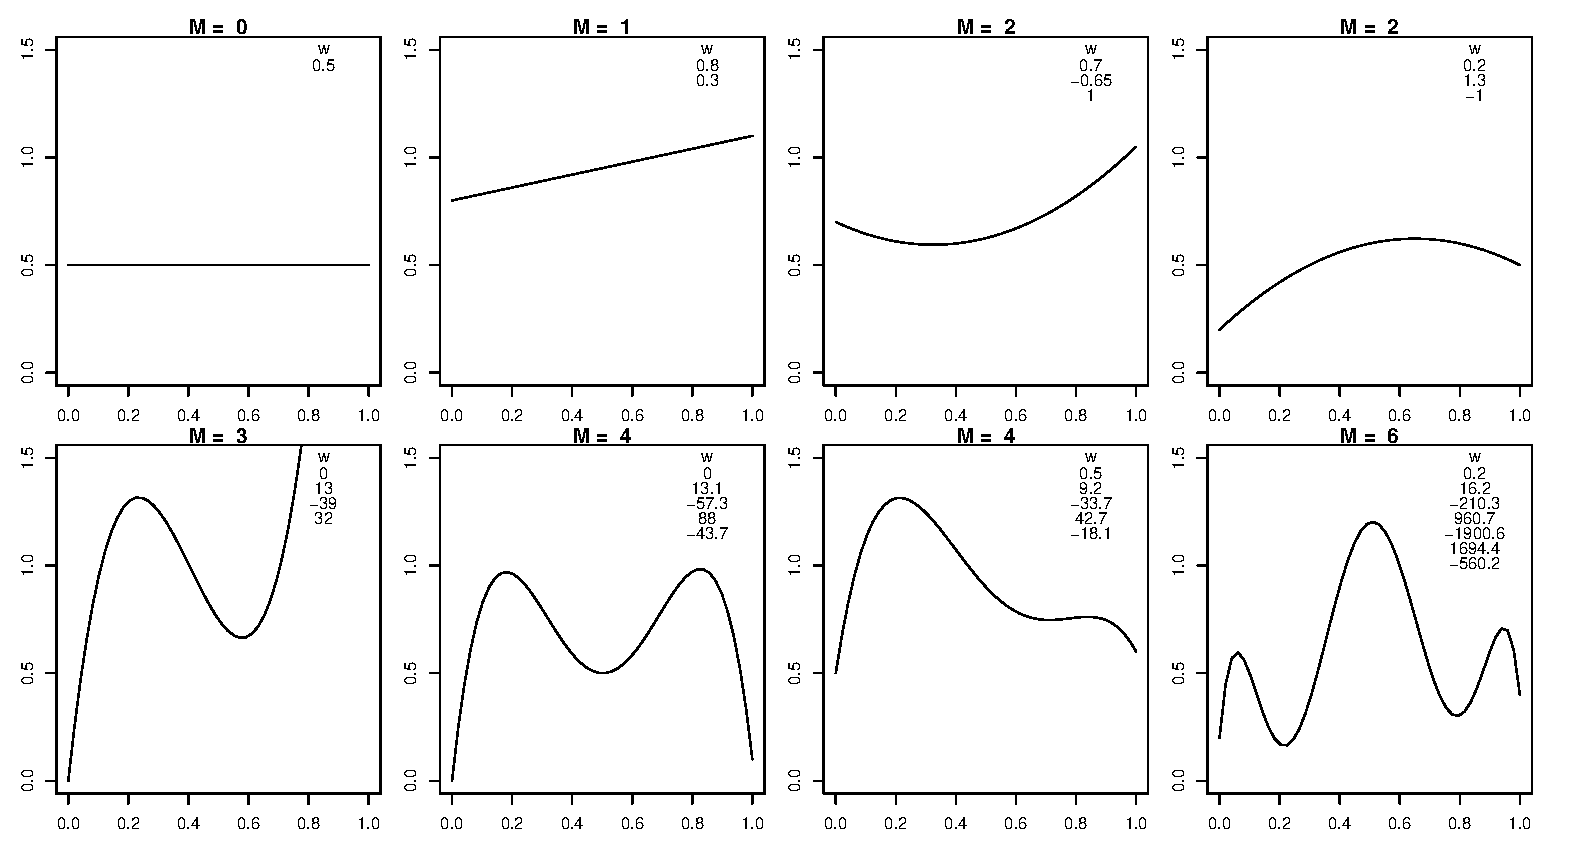
\includegraphics[width=\textwidth]
		{03Ann/curvefit/bgPolynomial.png}
	\end{center}
	\caption[ฟังก์ชันพหุนามต่าง ๆ]{ฟังก์ชันพหุนาม เมื่อเลือกใช้\textit{ระดับขั้น}และค่า\textit{พารามิเตอร์}ต่าง ๆ. \textit{ระดับขั้น} \texttt{M} แสดงเหนือแต่ละภาพ และค่า\textit{พารามิเตอร์} แสดงภายในแต่ละภาพ.}
	\label{fig: polynomial different params}
\end{figure}
%

\paragraph{การฝึกแบบจำลอง.}
\textit{การฝึกแบบจำลอง}
คือการหาค่าพารามิเตอร์ของแบบจำลอง
เพื่อให้แบบจำลองทำนายได้ถูกต้องมากที่สุด
หรือกล่าวอีกอย่างคือ
เพื่อให้แบบจำลองทำนายผิดน้อยที่สุด.
การวัดว่าแบบจำลองทำนายได้ผิดมากน้อยเท่าใด
สามารถใช้แนวทางของ\textbf{วิธีกำลังสองน้อยที่สุด} (Least Square method) ได้.
\textit{วิธีกำลังสองน้อยที่สุด} 
วัดว่าแบบจำลองทำนายได้ผิดมากน้อยเท่าใด
จาก ผลต่างกำลังสอง ระหว่างค่าเอาต์พุตที่ทำนายกับค่าเอาต์พุตจริง.
นั่นคือ $E_n = (\hat{y}_n - y_n)^2$
เมื่อ $E_n$ คือ\textbf{ความผิดพลาด} (error) ของการทำนาย\textit{จุดข้อมูล}ที่ $n^{th}$
ซึ่งวัดจากผลต่างกำลังสองระหว่าง
ค่าเอาต์พุตที่ทำนาย $\hat{y}_n$
สำหรับ\textit{จุดข้อมูล}ที่ $n^{th}$
และค่าเอาต์พุตจริง $y_n$
ของ\textit{จุดข้อมูล}ที่ $n^{th}$.
ค่า $y_n$ ที่ได้จากข้อมูล อาจเรียกว่า \textbf{เอาต์พุตจริง} (ground truth) หรือ \textbf{ค่าเฉลย}.
\index{english}{ground truth}
\index{thai}{ค่าเฉลย}
\index{thai}{เอาต์พุตจริง}
รูป~\ref{fig: square errors}
แสดงผลต่างระหว่างค่าที่ทำนายและค่าเอาต์พุตจริง.
ความผิดพลาดรวม สามารถคำนวณได้ดังสมการ~\ref{eq: SSE}.
%
\begin{eqnarray}
E &=& \frac{1}{2} \sum_{n=1}^N  E_n = \frac{1}{2} \sum_{n=1}^N  (\hat{y}_n - y_n)^2
\label{eq: SSE} .
\end{eqnarray}
%
การยกกำลังสอง
ช่วยให้ความผิดพลาดจากการทายขาดไม่ไปหักล้างกับความผิดพลาดจากการทายเกิน. 
ค่าคงที่ $\frac{1}{2}$ ถูกใช้เพื่อความสะดวก 
(ที่จะได้เห็นต่อไป เมื่อทำการหาอนุพันธ์).

ด้วยวิธีวัดความผิดพลาดนี้ การฝึกฟังก์ชันพหุนามระดับขั้น $m$ ก็สามารถทำได้โดย
$\bm{w}^\ast = \arg\min_{\bm{w}} E$.
เมื่อจบการฝึกแล้ว 
ค่าพารามิเตอร์
$\bm{w}^\ast$
จะถูกนำไปใช้กับฟังก์ชันพหุนามเพื่อทำนาย.
ฟังก์ชันพร้อมด้วยค่าพารามิเตอร์ที่ได้จากการฝึก มักจะเรียกรวม ๆ ว่า \textit{แบบจำลองที่ฝึกแล้ว}.

%
\begin{figure}[H]
	\begin{center}
		\includegraphics[width=0.5\textwidth]
		{03Ann/curvefit/errors.png}
	\end{center}
	\caption[ความผิดพลาดของการทำนาย]{ความผิดพลาดของการทำนายที่จุดข้อมูลต่าง ๆ. จุดดาวสีแดง แสดงจุดข้อมูล. 
	เส้นทึบสีฟ้า แทนพฤติกรรมทำนายจากแบบจำลอง.
ความผิดพลาดวัดจากที่ค่า $x$ เดียวกัน ค่าที่แบบจำลองทำนายห่างจากค่า $y$ ของจุดข้อมูลเท่าไร ในภาพ เน้นความห่างนี้ด้วยเส้นประสีเขียว.}
	\label{fig: square errors}
\end{figure}
%

\paragraph{ตัวอย่างการฝึกแบบจำลองพหุนามระดับขั้นหนึ่ง.}
สำหรับตัวอย่างข้อมูลในรูป~\ref{fig: curve fitting 10 datapoints}
สมมติระดับขั้นที่เลือกคือ ระดับขั้นหนึ่ง ($m=1$)
นั่นคือ $\hat{y} = w_0 + w_1 x$.
ในการฝึกแบบจำลอง ซึ่งคือการหา $w_0$ และ $w_1$ ที่ทำนายผิดพลาดน้อยที่สุด
นั่นคือ การหา $w_0^\ast, w_1^\ast = \arg\min_{w_0, w_1} E$
เมื่อ $E = \frac{1}{2} \sum_{n=1}^N  E_n$
และ
$E_n =  (w_0 + w_1 x_n - y_n)^2$.

ค่าความผิดพลาดต่ำสุด เกิดเมื่อ $\frac{\partial E}{\partial w_0} = 0$ 
และ
$\frac{\partial E}{\partial w_1} = 0$ ซึ่งเมื่อเขียน $E$ ในรูปฟังก์ชันของ $w_0$ และ $w_1$ จะได้
\begin{eqnarray}
\frac{\partial \frac{1}{2} \sum_{n=1}^N \{ w_0 + w_1 x_n - y_n \}^2}{\partial w_0} &=& 0, 
\label{eq: polynomial derivatives 2a}
\\
\frac{\partial \frac{1}{2} \sum_{n=1}^N \{ w_0 + w_1 x_n - y_n \}^2}{\partial w_1} &=& 0
\label{eq: polynomial derivatives 2b}
\end{eqnarray}
และหลังจากหาอนุพันธ์เสร็จจะได้
\begin{eqnarray}
\sum_{n=1}^N \{ (w_0 + w_1 x_n - y_n) \cdot (1 + 0 - 0) \} &=& 0, 
\label{eq: polynomial derivatives 3a} \\
\sum_{n=1}^N \{ (w_0 + w_1 x_n - y_n) \cdot (0 + x_n - 0) \} &=& 0.
\label{eq: polynomial derivatives 3b}
\end{eqnarray}

ทำการจัดรูปใหม่ โดยเรียงตามพารามิเตอร์ จะได้
\begin{eqnarray}
%
w_0 \sum_{n=1}^N \{ 1 \} + w_1 \sum_{n=1}^N \{ x_n \} - \sum_{n=1}^N \{ y_n \} &=& 0, 
\label{eq: poly 4a} \\
w_0 \sum_{n=1}^N \{ x_n \} + w_1 \sum_{n=1}^N \{ x_n^2 \} - \sum_{n=1}^N \{ y_n \cdot x_n \} &=& 0 
\label{eq: poly 4b}
\end{eqnarray}
ซึ่งเมื่อจัดรูปสมการ~\ref{eq: poly 4a} และ~\ref{eq: poly 4b} ให้อยู่ในรูปเมทริกซ์จะได้
\begin{eqnarray}
%
\left[ 
\begin{matrix}
N & \sum_{n=1}^N x_n \\
\sum_{n=1}^N x_n & \sum_{n=1}^N x_n^2
\end{matrix}
\right] \cdot 
\left[ 
\begin{matrix}
w_0 \\
w_1
\end{matrix}
\right]
=
\left[ 
\begin{matrix}
\sum_{n=1}^N y_n \\
\sum_{n=1}^N y_n \cdot x_n
\end{matrix}
\right].
\label{eq: polynomial M1}
\end{eqnarray}

เมื่อนำค่าจุดข้อมูลในรูป~\ref{fig: curve fitting 10 datapoints} มาคำนวณ
ผลจะได้ว่า $N = 10$, $\sum_{n=1}^N x_n = 5$, $\sum_{n=1}^N x_n^2 = 3.519$, $\sum_{n=1}^N y_n = -0.498$, และ $\sum_{n=1}^N y_n x_n = -1.992$.
เมื่อแก้สมการแล้วจะได้ค่า 
$[w_0, \; w_1]^T $ $= [0.805, \; -1.710]^T$.
นั่นคือ แบบจำลอง $\hat{y} = 0.805 - 1.71 x$
พฤติกรรมของแบบจำลองนี้แสดงดังในรูป~\ref{fig: deg-1 polynomial fitting}.

การใช้งาน หรือการทำนายด้วยแบบจำลอง $\hat{y} = 0.805 - 1.71 x$
คือ การคำนวณโดยแทนค่า $x$ ที่ถามลงไป
เช่น ที่ $x = 0.5$ แบบจำลองนี้ทำนาย
$\hat{y} = 0.805 - 1.71 (0.5)$
$=-0.05$.
ความสามารถของแบบจำลองนี้
ประเมินคราว ๆ ได้จาก\textit{ค่าความผิดพลาดรวม} (สมการ~\ref{eq: SSE}) $E = 1.487$. 


%
\begin{figure}[H]
	\begin{center}
		\includegraphics[width=0.5\textwidth]
		{03Ann/curvefit/Degree1Fitting.png}
	\end{center}
	\caption[พหุนามระดับขั้นหนึ่งที่ฝึกแล้ว]{พฤติกรรมของแบบจำลองพหุนามระดับขั้นหนึ่งที่ฝึกแล้ว (เส้นทึบสีฟ้า) กับจุดข้อมูลที่ฝึก (ดาวสีแดง).}
	\label{fig: deg-1 polynomial fitting}
\end{figure}
%

{\small
	\begin{shaded}
		\paragraph{\small เกร็ดความรู้สมองมนุษย์}
		(เรียบเรียงจาก \cite{NIND} \cite{BuddhasBrain} และ \cite{Wikipedia})
		\index{thai}{สมองมนุษย์}
		\index{english}{Human Brain}
		\index{english}{side story}
		\index{english}{side story!Human Brain}
		\index{thai}{เกร็ดความรู้}
		\index{thai}{เกร็ด!สมองมนุษย์}
		
		โดยเฉลี่ยแล้ว สมองมนุษย์มีขนาดประมาณ $1.13$ ถึง $1.26$ ลิตร และหนักประมาณ $1.3$ กก.
		ใช้ออกซิเจนประมาณ $20$ เปอร์เซ็นของปริมาณทั้งหมดที่ร่างกายรับเข้าไป
		และใช้กำลังงานประมาณ $25$ วัตต์\cite{GodwinCham2012a}.
		%
		
		สมองเชื่อมต่อกับส่วนอื่น ๆ ของร่างกายผ่านไขสันหลัง 
		%(สมองและไขสันหลังประกอบกันเป็น\textit{ระบบประสาทกลาง} (Central Nervous System คำย่อ CNS) 
		และ\textit{ระบบประสาทนอกส่วนกลาง} (Peripheral Nervous System คำย่อ PNS) 
		%
		%และ\textit{ไขสันหลัง} (Spinal Cord)ประกอบกันเป็น\textit{ระบบประสาทกลาง} (Central Nervous System คำย่อ CNS).
		ไขสันหลังทำหน้าที่หลัก ๆ คือเชื่อมต่อสัญญาณควบคุมจากสมองไปยังส่วนต่าง ๆ ของร่างกาย และส่งผ่านสัญญาณรับรู้จากส่วนต่าง ๆ ของร่างกายกลับไปยังสมอง
		และไขสันหลังเองก็มีระบบประสาทของตัวเองที่ช่วยทำงาน เช่น การควบคุมการตอบสนองฉับพลัน.
		ระบบประสาทนอกส่วนกลาง มีหน้าที่หลัก
		คือเชื่อมต่อสัญญาณจากสมองและไขสันหลังไปสู่อวัยวะต่าง ๆ.
		%
		%The spinal cord functions primarily in the transmission of neural signals between the brain and the rest of the body but also contains neural circuits that can independently control numerous reflexes and central pattern generators. The spinal cord has three major functions: as a conduit for motor information, which travels down the spinal cord, as a conduit for sensory information in the reverse direction, and finally as a center for coordinating certain reflexes.
		
		การทำงานของสมองมีลักษณะคล้ายคณะกรรมการของกลุ่มผู้เชี่ยวชาญจำนวนมาก
		นั่นคือ ส่วนต่าง ๆ ของสมองทำงานร่วมกัน แต่ว่าแต่ละส่วนของสมองมีหน้าที่เฉพาะด้าน.
		เราอาจมองได้ว่าส่วนของสมองมีสามส่วนใหญ่ ๆ คือ \textit{สมองส่วนบน} (forebrain), \textit{สมองส่วนกลาง} (midbrain), และ \textit{สมองส่วนล่าง} (hindbrain).
		
		สมองส่วนล่างนับรวมส่วนบนของไขสันหลัง \textit{ก้านสมอง} (brain stem) และ \textit{เซเรเบลัม} (cerebellum).
		สมองส่วนล่างจะควบคุมการทำงานที่เป็นพื้นฐานของการดำรงชีพ เช่น การหายใจ และการเต้นของหัวใจ.
		เซเรเบลัมช่วยประสานงานเรื่องการเคลื่อนไหวและการเรียนรู้ของการเคลื่อนไหวที่เกิดจากการฝึกทำซ้ำ ๆ เช่น 
		การเล่นเปียโนหรือการตีลูกเทนนิส จะอาศัยการทำงานของเซเรเบลัมช่วย.
		%การฝึกการเคลื่อนไหวของศิลปะการต่อสู้ ที่ฝึกกระบวนท่าต่าง ๆ ซ้ำ ๆ บ่อย ๆ จนเกิดความชำนาญ
		
		สมองส่วนกลางอยู่ด้านบนของก้านสมอง ทำหน้าที่เกี่ยวกับการควบคุมการตอบสนองแบบฉับพลัน และเป็นส่วนหนึ่งในระบบการควบคุมการเคลื่อนไหวของดวงตาและการเคลื่อนไหวโดยสมัครใจอื่น ๆ.
		สมองส่วนกลางนี้มีส่วนที่ทำงานประมวลผลภาพอยู่ด้วย.
		\textit{สภาวะเห็นทั้งบอด} (blindsight) เป็นสภาวะของผู้พิการทางสายตา ที่การพิการเกิดจากส่วนประมวลผลภาพหลักที่\textit{เปลือกสมองส่วนการเห็น} (visual cortex ซึ่งจัดอยู่ในสมองส่วนบน)ไม่สามารถทำหน้าที่ได้ แต่ดวงตาและส่วนอื่น ๆ ในระบบการมองเห็น รวมถึงส่วนประมวลผลภาพของสมองส่วนกลางยังดีอยู่.
		สภาวะเช่นนี้ ตัวผู้พิการจะไม่รับรู้ถึงการมองเห็น 
		แต่เมื่อมีการทดลอง
		โดยบังคับให้ผู้มีสภาวะเห็นทั้งบอดบรรยายรูปร่างหรือตำแหน่งของวัตถุด้วยการเดา
		ผู้มีสภาวะเห็นทั้งบอดจะบรรยายได้ถูกต้องทั้งรูปร่าง ตำแหน่ง และการเคลื่อนไหว
		ซึ่งความถูกต้องแม่นยำที่ได้สูงมากเกินกว่าที่จะได้มาจากการคาดเดา.
		คำอธิบายสภาวะนี้ก็คือ สมองกลับไปใช้ผลการประมวลภาพจากสมองส่วนกลาง ซึ่งแม้จะไม่มีความสามารถในการประมวลผลได้ดีเท่ากับเปลือกสมองส่วนการเห็น
		แต่ก็ช่วยให้เกิดการมองเห็นใต้จิตสำนึกนี้เกิดขึ้นได้.
		
		เนื่องจากระบบประมวลผลภาพในสมองมีทั้งที่สมองส่วนกลางและบริเวณเปลือกสมองส่วนการเห็นในสมองส่วนบน ทฤษฎีวิวัฒนาการเชื่อว่า
		การประมวลภาพที่สมองส่วนกลางเป็นวิวัฒนาการในช่วงก่อน
		(สัตว์หลายชนิด เช่น กบ ใช้การประมวลภาพที่สมองส่วนกลางเป็นหลัก)
		และเปลือกสมองส่วนการเห็นเป็นวิวัฒนาการในช่วงต่อมา.
		ผู้เชี่ยวชาญด้านประสาทวิทยาเดวิด ลินเดน (ผู้เขียนหนังสือ 
		%\textit{จิตอุบัติ}
		Accidental Mind\cite{Linden2008a}) ได้อธิบายเพิ่มเติมในการสนทนาส่วนตัวว่า
		%ลินเดน อธิบายว่ากรณีที่เปลือกสมองส่วนการเห็นเสียหายแต่ส่วนอื่น ๆ ดีอยู่ จะเป็นสภาวะเห็นทั้งบอด
		หากการประมวลผลภาพของสมองส่วนกลางเสียหาย แต่ส่วนอื่น ๆ ในระบบการมองเห็นยังดีอยู่ รวมถึงเปลือกสมองส่วนการเห็นก็ยังดีอยู่
		ผู้ป่วยจะรับรู้ถึงการมองเห็นได้ แต่พบว่าผู้ป่วยจะมีการตอบสนอง\textit{การประสานงานระหว่างมือและตา} (hand-eye coordination) ที่ช้าลงอย่างชัดเจน.
		
		
		%Researchers applied the same type of tests that were used to study blindsight in animals to a patient referred to as DB. The normal techniques that were used to assess visual acuity in humans involved asking them to verbally describe some visually recognizable aspect of an object or objects. DB was given forced-choice tasks to complete instead. This meant that even if he or she wasn't visually conscious of the presence, location, or shape of an object they still had to attempt to guess regardless. The results of DB's guesses—if one would even refer to them as such—showed that DB was able to determine shape and detect movement at some unconscious level, despite not being visually aware of this. DB themselves chalked up the accuracy of their guesses to be merely coincidental.[
		
		สมองส่วนบนเป็นส่วนที่ใหญ่ที่สุดในสามส่วน.
		สมองส่วนบนประกอบด้วย\textit{เซเรบรัม} (cerebrum) และ\textit{ส่วนสมองใน} (the inner brain).
		หมายเหตุ เซเรบรัม (ของสมองส่วนบน) มาจากภาษาลาติน แปลตรงตัวว่า สมอง
		ขณะที่ เซเรเบลัม (ของสมองส่วนล่าง) มาจากภาษาลาติน ซึ่งแปลตรงตัวว่า สมองน้อย.
		%ซึ่ง ทฤษฎีวิวัฒนาการเชื่อว่า
		เซเรบรัมคือภาพของสมองที่คนทั่วไปจะนึกถึงเมื่อกล่าวถึงสมอง.
		เซเรบรัม ทำหน้าที่หลักในการรับรู้ ความจำ การวางแผน การคิด การจินตนาการ รวมถึงศีลธรรม นิสัย และบุคคลิกภาพ.
		เมื่อมองจากด้านบน เซเรบรัมดูเหมือนจะแบ่งได้เป็นซีกซ้ายและซีกขวา โดยมีดูเหมือนมีร่องแบ่งสมองสองซีกนี้ออกจากกัน.
		สมองทั้งสองซีกเชื่อมต่อกันผ่านเส้นใยประสาทเรียกว่า \textit{คอร์ปัส คาโลซัม} (corpus callosum).
		สมองทั้งสองซีกนี้ทำงานร่วมกัน แต่สมองซีกซ้ายจะควบคุมการทำงานของร่างกายซีกขวา และสมองซีกขวาจะควบคุมการทำงานของร่างกายซีกซ้าย
		โดยสมองซีกซ้ายจะเด่นด้านการทำงานเกี่ยวกับภาษา การวิเคราะห์รายละเอียด และทักษะเชิงรูปธรรม
		ในขณะที่สมองซีกขวาจะเด่นด้านการอ่านภาพรวม และทักษะเชิงนามธรรม.
		การทำงานไขว้ระหว่างซีกสมองกับร่างกายนั้น แม้จะยังไม่มีคำอธิบายว่าเหตุใดกลไกของร่างกายจึงเป็นเช่นนั้น
		แต่ข้อเท็จจริงคือสัญญาณจากสมองซีกหนึ่งจะไขว้ไปบังคับร่างกายอีกซีกหนึ่ง
		ดังนั้น หากสมองซีกหนึ่งเสียหาย ร่ายกายอีกซีกหนึ่งจะได้รับผลกระทบ
		เช่น 
		ผู้ป่วยโรคหลอดเลือดสมอง เมื่อเกิดสมองซีกขวาเสียหาย จะส่งผลให้ผู้ป่วยเป็นอัมพาตในซีกซ้ายของร่างกาย.
		
		การศึกษาที่น่าสนใจเกี่ยวกับสมองซีกซ้ายและขวา หลายกรณีได้มาจากการศึกษาผู้ป่วยโรคลมชักรุนแรง ที่แพทย์ต้องตัดคอร์ปัส คาโลซัมเพื่อลดความรุนแรงของอาการลมชักไม่ให้แพร่ขยายข้ามซีกสมองได้.
		หนึ่งในตัวอย่าง\cite{Vinogradov2007a}
		คือ การศึกษาที่นำผู้ป่วยที่ผ่านการตัดการเชื่อมต่อระหว่างสมองซีกซ้ายและขวาออกจากกัน มาใส่คอนแทกเลนส์พิเศษเพื่อแยกการมองเห็นระหว่างตาซ้ายและตาขวาออกจากกัน.
		ตาซ้ายและร่างการซีกซ้ายเชื่อมโยงกับสมองซีกขวา
		ตาขวาและร่างการซีกขวาเชื่อมโยงกับสมองซีกซ้าย.
		เมื่อให้ตาขวารับภาพของเท้าของไก่
		และให้ตาซ้ายรับภาพของบ้านที่ถูกหิมะท่วม
		พร้อมสั่งให้ผู้ทดลองชี้เลือกภาพที่เกี่ยวข้องด้วยมือซ้ายและขวา
		ผู้ทดลองชี้มือขวาไปที่ภาพตัวแม่ไก่
		และชี้มือซ้ายไปที่ภาพพลั่ว
		ผู้ทดลอง อธิบายถึงเท้าไก่ได้ แต่ไม่สามารถอธิบายภาพของบ้านที่ถูกหิมะท่วมได้
		และเมื่อให้ผู้ทดลองอธิบายเหตุผลที่ชี้เลือกภาพแม่ไก่ และพลั่ว
		สมองส่วนซ้าย ซึ่งไม่ได้รับรู้ภาพของบ้านที่ถูกหิมะท่วม ก็พยายามอธิบายไปว่า เท้าไก่เกี่ยวข้องกับแม่ไก่ 
		และพลั่วเกี่ยวข้องคือเป็นเครื่องมือตักมูลไก่.
		กรณีนี้ ผู้เชี่ยวชาญอธิบายว่า สมองซีกซ้ายซึ่งมีความสามารถทางภาษา แต่ไม่ได้รับภาพที่สมองซีกขวาเห็น ไม่ได้รับรู้ถึงภาพบ้านหิมะท่วม
		แต่สมองซีกขวา แม้จะรับรู้ภาพของบ้านหิมะท่วมและยังบังคับมือซ้ายไปชี้ที่พลั่ว 
		ซึ่งเป็นสิ่งที่มักจะเชื่อมโยงกับภาพหิมะท่วม ในกลุ่มคนที่คุ้นเคยกับสภาพหิมะ 
		แต่สมองซีกขวาไม่มีความสามารถทางภาษา จึงไม่สามารถอธิบายออกมาเป็นคำพูดได้.
		%กรณีนี้เป็นหนึ่งในตัวอย่างที่ยืนยันของการทำงานของสมองทั้งสองซีก.
		
		เซเรบรัมแต่ละซีกยังสามารถแบ่งเป็นส่วนย่อย ๆ ลงไปได้อีก ซึ่งแต่ละส่วนของเซเรบรัมมักจะเรียกว่า\textit{กลีบ}(lobe).
		เซเรบรัมมีกลีบหลัก ๆ เช่น \textit{กลีบหน้า} (frontal lobe), \textit{กลีบข้าง} (parietal lobe), \textit{กลีบท้ายทอย} (occipital lobe), และ\textit{กลีบขมับ} (temporal lobe).
		สมองกลีบหน้าจะอยู่บริเวณหลังหน้าผากของเรา 
		และทำหน้าที่เกี่ยวกับ การวางแผน การจินตนาการถึงอนาคต การใช้เหตุผล
		การควบคุมตัวเอง บุคคลิกภาพ และ ศีลธรรม.
		ลึกเข้าไปท้าย ๆ กลีบจะเป็นบริเวณที่ทำหน้าที่เกี่ยวกับการควบคุมการเคลื่อนไหว.
		ในกลีบหน้าของสมองซีกซ้ายจะมี\textit{บริเวณโบรก้า} (ฺBroca's area) ซึ่งเป็นส่วนที่ทำหน้าที่เกี่ยวกับการใช้ภาษา.
		
		สมองกลีบข้างซึ่งอยู่ถัดจากกลีบหน้าเข้ามา (บริเวณใต้กลางกระหม่อม) ทำหน้าที่เกี่ยวกับรส กลิ่น สัมผัส รวมถึงการรับรู้การเคลื่อนไหวของร่างกาย
		ความสามารถในการอ่านหนังสือและการคิดคำนวณตัวเลข ก็เกี่ยวข้องกับสมองกลีบข้าง.
		%
		สมองกลีบท้ายทอยอยู่ถัดจากกลีบข้างไปทางหน้าหลัง (บริเวณท้ายทอย) ทำหน้าที่หลักเกี่ยวกับการมองเห็น.
		เปลือกสมองส่วนการเห็น ซึ่งเป็นส่วนประมวลผลการมองเห็นหลักก็อยู่ในบริเวณกลีบท้ายทอย.
		%
		สมองกลีบขมับจะอยู่ใต้กลีบหน้าและกลีบข้าง ซึ่งเมื่อเทียบกับภายนอกแล้วจะอยู่บริเวณขมับ.
		สมองกลีบขมับทำหน้าที่หลักเกี่ยวกับการประมวลผลเสียงต่าง ๆ และมีหน้าที่ช่วยในการรวมความจำและความรับรู้ต่าง ๆ ทั้งภาพ เสียง กลิ่น และ สัมผัส เข้าด้วยกัน.
		
		ที่ผิวชั้นนอกของเซเรบรัมจะเป็นชั้นของเนื้อเยื่อที่หนาประมาณ $2$ ถึง $4$ มิลลิเมตร ซึ่งเรียกว่า \textit{เซเรบรอลคอร์เท็กซ์} (cerebral cortex).
		การประมวลผลของสมองส่วนใหญ่เชื่อกันว่าเกิดขึ้นภายในเนื้อเยื่อส่วนนี้
		เนื้อเยื่อส่วนนี้จะมีสีเข้มกว่าเนื้อเยื้อส่วนด้านใน 
		และมักถูกอ้างถึงในชื่อของ\textit{เนื้อเทา} (gray matter)
		เปรียบเทียบกับ\textit{เนื้อขาว} (white matter) ซึ่งอยู่ภายใน.
		เนื้อเทาจะประกอบด้วยเซลล์ประสาท หลอดเลือดฝอย และ เซลล์เกลีย.
		เซลล์ประสาทในเนื้อเทาจะมีไขมันที่เป็นฉนวนน้อยกว่าเซลล์ประสาทในเนื้อขาว
		จึงทำให้สีของเนื้อเยื้อโดยรวมดูเข้มกว่า.
		(ดูรายละเอียดของเซลล์ประสาท ในเกร็ดความรู้เซลล์ประสาท.)
		เนื่องจากเซเรบรอลคอร์เท็กซ์เป็นผิวของสมอง รอยหยักของสมองจะช่วยเพิ่มพื้นที่ผิวและปริมาณของเนื้อเทาซึ่งสัมพันธ์กับปริมาณของข้อมูลที่สมองสามารถประมวลผลได้.
		
		ส่วนสมองในเป็นอีกบริเวณในสมองส่วนบน.
		ส่วนสมองในนี้จะเชื่อมต่อไขสันหลังเข้ากับเซเรบรัม.
		ส่วนสมองในทำหน้าที่เกี่ยวอารมณ์  
		มีส่วนในการเปลี่ยนแปลงการรับรู้และการตอบสนองไปตามสถานะของอารมณ์ในขณะนั้น ๆ
		มีส่วนช่วยเริ่มการเคลื่อนไหวต่าง ๆ ที่เราทำโดยเราไม่ต้องคิดถึงการเคลื่อนไหวเหล่านั้น
		และมีส่วนสำคัญในกระบวนการสร้างความจำ.
		ส่วนประกอบต่าง ๆ ของส่วนสมองในนี้จะมีเป็นคู่ ๆ ทางซ้ายและขวา โดยมีส่วนประกอบที่สำคัญ เช่น
		\textit{ไฮโปธาลามัส} (hypothalamus)
		\textit{ธารามัส} (thalamus)
		\textit{บาซอลแกงเกลีย} (basal ganglia)
		\textit{อะมิกดาลา} (amygdala)
		และ\textit{ฮิปโปแคมปัส} (hippocampus).
		ไฮโปธาลามัสเป็นเสมือนศูนย์กลางการจัดการอารมณ์.
		ธาลามัสช่วยจัดการข้อมูลที่ผ่านไปมาระหว่างเซเรบรัมและไขสันหลัง.
		บาซอลแกงเกลียช่วยการเริ่มและประสานงานการเคลื่อนไหวต่าง ๆ.
		โรคพาร์กินสันซึ่งผู้ป่วยจะมีอาการที่เด่นชัดคือมีปัญหากับการเคลื่อนไหว เช่น อาการสั่น เดินหรือเคลื่อนไหวได้ช้า
		เป็นโรคที่เกี่ยวพันกับเซลล์ประสาทที่เชื่อมต่อกับบาซอลแกงเกลียนี้.
		อะมิกดาลาทำหน้าที่เกี่ยวกับอารมณ์ ความกลัว ความก้าวร้าว และ ความจำที่เกี่ยวข้องกับอารมณ์ความรู้สึก.
		มีงานศึกษาที่พบความเกี่ยวข้องกันระหว่างขนาดของอะมิกดาลาของบุคคลกับความสัมพันธ์ทางสังคมของบุคคลนั้น.
		ฮิปโปแคมปัสทำหน้าที่จัดส่งความจำใหม่ไปเก็บในตำแหน่งที่เหมาะสมในเซเรบรัม
		และค้นหาความจำที่ต้องการจากเซเรบรัม.
		ผู้ป่วยที่สูญเสียฮิปโปแคมปัสไปจะสูญเสียความสามารถในการสร้างความทรงจำใหม่.
		%ปริมาณของเนื้อเทาถูกพบว่ามีความสัมพันธ์เกี่ยวข้องกับความจำ
		
	\end{shaded}
}%small



\section{คุณสมบัติความทั่วไปและการเลือกแบบจำลอง}
\label{sec: model selection}

หัวข้อ~\ref{sec: curve fitting}
แสดงตัวอย่างของการปรับเส้นโค้ง
ด้วยฟังก์ชันพหุนามระดับขั้นหนึ่ง.
ระดับขั้นของฟังก์ชันพหุนาม
เป็น\textit{อภิมานพารามิเตอร์}
\index{thai}{อภิมานพารามิเตอร์}
\index{english}{meta-parameter}
\index{english}{hyper-parameter}
ของแบบจำลองพหุนาม.
การสร้างแบบจำลองสามารถใช้ระดับขั้นใดก็ได้
แต่การเลือกระดับขั้นที่เหมาะสม เพื่อได้แบบจำลองทำนายที่ดี
จะได้อภิปรายในหัวข้อนี้.
รูป~\ref{fig: multiple degs polynomial fitting} 
แสดงพฤติกรรมการทำนายที่ระดับขั้นต่าง ๆ.

จากรูป~\ref{fig: multiple degs polynomial fitting}
สังเกตว่า ระดับขั้นที่สูงขึ้นช่วยให้แบบจำลองยืดหยุ่นมากขึ้น
และสามารถปรับตัวเข้าหาจุดข้อมูลได้ง่ายขึ้น
และที่ระดับขั้นสูงมาก ๆ เช่น 
ที่ระดับขั้นเก้า ฟังก์ชันพหุนามสามารถปรับเข้าหาจุดข้อมูลได้ใกล้มาก ๆ.
แต่ที่ระดับขั้นเก้า
พฤติกรรมทำนาย ระหว่างจุดข้อมูลมีการเปลี่ยนแปลงรุนแรงมาก.

การสร้างแบบจำลองทำนาย
ต้องการแบบจำลองทำนายที่มี\textit{คุณสมบัติความทั่วไป}.
คุณสมบัติที่แบบจำลองสามารถทำนายได้ดี แม้กับข้อมูลที่ไม่เคยเห็นมาก่อน จะเรียกว่า
\textbf{คุณสมบัติความทั่วไป} (generalization).
\index{english}{generalization}
\index{thai}{คุณสมบัติความทั่วไป}
\index{english}{model selection}
\index{thai}{การเลือกแบบจำลอง}
%
ปกติแล้ว ข้อมูลจะมีสัญญาณรบกวนประกอบเข้ามาด้วย
แบบจำลองที่ดีควรจะจับสารสนเทศที่สำคัญของข้อมูล.
เมื่อแบบจำลองปรับตัวเข้ากับข้อมูลที่ใช้ฝึก มากเกินไป
แบบจำลองอาจจะจับสัญญาณรบกวนเข้าไปปนกับสารสนเทศที่สำคัญ
ซึ่งจะส่งผลให้แบบจำลองสามารถทำนายข้อมูลที่ใช้ฝึกได้อย่างแม่นยำ แต่อาจไม่สามารถทำนายข้อมูลใหม่ได้ดี.

%
\begin{figure}
	\begin{center}
		\includegraphics[width=\textwidth]
		{03Ann/generaliz/DegreesOverfitting.png}
	\end{center}
	\caption[ผลของพหุนามระดับขั้นต่าง ๆ]{พฤติกรรมการทำนายของแบบจำลองที่ระดับขั้นต่าง ๆ. เส้นกราฟสีแดง แสดงพฤติกรรมของฟังก์ชันพหุนาม. 
	สัญลักษณ์ดาวสีฟ้า แทนจุดข้อมูล.}
	\label{fig: multiple degs polynomial fitting}
\end{figure}
%

ตัวอย่างข้อมูลที่แสดงนี้
จริง ๆ แล้วสร้างมาจากความสัมพันธ์ $y = \sin(2 \pi x) + \epsilon$
เมื่อสัญญาณรบกวน $\epsilon$ สุ่มขึ้นมากจากการแจกแจงเกาส์เซียน
ที่มีค่าเฉลี่ยเป็น $0$ และค่าเบี่ยงเบนมาตราฐานเป็น $0.3$.
นั่นคือ $\epsilon \sim \mathcal{N}(0, 0.3)$.
รูป~\ref{fig: multiple degs curve fitting with true nature}
แสดงพฤติกรรมการทำนาย
เปรียบเทียบกับสารสนเทศที่สำคัญของข้อมูล (แสดงด้วยเส้นประสีดำ).
แบบจำลองที่ดี คือแบบจำลองที่สามารถประมาณสารสนเทศที่สำคัญของข้อมูลได้
แต่ในทางปฏิบัติ
การสร้างแบบจำลอง
ไม่ได้รู้สารสนเทศที่สำคัญ
เพราะหากรู้ ก็สามารถสร้างแบบจำลอง
จากสารสนเทศที่สำคัญที่รู้นั้นได้โดยตรง.
ดังนั้น 
การใช้งานแบบจำลองทำนาย
ในทางปฏิบัติ
ต้องการกลไก หรือกระบวนการที่จะทวนตรวจสอบว่า
แบบจำลองยังมี\textit{คุณสมบัติความทั่วไป}ดีอยู่หรือไม่.

กระบวนการที่ใช้ตรวจสอบ
\textit{คุณสมบัติความทั่วไป}
ที่ตรงมาตรงไปที่สุด
คือการใช้\textit{ข้อมูลทดสอบ}.
\textbf{ข้อมูลทดสอบ} (test data)
คือข้อมูลอีกชุด ที่ไม่ได้ถูกใช้ในกระบวนการฝึก เป็นข้อมูลที่แบบจำลองไม่เคยเห็นเลย
จะใช้เพื่อทดสอบแบบจำลองเท่านั้น.
เพื่อให้สามารถจำแนกได้ชัดเจน
ว่ากำลังพูดถึงข้อมูลสำหรับจุดประสงค์ใดอยู่
ข้อมูลที่ใช้ฝึกแบบจำลอง จะเรียกว่า
\textbf{ข้อมูลฝึก} (training data).
\index{english}{test data}
\index{english}{training data}
\index{thai}{ข้อมูลฝึก}
\index{thai}{ข้อมูลทดสอบ}
\index{thai}{ข้อมูล!ฝึก}
\index{thai}{ข้อมูล!ทดสอบ}
\index{english}{data!test}
\index{english}{data!training}
\index{english}{evaluation}

จากตัวอย่างการปรับเส้นโค้งข้างต้น
สมมติมี\textit{ข้อมูลทดสอบ}
ที่ได้แยกไว้คือ
$(0.1,0.881)$,
$(0.3,1.015)$,
$(0.5,-0.152)$,
$(0.7,-1.015)$, และ
$(0.9,-0.537)$ รวม $5$ จุดข้อมูล.
รูป~\ref{fig: train and test data} ภาพ ก แสดงจุดข้อมูลฝึก ($10$ จุด) และจุดข้อมูลทดสอบ ($5$ จุด).
ภาพ ข แสดงค่าผิดพลาดของแบบจำลองที่ระดับขั้นต่าง ๆ เมื่อทดสอบกับชุดข้อมูลฝึก และชุดข้อมูลทดสอบ.

%
\begin{figure}
	\begin{center}
		\includegraphics[width=\textwidth]
		{03Ann/generaliz/DegreesOverfittingErrors.png}
	\end{center}
	\caption[พฤติกรรมทำนายกับธรรมชาติจริงของข้อมูล]{พฤติกรรมการทำนายของแบบจำลองที่ระดับขั้นต่าง ๆ ที่แสดงความสัมพันธ์จริงด้วยเส้นประสีดำประกอบ. 
	ความสัมพันธ์จริง คือความสัมพันธ์ระหว่าง $x$ และ $y$ ที่ใช้ในกระบวนการสร้างจุดข้อมูลสำหรับตัวอย่าง.
	กระบวนการสร้างจุดข้อมูลสำหรับตัวอย่างนี้ ใช้ความสัมพันธ์จริง $y = \sin(2 \pi x)$
	ประกอบกับสัญญาณรบกวน $\epsilon$. 
	นั่นคือ จุดข้อมูลสร้างจาก $y = \sin(2 \pi x) + \epsilon$.
ค่าผิดพลาด (ระบุด้วยคำย่อ \texttt{Err}) เหนือแต่ภาพคือ
ค่าผิดพลาดของแต่ละแบบจำลอง โดยคิดจาก $10$ จุดข้อมูลฝึก.
}
	\label{fig: multiple degs curve fitting with true nature}
\end{figure}
%


%
\begin{figure}
	\begin{center}
	\begin{tabular}{cc}
		\includegraphics[width=0.4\columnwidth]
{03Ann/generaliz/TrainTestData.png}
&
\includegraphics[width=0.4\columnwidth]
{03Ann/generaliz/ErrorDegree.png}
\\
ก & ข
	\end{tabular}
	\end{center}
	\caption[ค่าผิดพลาดชุดฝึกกับค่าผิดพลาดชุดทดสอบ]{ภาพ ก แสดงข้อมูลฝึก (ดาวสีฟ้า) และข้อมูลทดสอบ (วงกลมสีเขียว).
	ภาพ ข แสดงค่าผิดพลาดของแบบจำลอง เมื่อทดสอบกับชุดข้อมูลฝึกและชุดข้อมูลทดสอบ.}
	\label{fig: train and test data}
\end{figure}
%

จาก ภาพ ข
สังเกตว่า ค่าผิดพลาดเมื่อทดสอบกับชุดฝึก ซึ่งค่านี้มักเรียกว่า \textbf{ค่าผิดพลาดชุดฝึก} (training error)
\index{english}{training error}
\index{thai}{ค่าผิดพลาดชุดฝึก}
มีค่าลดลงเรื่อย ๆ เมื่อระดับขั้นเพิ่มขึ้น.
แต่ค่าผิดพลาดเมื่อทดสอบกับชุดทดสอบ ซึ่งค่านี้มักเรียกว่า \textbf{ค่าผิดพลาดชุดทดสอบ} (test error)
\index{english}{test error}
\index{thai}{ค่าผิดพลาดชุดทดสอบ}
\index{english}{evaluation}
\index{english}{evaluation!test error}
มีค่าลดลงจนต่ำสุดที่
ในตัวอย่างนี้
เป็นระดับขั้นสาม
และค่ากลับเพิ่มขึ้น เมื่อระดับขั้นเพิ่มขึ้นหลังจากนั้น.
ณ จุดที่\textit{ค่าผิดพลาดชุดฝึก}ต่ำลง แต่\textit{ค่าผิดพลาดชุดทดสอบ}กลับสูงขึ้น
เป็นสัญญาณบ่งชี้ว่า
แบบจำลองเริ่มเสีย\textit{คุณสมบัติความทั่วไป}
ซึ่งมักเรียกว่า แบบจำลองเกิดการ\textbf{โอเวอร์ฟิต} (overfitting)
\index{thai}{โอเวอร์ฟิต}
\index{english}{overfitting}.
\index{english}{evaluation!overfitting}

ผลจาก\textit{ค่าผิดพลาดชุดทดสอบ}
บ่งชี้ว่าแบบจำลองพหุนามระดับขั้นสี่ขึ้นไป เริ่มเกิด\textit{โอเวอร์ฟิต}
และแบบจำลองที่มี\textit{คุณสมบัติความทั่วไป}ดีที่สุดในการทดสอบนี้
คือ แบบจำลองพหุนามระดับขั้นสาม.
หากสังเกต รูป~\ref{fig: multiple degs curve fitting with true nature} จะเห็นว่า ระดับขั้นสามให้การประมาณธรรมชาติจริงของข้อมูลดีที่สุด (พฤติกรรมของแบบจำลอง เส้นทึบแดง มีลักษณะใกล้เคียงกับธรรมชาติจริง เส้นประสีดำ มากกว่าระดับขั้นอื่น ๆ).

การ\textit{โอเวอร์ฟิต}ของแบบจำลอง
สัมพันธ์โดยตรงกับข้อมูล
โดยเฉพาะกับจำนวนจุดข้อมูล.
ฟังก์ชันพหุนามที่มีระดับขั้นสูง
เรียกว่า เป็นแบบจำลองที่มี
\textbf{ความซับซ้อน} (complexity) สูง.
\index{english}{model complexity}
\index{thai}{ความซับซ้อนของแบบจำลอง}
แบบจำลองที่มี\textit{ความซับซ้อน}สูง
มีความยืดหยุ่นมาก.
จำนวนจุดข้อมูลที่มีมากพอ
จะช่วยให้เห็นสารสนเทศที่สำคัญ
จากสัญญาณรบกวนที่ปนมาได้ชัดเจนขึ้น
และช่วยการฝึกแบบจำลองที่มี\textit{ความซับซ้อน}สูง ให้มี\textit{คุณสมบัติความทั่วไป}ดีขึ้นได้.

%
\begin{figure}[H]
	\begin{center}
		\begin{tabular}{cc}
			\includegraphics[width=0.4\columnwidth]
			{03Ann/generaliz/more_datapoints.png}
			&
\includegraphics[width=0.4\columnwidth]
{03Ann/generaliz/MoreDataErrors.png}
\\
\multicolumn{2}{c}{			
			\includegraphics[width=0.8\columnwidth]
			{03Ann/generaliz/MoreDataFit.png}
			}
		\end{tabular}
	\end{center}
	\caption[แบบจำลองพหุนามเมื่อใช้จำนวนจุดข้อมูลมากขึ้น]{ภาพบนซ้าย แสดงจุดข้อมูลจำนวนมาก สร้างจาก $y = \sin(2 \pi x) + \epsilon$ โดยสารสนเทศที่สำคัญวาดด้วยเส้นประสีบานเย็น. จุดข้อมูล $500$ จุดถูกสร้างขึ้นมาเป็นข้อมูลฝึก (จุดสีน้ำเงินเขียว). จุดข้อมูล $250$ จุดถูกสร้างขึ้นมาเป็นข้อมูลทดสอบ (ไม่ได้แสดงในภาพ). 
	ภาพบนขวา แสดงค่าผิดพลาดชุดฝึก (เส้นประสีน้ำเงิน) และชุดทดสอบ (เส้นทึบสีเขียว). ด้วยจุดข้อมูลจำนวนมาก ไม่มีสัญญาณบ่งบอกถึงการโอเวอร์ฟิตให้เห็น.
	ภาพล่าง แสดงพฤติกรรมการทำนายของฟังก์ชันพหุนามที่ระดับขั้นต่าง ๆ (ระบุเหนือภาพ ด้วยคำย่อ เช่น \texttt{Deg 0} สำหรับ ระดับขั้น 0 หรือ degree 0).
	 }
	\label{fig: more datapoints}
\end{figure}
%

รูป~\ref{fig: more datapoints} 
แสดงให้เห็นว่า
ข้อมูลจำนวนมาก
สามารถช่วยลดปัญหาโอเวอร์ฟิตได้.
ภาพบนซ้ายแสดง
ค่าผิดพลาดชุดทดสอบลดลงจนถึงค่อนข้างคงที่หลังจากระดับขั้นที่สาม.

ผู้เชี่ยวชาญบางคนแนะนำว่า\cite{Bishop2006a}
จุดข้อมูลควรมีจำนวนไม่น้อยกว่า $5$ เท่าของจำนวนพารามิเตอร์ของแบบจำลอง.
ตัวอย่างเช่น ฟังก์ชันพหุนามระดับขั้นเก้า มีพารามิเตอร์ $10$ ตัว ดังนั้นควรจะมีจุดข้อมูลไม่น้อยกว่า $50$ จุดตามคำแนะนำนี้.

อย่างไรก็ตาม
นอกจากการเพิ่มจำนวนจุดข้อมูล
ยังมีกลไกอื่น ๆ อีก
ที่สามารถช่วยลดปัญหาโอเวอร์ฟิต
เมื่อใช้แบบจำลองที่มีความซับซ้อนสูงได้
เช่น 
การใช้แนวทาง\textit{เบย์เชี่ยน} (Bayesian)
หรือ
การทำ\textit{เรกูลาไรซ์}.

อีกประเด็นหนึ่งที่น่าสนใจ
สังเกตระดับค่าผิดพลาดที่แสดงในรูป~\ref{fig: more datapoints} เปรียบเทียบกับที่แสดงในรูป~\ref{fig: train and test data}
ระดับค่าที่แสดงในรูป~\ref{fig: train and test data} (ภาพซ้าย) มีค่าค่อนข้างต่ำ (แกน $y$ สูงสุดประมาณ $3.0$)
ในขณะที่
ระดับค่าที่แสดงในรูป~\ref{fig: more datapoints} (ภาพซ้ายบน)
มีค่าสูงมาก (แกน $y$ สูงสุดเกิน $140$).
นั่นเป็นเพราะ
ทั้งสองภาพวัดค่าผิดพลาดด้วย \textit{ผลรวมค่าผิดพลาด} $E = 0.5 \sum_n E_n$.
โดยปกติแล้ว
เมื่อจำนวนจุดข้อมูลมากขึ้น \textit{ผลรวมค่าผิดพลาด}จะมากขึ้นตามไปด้วย.
ในทางปฏิบัติ การประเมินผล มักรายงานผลด้วย
\textbf{ค่าความแม่นยำ} (accurary)
\index{english}{accurary}
\index{thai}{ค่าความแม่นยำ}
\index{english}{evaluation!accuracy}
\index{thai}{การประเมินผล!ค่าความแม่นยำ}
ซึ่งอาจวัดด้วย
\textbf{ค่าเฉลี่ยความผิดพลาดกำลังสอง} (mean square error คำย่อ MSE) 
หรือ
\textbf{รากที่สองของค่าเฉลี่ยความผิดพลาดกำลังสอง} (root mean square error คำย่อ RMSE)
ที่ให้ผลคงเส้นคงวามากกว่า\textit{ผลรวมค่าผิดพลาด}.
\index{english}{MSE}
\index{thai}{ค่าเฉลี่ยความผิดพลาดกำลังสอง}
\index{english}{mean square error}
\index{english}{evaluation!MSE}
\index{english}{RMSE}
\index{thai}{รากที่สองของค่าเฉลี่ยความผิดพลาดกำลังสอง}
\index{english}{root mean square error}
\index{english}{evaluation!RMSE}
\textit{ค่าเฉลี่ยความผิดพลาดกำลังสอง} คำนวณจาก
$\mathrm{MSE} = \frac{1}{N} \sum_{n=1}^N E_n$
เมื่อ $N$ คือจำนวนจุดข้อมูล
และค่าผิดพลาดกำลังสองของแต่ละจุดข้อมูล $E_n = (\hat{y}_n - y_n)^2$ โดย 
$\hat{y}_n$ กับ $y_n$ คือค่าที่ทำนาย และค่าเฉลย สำหรับจุดข้อมูลที่ $n^{th}$ ตามลำดับ.
ในทำนองเดียวกัน
\textit{รากที่สองของค่าเฉลี่ยความผิดพลาดกำลังสอง} คำนวณจาก
$\mathrm{RMSE} = \sqrt{\frac{1}{N} \sum_{n=1}^N E_n}$.

\paragraph{การทำเรกูลาไรซ์.}
\index{thai}{การทำเรกูลาไรซ์}
\index{thai}{โอเวอร์ฟิต!การทำเรกูลาไรซ์}
\index{english}{regularization}
\index{english}{overfitting!regularization}
การทำ\textit{เรกูลาไรซ์} (regularization)
เป็นวิธีหนึ่งที่นิยมใช้เพื่อช่วยลดปัญหาการโอเวอร์ฟิต.
แนวทางหนึ่ง คือ การทำ\textit{ค่าน้ำหนักเสื่อม} (weight decay)
\index{thai}{ค่าน้ำหนักเสื่อม}
\index{english}{weight decay}
\index{thai}{การทำเรกูลาไรซ์!ค่าน้ำหนักเสื่อม}
\index{english}{regularization!weight decay}
โดย การใส่พจน์เสมือนการ\textit{ลงโทษ} เข้าไปใน\textit{ฟังก์ชันเป้าหมาย}
เพื่อจะถ่วงดุลไม่ให้พารามิเตอร์ของแบบจำลองมีค่าใหญ่เกินไป.
สมการ~\ref{eq: bg regularization} แสดง\textit{ฟังก์ชันเป้าหมาย}
ที่ประกอบด้วยพจน์\textit{ค่าผิดพลาด}และพจน์\textit{ค่าน้ำหนักเสื่อม} 
ซึ่งเป็นพจน์แรกและพจน์ที่สองทางขวามือ ตามลำดับ.
%
นั่นคือ ฟังก์ชันเป้าหมาย
\begin{eqnarray}
\tilde{E}(\mathbf{w}) &=& \frac{1}{2} \sum_{n=1}^N \{ y(x_n, \mathbf{w}) - t_n \}^2 + \frac{\lambda}{2} \| \mathbf{w} \|^2
\label{eq: bg regularization}
\end{eqnarray}
เมื่อ $\| \mathbf{w} \|^2 \equiv \mathbf{w}^T \mathbf{w} = w_0^2 + w_1^2 + \ldots + w_M^2$ และ พารามิเตอร์ $\lambda$ ควบคุมสมดุลย์ระหว่างอิทธิพลของค่าผิดพลาดจากการทำนาย และอิทธิพลจากพจน์ค่าน้ำหนักเสื่อม.
%
จากมุมมองของการหาค่าน้อยที่สุด 
พารามิเตอร์ $\lambda$ อาจถูกเรียกเป็น \textit{ลากรานจ์พารามิเตอร์}.
%
บิชอบ\cite{Bishop2006a} ชี้ว่า บ่อยครั้งที่ พจน์\textit{ค่าน้ำหนักเสื่อม} จะไม่รวม $w_0$.
%นั่นคือ ใช้ $\sum_{i=1}^M w_i^2$ แทน $\| \mathbf{w} \|^2$.
หรือ ถ้ามี $w_0$ ก็อาจจะมีลากรานจ์พารามิเตอร์เฉพาะของตัวเอง.

รูป~\ref{fig: bg poly M9 reg different lambdas} แสดงผลจากการทำเรกูลาไรซ์ ด้วยการใช้ค่าลากรานจ์ต่าง ๆ.
ภาพซ้ายสุด $\lambda = 0$ เทียบเท่ากับการไม่ได้ใช้วิธี\textit{ค่าน้ำหนักเสื่อม}.
{การโอเวอร์ฟิต}เห็นได้ชัดในกรณีนี้.
ภาพกลาง แสดงค่า{ลากรานจ์}ที่เหมาะสม 
ค่า{ลากรานจ์}พารามิเตอร์ที่เหมาะสม จะช่วยบังคับแบบจำลองที่มีความซับซ้อนสูง
ให้ทำตัวเสมือนมีความซับซ้อนต่ำลง.
ค่าประมาณจากแบบจำลอง (แสดงด้วยเส้นทึบสีแดง) มีลักษณะใกล้เคียงกับ $\sin(2 \pi x)$ ที่ใช้สร้างจุดข้อมูล.
แต่ถ้าหากใช้ลากรานจ์ค่าใหญ่เกินไป ก็อาจทำให้เกิดการ\textit{อันเดอร์ฟิต}ได้ 
ดังแสดงในภาพขวาสุด.

%เทียบกับตาราง~\ref{tbl: bg polynomial coeff} 
ตาราง~\ref{tbl: bg polynomial coeff regularization} แสดงให้เห็นว่า
ถ้าใช้ค่า $\lambda$ ใหญ่พอดี
การทำค่าน้ำหนักเสื่อม ช่วยควบคุมให้ค่าพารามิเตอร์ไม่ใหญ่เกินไปได้.
แต่ถ้าใช้ค่า $\lambda$ ใหญ่เกินไป 
ก็ทำให้ค่าพารามิเตอร์น้อยเกินไปได้ เช่นกัน.
รูป~\ref{fig: bg poly regularization evaluation} แสดงผลค่าผิดพลาดของแบบจำลองพหุนามระดับขั้นเก้า กับการทำค่าน้ำหนักเสื่อมที่ลากรานจ์ค่าต่าง ๆ 
เมื่อประเมินกับข้อมูลชุดฝึกหัดและชุดทดสอบ.
สังเกตุค่าผิดพลาดของแบบจำลอง 
เมื่อประเมินกับชุดฝึกหัด ค่าผิดพลาดของแบบจำลองจะน้อยลง เมื่อใช้ลากรานจ์ค่าน้อย ๆ (ให้ผลคล้ายกับการใช้ฟังก์ชันพหุนามระดับขั้นสูง ๆ).
ส่วนเมื่อประเมินกับชุดทดสอบ ค่าผิดพลาดของแบบจำลองจะลดลงต่ำสุดที่ค่าลากรานจ์ราว ๆ $0.001$ หรือ $\log(\lambda) \approx -6.91$.

\begin{table}[hbtp]
	\caption{ค่าพารามิเตอร์ของแบบจำลองพหุนาม กับการทำค่าน้ำหนักเสื่อมที่ลากรานจ์ค่าต่าง ๆ}
	\begin{center}
		\begin{tabular}{|c|r|r|r|}
			\hline 
			%
			พารามิเตอร์ & $\lambda = 0$ & $\lambda = 10^{-5}$ & $\lambda = 1$ \\
			\hline
			$w_0$ & -0.17  & -0.04  & 0.5  \\
			$w_1$ & -18.6  & 11.85  & -0.47  \\
			$w_2$ & 1009.96  & -38.18  & -0.49  \\
			$w_3$ & -11723.66  & 37.64  & -0.35  \\ 
			$w_4$ & 64085.01  & -7.29  & -0.2  \\
			$w_5$ & -195203.42  & -20.61  & -0.07  \\
			$w_6$ & 349413.48  & -0.2  & 0.02  \\
			$w_7$ & -365010.66  & 20.7  & 0.1  \\
			$w_8$ & 205750.66  & 17.33  & 0.16  \\ 
			$w_9$ & -48302.79  & -21.36  & 0.21  \\ 
			%
			\hline 
		\end{tabular} 
	\end{center}
	\label{tbl: bg polynomial coeff regularization}
\end{table}


%
\begin{figure}
	\begin{center}
		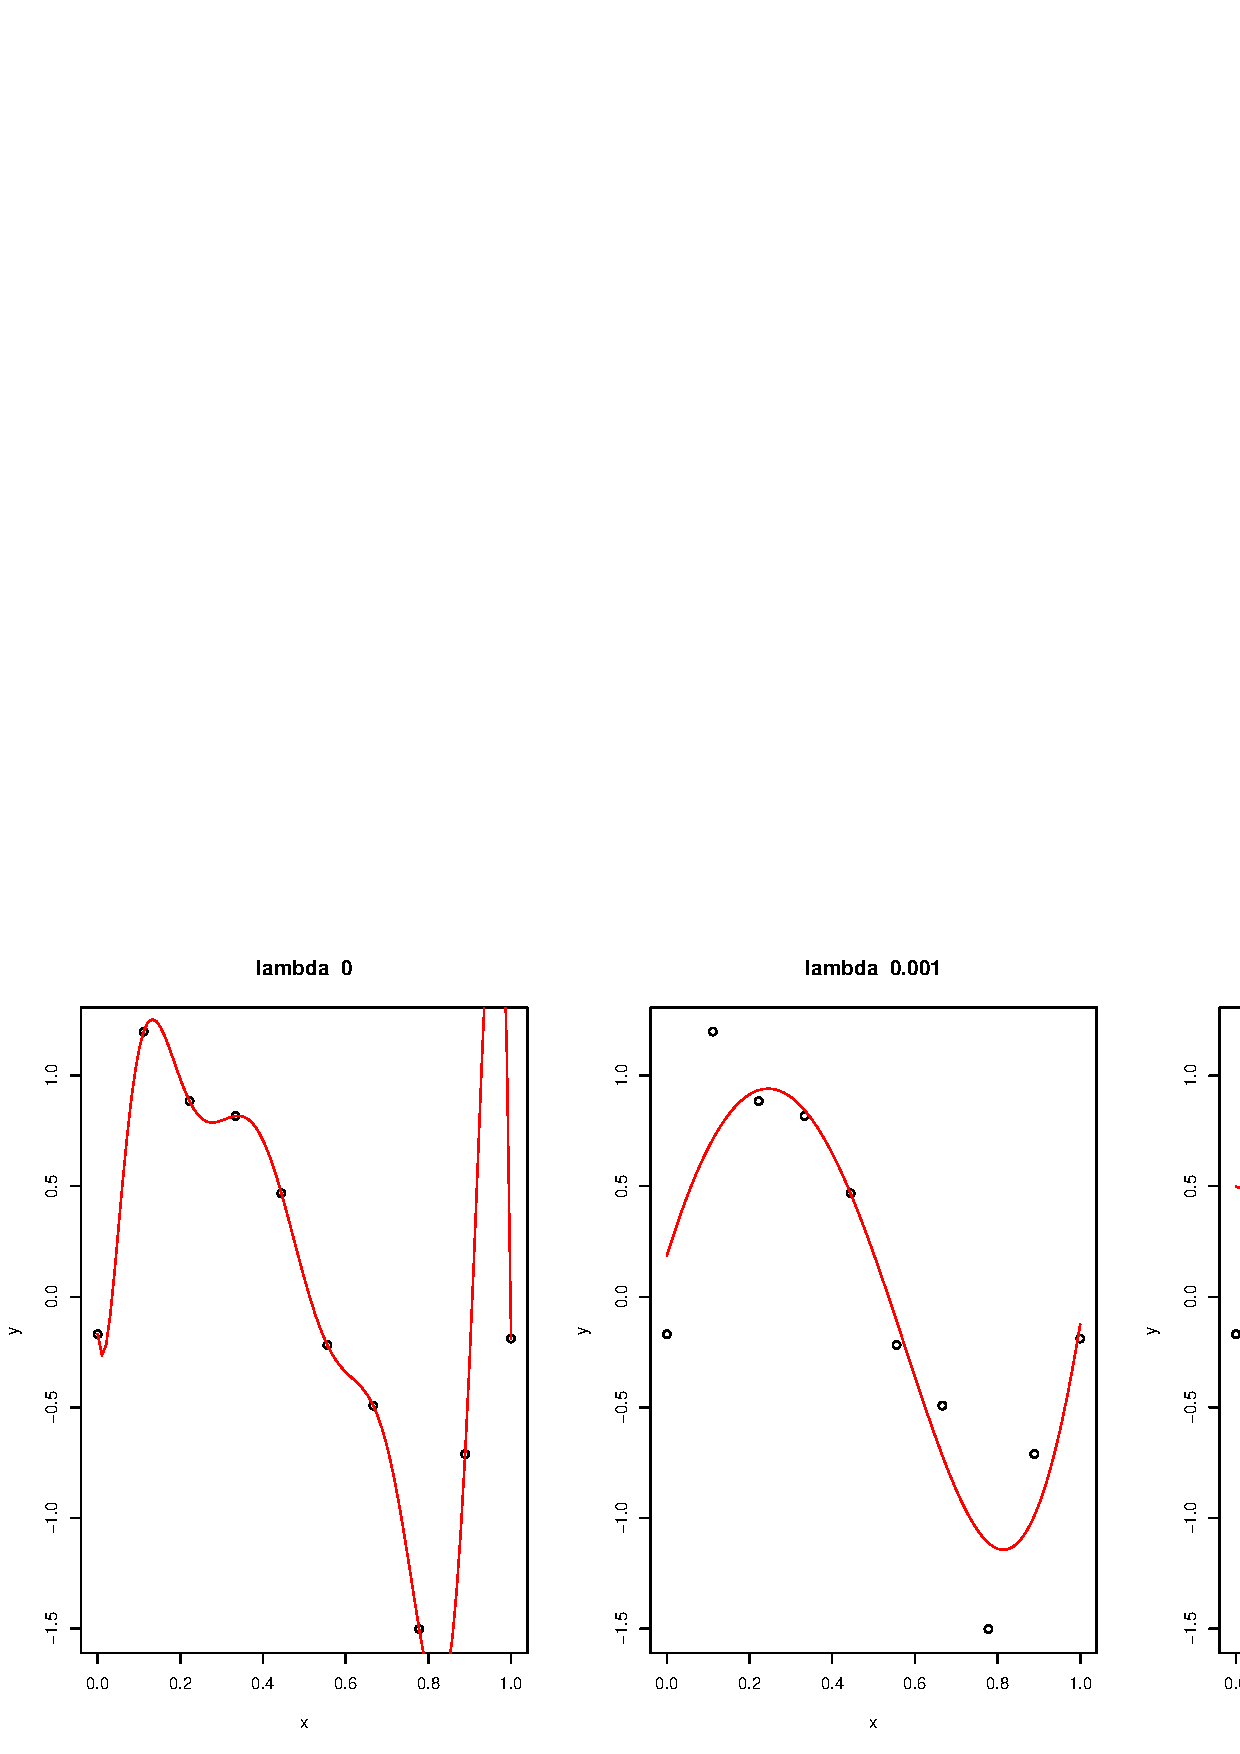
\includegraphics[width=\textwidth]{03Ann/regulariz/bgPolyM9regLambdas.png}
	\end{center}
	\caption[พหุนามระดับขั้นเก้า กับการทำค่าน้ำหนักเสื่อม]{พหุนามระดับขั้นเก้า กับการทำค่าน้ำหนักเสื่อม ด้วยลากรานจ์ค่าต่าง ๆ.
		ภาพซ้าย แสดงการโอเวอร์ฟิต ($\lambda = 0$).
		ภาพกลาง แสดงแบบจำลองที่เหมาะสม ($\lambda = 0.001$).
		ภาพขวา แสดงการอันเดอร์ฟิต ($\lambda = 1$).
	จุดวงกลม คือจุดข้อมูลฝึก และเส้นทึบสีแดง แสดงค่าที่แบบจำลองทำนาย.}
	\label{fig: bg poly M9 reg different lambdas}
\end{figure}
%

%
\begin{figure}
	\begin{center}
		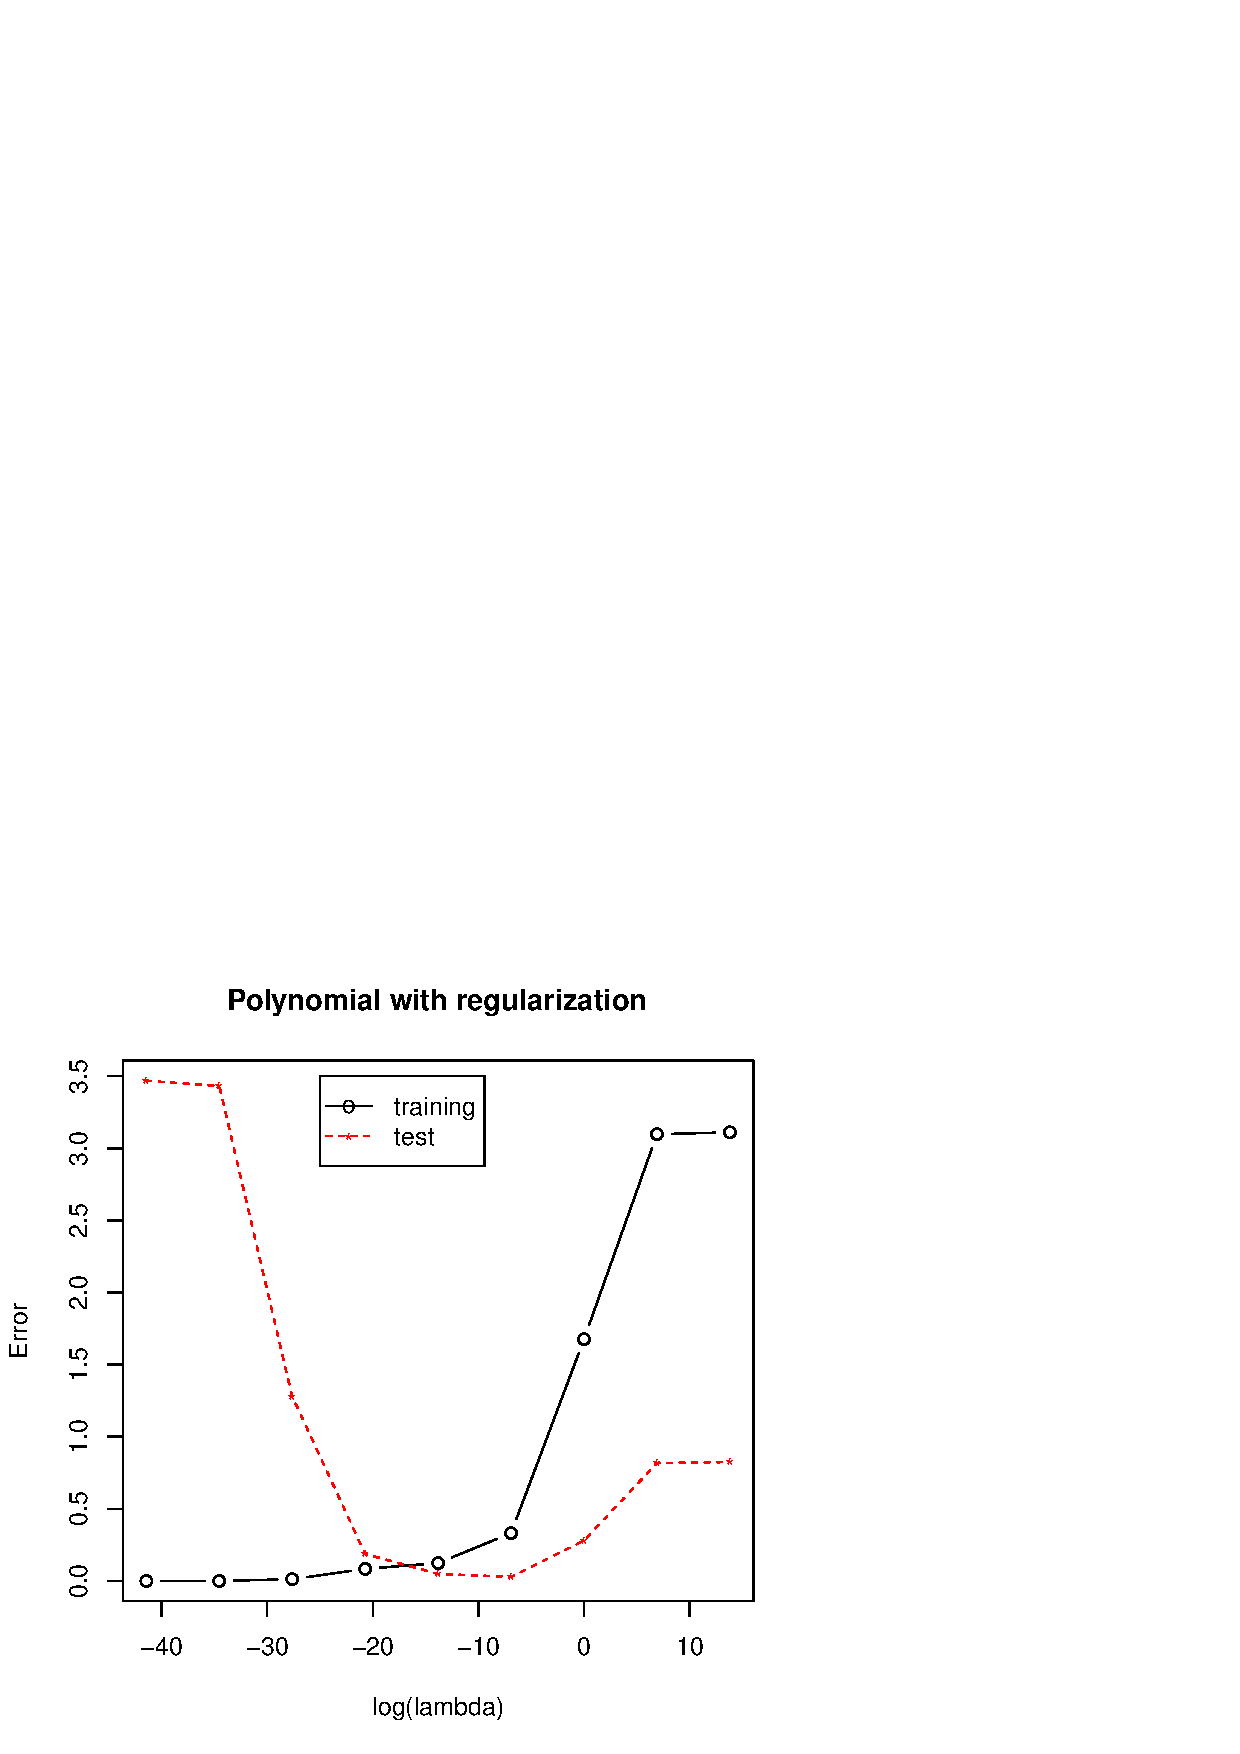
\includegraphics[height=4in]{03Ann/regulariz/bgPolyM9regTrainTest.png}
	\end{center}
	\caption[การทำน้ำหนักเสื่อมด้วยลากรานจ์ค่าต่าง ๆ]{การทำน้ำหนักเสื่อมด้วยลากรานจ์ค่าต่าง ๆ ประเมินด้วยข้อมูลชุดฝึกหัด (เส้นทึกสีดำ) กับ ชุดทดสอบ (เส้นประสีแดง). แกนตั้ง แสดงค่าผิดพลาด. แกนนอน แสดงค่าของ $\log \lambda$.}
	\label{fig: bg poly regularization evaluation}
\end{figure}
%

สำหรับการประเมินแบบจำลอง ปัจจัยสำคัญ คือ แบบจำลองสามารถทำนายข้อมูลที่ไม่เคยเห็นมาก่อนได้ดี 
หรือ แบบจำลองมี\textit{คุณสมบัติความทั่วไป}.
ดังนั้น 
เพื่อเลือกความซับซ้อนของแบบจำลอง เช่น การเลือกระดับขั้นของพหุนาม 
หรือการเลือกค่าลากรานจ์ของการทำค่าน้ำหนักเสื่อม 
จึงควรทำการวัด\textit{คุณสมบัติความทั่วไป}ของแบบจำลองที่ความซับซ้อนต่าง ๆ กัน.
วิธีที่ง่ายและตรงไปตรงมาที่สุด ก็คือ การแบ่งข้อมูลออกเป็น $2$ ชุด
ได้แก่ \textit{ข้อมูลชุดฝึก} ที่ใช้ฝึกแบบจำลอง นั่นคือใช้หาค่าของพารามิเตอร์ $\mathbf{w}$ 
และ\textit{ชุดตรวจสอบ}
% (validation set หรือ hold-out set) 
\index{english}{validation} 
\index{thai}{ข้อมูลชุดตรวจสอบ} 
ที่ใช้เลือกความซับซ้อนของแบบจำลอง เช่น $M$ หรือ $\lambda$.

หลังจากเลือกแบบจำลองเสร็จแล้ว 
เพื่อประเมินแบบจำลอง ควรจะใช้\textit{ข้อมูลชุดทดสอบ} ซึ่งเป็นข้อมูลอีกชุด สำหรับการทดสอบ.
การที่ต้องใช้\textit{ชุดทดสอบ}ที่แยกออกมานี้ เพื่อกันปัญหา ที่อาจจะเลือกแบบจำลองที่เกิดการโอเวอร์ฟิตกับชุดตรวจสอบได้.
หากทำการเลือกแบบจำลองได้ดี ค่าผิดพลาดที่ประเมินกับ\textit{ข้อมูลชุดทดสอบ} ไม่ควรห่างมากจากค่าผิดพลาดที่ประเมินกับ\textit{ข้อมูลชุดตรวจสอบ}.

\paragraph{ครอสวาลิเดชั่น.}
ถ้าข้อมูลมีจำนวนมาก
การแบ่งบางส่วนของข้อมูลมาเป็นชุดตรวจสอบนั้น ไม่ได้ดูว่ามีปัญหาอะไร
แต่หากข้อมูลมีปริมาณจำกัด ควรจะจัดการสถานการณ์อย่างไร 
เมื่อการฝึกแบบจำลองให้ดีต้องการข้อมูลจำนวนมาก
แต่คุณภาพของการตรวจสอบเลือกความซับซ้อน และการทดสอบ ก็ต้องการข้อมูลจำนวนมากเช่นกัน.
การแบ่งส่วนข้อมูลที่มีปริมาณน้อยอยู่แล้ว ยิ่งจะทำให้แต่ละส่วนมีปริมาณน้อยลงไปอีก.
วิธีหนึ่งที่ออกแบบมาเพื่อบรรเทาปัญหานี้ คือ การทำ\textit{ครอสวาลิเดชั่น} (cross-validation). \index{english}{cross-validation} 
\index{thai}{ครอสวาลิเดชั่น}
แนวคิดคือ การสุ่มและใช้ผลเฉลี่ย
โดยทำการฝึกแบบจำลองและการตรวจสอบหลาย ๆ ครั้ง 
แต่ละครั้ง แบ่งข้อมูลต่าง ๆ กันไป
แล้วเอานำผลลัพธ์ที่ได้มาเฉลี่ยกัน เพื่อสรุปหาแบบจำลองที่มี\textit{คุณสมบัติความทั่วไป}ดีที่สุด.
การดำเนินการ จะแบ่งข้อมูลออกเป็น $K$ ส่วน 
แต่ละครั้งจะเลือกส่วนหนึ่งมาเป็น\textit{ชุดตรวจสอบ}
และใช้ส่วนที่เหลือ ($K-1$ ส่วน) สำหรับฝึกแบบจำลอง.
เนื่องจาก การแบ่งข้อมูลเป็น $K$ ส่วน 
วิธีนี้ มักถูกเรียกว่า วิธีครอสวาลิเดชั่น $K$ พับ (K-fold cross-validation).

วิธีครอสวาลิเดชั่น $K$ พับทำการฝึกและตรวจสอบ $K$ ครั้ง
ที่แต่ละครั้งจะเลือกส่วนที่ทำการตรวจสอบแตกต่างกัน.
เมื่อทำจนครบทุกส่วนแล้ว จึงนำผลประเมินจากแต่ละครั้ง รวม $K$ ค่า มาหาค่าเฉลี่ย เป็น\textit{ค่าประเมินครอสวาลิเดชั่น}ของแบบจำลอง (cross-validation evaluation).
\textit{ค่าประเมินครอสวาลิเดชั่น}นี้
สามารถใช้เปรียบเทียบกับแบบจำลองอื่น (หรือแบบจำลองเดียวกันแต่ความซับซ้อนอื่น) เพื่อหาแบบจำลอง(หรือความซับซ้อน)ที่ดีที่สุด.

%
\begin{figure}
	\begin{center}
		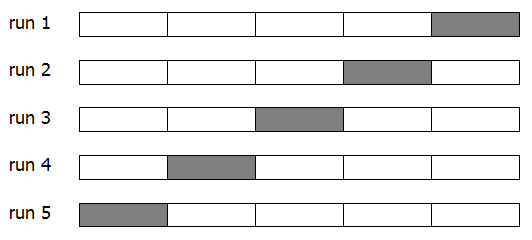
\includegraphics[height=2in]{03Ann/regulariz/crossvalidation.png}
	\end{center}
	\caption[วิธีครอสวาลิเดชั่นห้าพับ]{วิธีครอสวาลิเดชั่น $5$ พับ. 
		ข้อมูลทั้งหมดจะถูกแบ่งออกเป็น $5$ ส่วน 
		และวิธีครอสวาลิเดชั่นจะทำทั้งหมด $5$ ครั้ง
		โดยแผนภาพแสดงในเห็นว่า การทำครั้งแรกใช้ข้อมูล $4$ ส่วนแรกสำหรับการฝึก และส่วนสุดท้ายสำหรับการตรวจสอบ.
		ส่วนที่ใช้สำหรับการตรวจสอบ แสดงเป็นสีเข้ม.
		ครั้งที่สอง สาม สี่ และห้าก็ทำเช่นเดิม เพียงแต่เปลี่ยนส่วนที่ทำการตรวจสอบ.
	}
	\label{fig: bg cross validation}
\end{figure}
%

รูป~\ref{fig: bg cross validation} แสดงแผนภาพการแบ่งข้อมูลสำหรับวิธีครอสวาลิเดชั่น $5$ พับ ($K=5$) และการจัดสรรข้อมูลสำหรับการฝึก และการตรวจสอบในแต่ละครั้ง. 
การฝึกและตรวจสอบแต่ละครั้ง
จะเรียกเป็น\textit{วาลิเดชั่นรัน} (validation run).
ในภาพแสดง $5$ \textit{วาลิเดชั่นรัน} 
ที่รันแรก (Run 1) ฝึกแบบจำลองด้วยข้อมูล $4$ ส่วนแรก 
และนำแบบจำลองที่ฝึกแล้ว ไปตรวจสอบกับข้อมูลส่วนหลังสุด (แรงเงาสีเข้มในรูป).
รันที่สอง ฝึกแบบจำลองด้วยข้อมูลส่วนอื่นยกเว้นส่วนที่ $4$ (แรงเงา) 
แล้วตรวจสอบกับส่วนที่ $4$ ที่กันออกไว้.
ทำเช่นนี้จนครบ $5$ รัน แล้วนำเอาผลที่ได้มาเฉลี่ย.

ด้วยวิธีนี้ แต่ละรันจะฝึกแบบจำลองด้วยข้อมูลขนาด $K-1$ ส่วนของที่มีอยู่ทั้งหมด $K$ ส่วน 
และผลค่าผิดพลาดจากการตรวจสอบ เป็นค่าเฉลี่ยของค่าผิดพลาดที่ได้จากทุกส่วนของข้อมูล.
วิธีครอสวาลิเดชั่นนี้ ทำให้เสมือนว่ามีข้อมูลมากขึ้น ทั้งการฝึกและการตรวจสอบ.
%ซึ่งเมื่อได้ผลเปรียบเทียบจากครอสวาลิเดชั่นแล้ว เราก็จะสามารถเลือกแบบจำลองได้จาก.

แม้วิธีครอสวาลิเดชั่น
จะบรรเทาปัญหาของขนาดข้อมูลที่จำกัด และเป็นวิธีที่ใช้ข้อมูลได้อย่างคุ้มค่า
แต่ข้อเสียของวิธีครอสวาลิเดชั่นคือ การที่ต้องทำการรันทั้งหมด $K$ ครั้ง.
ถ้าเลือกค่า $K$ ใหญ่ ก็จะเปรียบเสมือนได้ใช้ข้อมูลปริมาณมากในการฝึก
แต่ข้อเสีย คือเท่ากับเพิ่มจำนวนรันด้วย
โดยเฉพาะ ถ้าการรันแต่ละครั้งใช้เวลามาก.
กล่าวอีกนัยก็คือ วิธีครอสวาลิเดชั่น
ใช้การคำนวณที่เพิ่มขึ้น เพื่อบรรเทาปัญหาข้อมูลปริมาณน้อย.
ดังนั้น หากถ้าการรันแต่ละครั้งใช้การคำนวณมากอยู่แล้ว แนวทางของวิธีครอสวาลิเดชั่นอาจจะไม่เหมาะสม.
%เช่น การฝึกแบบจำลองอาจจะมีการคำนวณสูง
%หรือการทำครอสวาลิเดชั่นกับแบบจำลองที่มีพารามิเตอร์ที่ควบคุมความซับซ้อนหลายตัว
%อาทิ การทำเรกูลาไรเซชั่นด้วยลากรานจ์พารามิเตอร์หลายตัว อาจทำปริมาณการคำนวณเพิ่มขึ้นมหาศาล.


%LATER
%\section{คำสาปของมิติ}
%\label{sec: curses of dimensionality}

{\small
	\begin{shaded}
\paragraph{\small เกร็ดความรู้เซลล์ประสาท}
(เรียบเรียงจาก \cite{BuddhasBrain} และ \cite{Wikipedia})
		\index{thai}{เซลล์ประสาท}
		\index{english}{Biological Neurons}
		\index{english}{side story}
		\index{english}{side story!Neurons}
		\index{thai}{เกร็ดความรู้}
		\index{thai}{เกร็ด!เซลล์ประสาท}
		
%\footnote{จาก \url{https://en.wikipedia.org/wiki/Brain_size} (สืบค้น 21 ส.ค. 2559)}
สมองมนุษย์ประกอบด้วยเซลล์ชนิดต่าง ๆ มากมาย
		เช่น 
		เส้นเลือด 
		เซลล์เกลีย
		เซลล์ประสาท.
		เส้นเลือดทำหน้าที่รับส่งอากาศ น้ำ อาหาร.
		\textit{เซลล์เกลีย}(neuroglia) ทำหน้าที่สนับสนุนต่าง ๆ รวมถึงการรักษา\textit{ภาวะธำรงดุล} (homeostasis) เพื่อให้ภายในสมองมีสภาวะที่เหมาะ เช่น การควบคุมระดับความเข้มข้นของโซเดียมและแคลเซียมไอออน.
		%ซึ่งในจำนวนนั้น 
		เซลล์ประสาททำหน้าที่หลักของสมอง ได้แก่การควบคุมระบบการทำงานต่าง ๆ ในร่างกายให้เป็นปกติ 
		รวมไปถึง การให้ความสามารถในการจำ การเรียนรู้ การคิด การรับรู้ และการตอบสนอง.
		
		สมองมนุษย์มีเซลล์ประสาทอยู่ประมาณแสนล้านเซลล์ 
		เซลล์ประสาทเองก็มีอยู่หลายประเภท แต่โครงสร้างพื้นฐานมีลักษณะคล้าย ๆ กัน.
		%
		นั่นคือ
		เซลล์ประสาทแต่ละเซลล์
		มีใยประสาทเพื่อรับสัญญาณเข้าสู่เซลล์
		เรียกว่า \textit{เดนไดรต์} (dendrite).
		สัญญาณต่าง ๆ 
		ทั้งสัญญาณกระตุ้นและสัญญาณยับยั้งที่เข้าสู่เซลล์
		จะถูกนำมารวมกันที่นิวเคลียส
		และผลรวมของสัญญาณที่รับเข้ามา  
		จะเป็นตัวตัดสินว่า
		เซลล์ประสาทนั้นจะอยู่ในสถานะถูกกระตุ้นหรือไม่.
		ถ้าเซลล์ประสาทอยู่ในสถานะถูกกระตุ้น มันจะส่งสัญญาณออกไปให้กับเซลล์ประสาทอื่น ๆ ที่รับสัญญาณจากมัน
		โดยส่งออกผ่านใยประสาทนำออกสัญญาณ
		เรียกว่า \textit{แอกซอน} (axon). 
		จุดต่อระหว่างแอกซอนของเซลล์ประสาทตัวหนึ่งกับเดนไดรต์ของเซลล์ประสาทอีกเซลล์หนึ่ง 
		%เซลล์ประสาทแต่ละเซลล์เชื่อมต่อกับเซลล์ประสาทอื่น ๆ ผ่าน
		เป็นจุดประสานประสาทที่เรียกว่า \textit{ไซแนปส์} (synapse).
		แนวคิดพื้นฐานนี้เองที่ \textit{โรเซนแบลท} (หัวข้อ~\ref{sec: ann}) นำไปสร้างแบบจำลอง\textit{เพอร์เซปตรอน} (ดูรูป~\ref{fig: ANN neuron} และ \ref{fig: ANN synapse} ประกอบ)
		เมื่อเปรียบเทียบเพอร์เซปตรอน (รูป~\ref{fig: ANN perceptron})
		กับเซลล์ประสาท ผลคูณของอินพุตกับค่าน้ำหนักของเพอร์เซปตรอน (เช่น $x_1 w_1$ และ $x_2 w_2$) เทียบได้กับ ความแรงของสัญญาณประสาท แต่ละสัญญาณที่รับเข้ามาผ่านไซแนปส์
		แล้วเดินทางเข้าสู่นิวเคลียสของเซลล์ประสาท
		เพื่อไปรวมกับความแรงของสัญญาณประสาทที่รับเข้ามาผ่านไซแนปส์จุดอื่น ๆ.
		ความแรงของสัญญาณประสาท แต่ละสัญญาณที่รับเข้ามาผ่านไซแนปส์ จะขึ้นอยู่กับ
		สัญญาณที่ส่งมา (เปรียบเทียบกับ $x_i$) และ ความแข็งแรงในการเชื่อมต่อสัญญาณของไซแนปส์ (เปรียบเทียบกับ $w_i$).
		
		โดยเฉลี่ยแล้ว เซลล์ประสาทแต่ละเซลล์จะมีไซแนปส์ประมาณห้าพันจุด
		ซึ่งนั่นคือเมื่อรวมแล้ว ในสมองมนุษย์หนึ่งคนจะมีการเชื่อมต่อประสาทอยู่ราว ๆ ห้าร้อยล้านล้านไซแนปส์.
		การรับส่งสัญญาณประสาทระหว่างเซลล์ประสาทมีหลายกลไก เช่น กลไกทางเคมี (ผ่านสารสื่อประสาท) กลไกทางไฟฟ้า และ กลไกเชิงภูมิคุ้มกัน.
		แต่กลไกหลักของการส่งสัญญาณประสาทคือกลไกทางเคมี
		ซึ่งคือการรับส่งสัญญาณประสาทระหว่างเซลล์ประสาทโดยดำเนินการผ่าน\textit{สารสื่อประสาท} (neurotransmitter). 
		เซลล์ประสาทที่ส่งสัญญาณจะปล่อยสารสื่อประสาทออกมา
		ผ่านโปรตีนที่ทำหน้าที่ส่งสารสื่อประสาท.
		โปรตีนส่งสาร เรียกว่า \textit{ทรานสปอร์ตเตอร์} (neurotransmitter transporter). 
		และเซลล์ประสาทที่รับสัญญาณ จะรับสารสื่อประสาทเหล่านั้น
		ด้วยโปรตีนที่ทำหน้าที่รับสารสื่อประสาท.
		โปรตีนรับสาร เรียกว่า \textit{รีเซปเตอร์} (receptor).
		% 220 MPH speed of neural impulse\cite{GodwinCham2012a}
		
		
		%[กลไกของ chemical synapse: binding to response]
		เมื่อรีเซปเตอร์ได้รับสารสื่อประสาท
		นั่นคือ โครงสร้างของสารสื่อประสาทจับกับโครงสร้างของรีเซปเตอร์
		แล้วทำให้กลไกของรีเซปเตอร์เปิดทำงาน
		%เพื่อรับโมเลกุลของสารสื่อประสาทเข้าสู่เซลล์ประสาท.
		%
		โมเลกุลที่จับกับรีเซปเตอร์ จะเรียกว่า \textit{ลิแกนต์} (ligand).
		กลไกของการจับตัวระหว่างรีเซปเตอร์กับลิแกนต์นี้
		จะเป็นกลไกในลักษณะ\textit{แม่กุญแจกับลูกกุญแจ} (lock and key).
		นั่นคือ โครงสร้างของรีเซปเตอร์แต่ละชนิดจะจับตัวได้เฉพาะกับลิแกนต์ที่มีโครงสร้างที่เข้ากันได้เท่านั้น
		เช่น สารสื่อประสาท\textit{อาเซ็ตทิลคอลีน} (acetylcholine) ซึ่งเป็นสารสื่อประสาทที่เซลล์ประสาทใช้ติดต่อกระตุ้นเซลล์กล้ามเนื้อ
		จะจับกับรีเซปเตอร์สำหรับอาเซ็ตทิลคอลีนได้เท่านั้น
		และ รีเซปเตอร์สำหรับสารสื่อประสาทตัวอื่น ก็ไม่อาจจับกับอาเซ็ตทิลคอลีนได้เช่นกัน.
		การเข้าใจกลไกการทำงานลักษณะนี้ 
		ช่วยให้เภสัชศาสตร์สามารถออกแบบตัวยาที่เฉพาะเจาะจงกับสารสื่อประสาทเฉพาะตัวได้
		เช่น ยาต้านอาการเศร้าซึม \textit{ฟลูโอเซตทีน} (Fluoxetine) ที่เฉพาะเจาะจงกับสารสื่อประสาท\textit{เซอโรโทนิน} (Serotonin).
		
		หมายเหตุ เซลล์ประสาทแต่ละชนิดจะมีลักษณะเฉพาะตัวต่างกันและจะทำงานกับสารสื่อประสาทเฉพาะชนิด
		เช่น
		\textit{เซลล์ประสาทเซอโรโทนิน} (serotonin neurons) ที่อยู่บริเวณ\textit{ดอร์ซอลราฟีนูเคลียส} (dorsal raphe nucleus) ของก้านสมอง จะทำงานกับสารสื่อประสาทเซอโรโทนิน\cite{LiEtAl2016a},
		\textit{เซลล์ประสาทซีเอ1พีรามิดอล} (CA1 pyramidal neurons) ที่อยู่บริเวณ\textit{ซีเอ1} (CA1) ของฮิปโปแคมปัส
		จะทำงานกับสารสื่อประสาท\textit{กลูตาเมท}(Glutamate)\cite{NeuroBank},
		\textit{เซลล์ประสาทมิดเบรนโดพามิเนอจิก} (midbrain dopaminergic neurons) ที่อยู่หลาย ๆ  บริเวณรวมถึง \textit{พื้นที่เวนทรอลเทกเมนทอล} (ventral tegmental area) ในสมองส่วนกลาง
		จะทำงานกับสารสื่อประสาท\textit{โดพามีน} (Dopamine)\cite{NeuroBank}.
		เซลล์ประสาทบางชนิดทำงานกับสารสื่อประสาทมากกว่าหนึ่งชนิด เช่น
		เซลล์ประสาทหนามกลาง (medium spiny neurons) ที่อยู่บริเวณบาซอลแกงเกลีย
		ส่งสัญญาณออกผ่าน\textit{กาบา} (GABA) แต่สามารถรับสัญญาณผ่านสารสื่อประสาทหลายชนิดรวมถึงกลูตาเมทและโดพามีน.
		
		%$\Box$
	\end{shaded}
}

%
\begin{figure}
	\begin{center}
		\begin{tabular}{cc}
			\includegraphics[height=1.8in]{03Ann/ann/Synapse1.png}
			&
			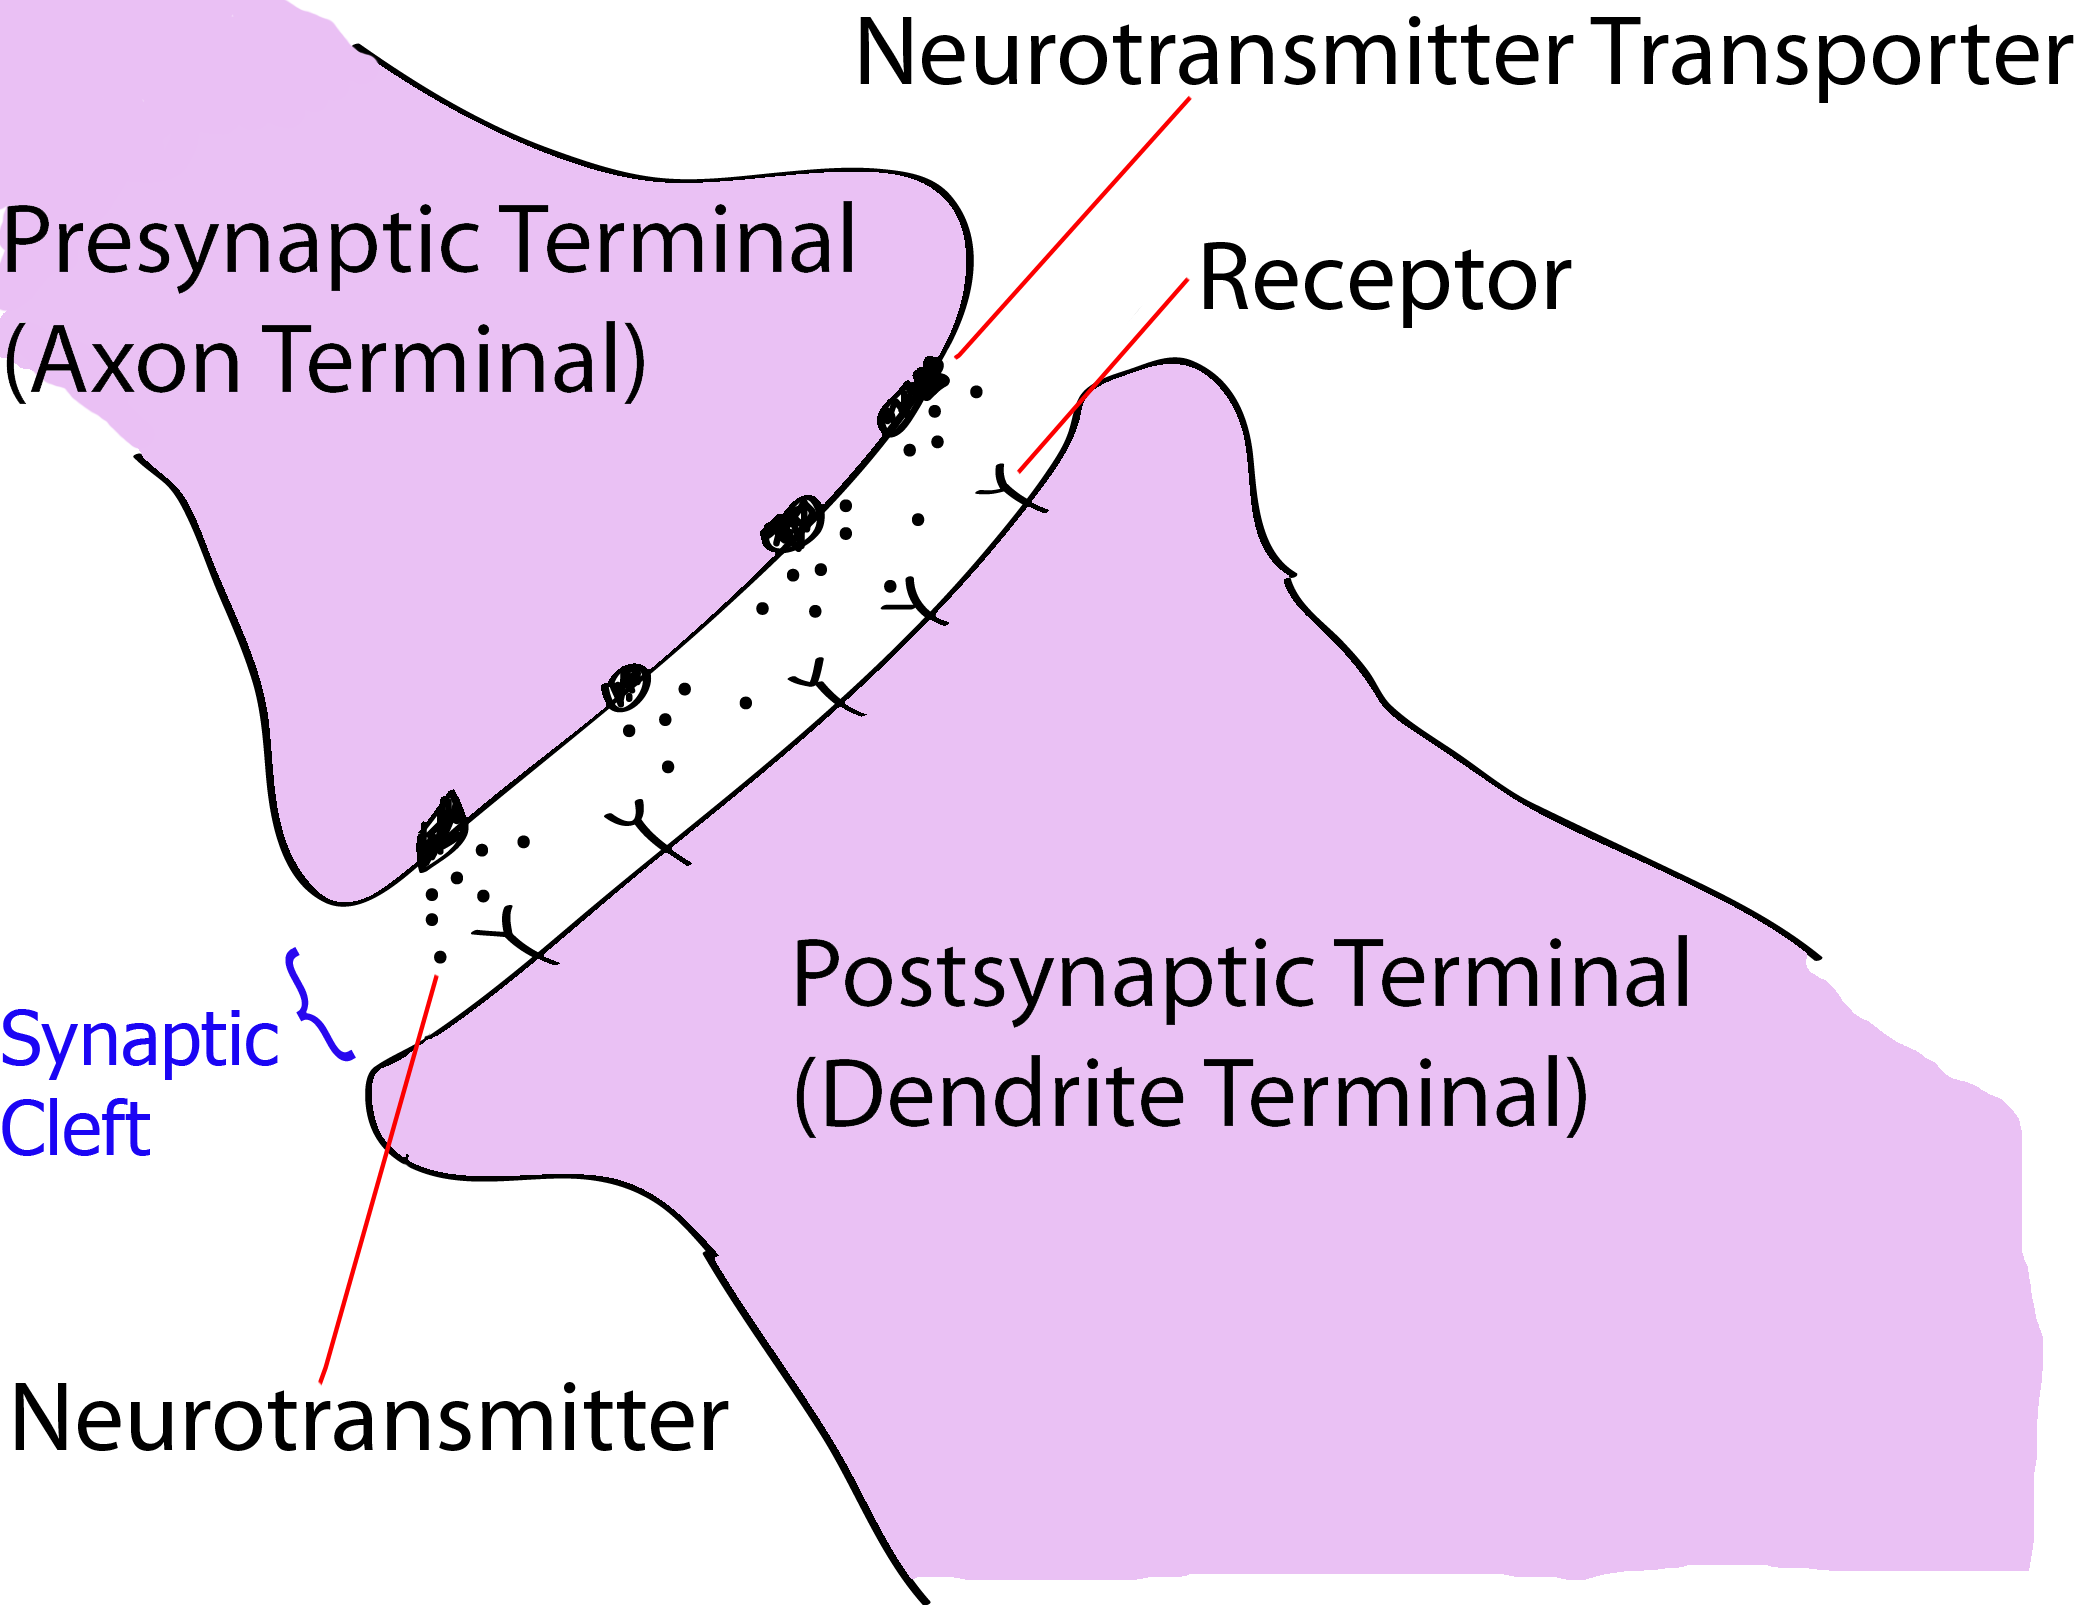
\includegraphics[height=1.8in]{03Ann/ann/chemicalSynapseCol.png}
			\\
			(ก) & (ข) \\
		\end{tabular} 
		
	\end{center}
	\caption[ไซแนปซ์]{ภาพแสดงเซลล์ประสาทเชื่อมต่อสัญญาณกันผ่าน\textit{ไซแนปซ์} 
		โดยสัญญาณที่สื่อสารกันนั้นทำโดยผ่านกลไกของ\textit{สารสื่อประสาท}.
		ภาพ ก แสดงเซลล์ทางซ้ายมือส่งสัญญาณผ่านไซแนปซ์ ไปสู่เซลล์ทางขวามือ.
%		{\footnotesize 
%			(ภาพดัดแปลงจาก \texttt{http://en.wikipedia.org/wiki/File:Neuron\_Hand-tuned.svg})
%		}
		ภาพ ข แสดงภาพขยายส่วนของไซแนปส์ ซึ่ง\textit{ส่วนปลายของแอกซอน} (presynaptic terminal) จะส่งสารสื่อประสาทออกมา และ\textit{ส่วนปลายของเดนไดรต์} (postsynaptic terminal) จะรับสารสื่อประสาท.
	}
	\label{fig: ANN synapse}
\end{figure}
%


\section{โครงข่ายประสาทเทียม}
\label{sec: ann}


%LATER
%\begin{minipage}{5.5in}
%{\small
%	\begin{shaded}
%		\paragraph{\small เกร็ดความรู้ เรื่องราวของการสอนเครื่องให้เรียน}
%		\index{side story}
%		\index{side story!ANN history}
%		\index{เกร็ดความรู้}
%		\index{เกร็ด!เรื่องของโครงข่ายประสาทเทียม}
%		
%		ประวัติย่อของ ANN.
%		... จาก Rosenblatt ... AI winter ... Backpropagation ... SVM ... Deep learning
%		+ Deep learning
%		
%		\cite{GoodfellowEtAl2016} Historial Trends in Deep Learning (\textsection 1.2)
%		
%		
%		% start two column, bilingual environment
%		\begin{Parallel}[c]{0.54\textwidth}{0.41\textwidth}
%			\selectlanguage{english}
%			\ParallelLText{
%				``dummy.''
%				\\
%				---Sean B. Carroll
%			}
%			\selectlanguage{thai}
%			\ParallelRText{
%				``dummy.'' \\
%				----ฉอน บี คาโรล
%			}
%		\end{Parallel}
%		\index{quote}
%		\index{quote!regulation}
%		
%		
%		
%	\end{shaded}
%}
%\end{minipage}

\textbf{โครงข่ายประสาทเทียม} (Artificial Neural Network)
\index{thai}{โครงข่ายประสาทเทียม}
\index{english}{Artificial Neural Network คำย่อ ANN}
เป็นแบบจำลองทำนาย
ที่ใช้ลักษณะการคำนวณง่าย ๆ คล้าย ๆ กัน จำนวนมาก
ที่เมื่อนำมารวมกันแล้ว ให้ผลโดยรวม เป็นแบบจำลองทำนายที่มีความสามารถสูง.
%โดยในยุคเริ่มแรก
%\textit{โครงข่ายประสาทเทียม}
%ได้รับแรงบันดาลใจ จากโครงข่ายประสาททางชีววิทยา (biological neural networks).

\textit{โครงข่ายประสาทเทียม} มีอยู่หลายชนิด
หนึ่งในชนิดที่สำคัญและได้รับความนิยมอย่างมาก
คือ \textit{เพอร์เซปตรอนหลายชั้น}.
\textbf{เพอร์เซปตรอนหลายชั้น} (multi-layer perceptron คำย่อ MLP)
\index{english}{multi-layer perceptron}
\index{english}{MLP}
\index{thai}{เพอร์เซปตรอนหลายชั้น}
ที่รวมการคำนวณของหน่วยคำนวณย่อย ที่เรียกว่า 
\textit{เพอร์เซปตรอน} หลาย ๆ หน่วย
เข้าด้วยกัน
ในลักษณะเป็นชั้น ๆ.

หน่วยคำนวณย่อย \textbf{เพอร์เซปตรอน} (perceptron)
\index{thai}{เพอร์เซปตรอน}
\index{english}{perceptron}
ถูกพัฒนาโดยการเลียนแบบเซลล์ประสาทของสิ่งมีชีวิต.
%
เซลล์ประสาทของสิ่งมีชีวิตมีอยู่หลายชนิด
แต่มีลักษณะทั่ว ๆ ไป 
ดังแสดงในรูป~\ref{fig: ANN neuron}.
แต่ละเซลล์รับสัญญาณกระตุ้นจากเซลล์อื่น ๆ ผ่าน\textit{เดนไดรต์} (dendrite)
เมื่อผลรวมของสัญญาณกระตุ้นมากพอเซลล์จะเข้าสู่สถานะถูกกระตุ้น และส่งสัญญาณออกผ่าน\textit{แอกซอน} (axon)
ไปให้เซลล์อื่น ๆ ต่อไป.
ความแรงของสัญญาณกระตุ้นที่รับมาจากแต่ละเซลล์ก็ต่าง ๆ กันไป ขึ้นกับการเชื่อมต่อ ซึ่งความแข็งแรงของการเชื่อมต่อ ก็มีการปรับเปลี่ยนตามการใช้งาน.

%
\begin{figure}
	\begin{center}
		\includegraphics[height=3in]{03ANN/ann/typicalNeuron1.png}
	\end{center}
	\caption[เซลล์ประสาท]{รูปแสดงโครงสร้างของเซลล์ประสาททั่ว ๆ ไป
		\textit{เดนไดรต์}  ทำหน้าที่เสมือนอินพุตของเซลล์ 
		และ \textit{แอกซอน}  ทำหน้าที่เสมือนกับเอาต์พุตของเซลล์. 
เมื่อสัญญาณกระตุ้นจากอินพุตรวมกันมากพอ
เซลล์จะเข้าสู่สถานะถูกกระตุ้น 
และส่งการกระตุ้นออกต่อไป ผ่าน\textit{แอกซอน}.
%		{\footnotesize 
%			(ภาพวาดขึ้น โดยดัดแปลงจาก \texttt{http://en.wikipedia.org/wiki/File:Neuron\_Hand-tuned.svg})
%		}
	}
	%:////en.wikipedia.org//wiki//File:Neuron_Hand-tuned.svg}.}
	\label{fig: ANN neuron}
\end{figure}
%

แฟรงค์ โรเซนแบลท (Frank Rosenblatt) ออกแบบ สร้าง และได้สาธิตการทำงานของ
เพอร์เซปตรอน 
ที่สร้างด้วยวงจรไฟฟ้า
เพื่อจำลองการทำงานของเซลล์ประสาท
ในปี 1957. 
รูป~\ref{fig: ANN perceptron} แสดงโครงสร้างแนวคิดของเพอร์เซปตรอน.

%
\begin{figure}
	\begin{center}
		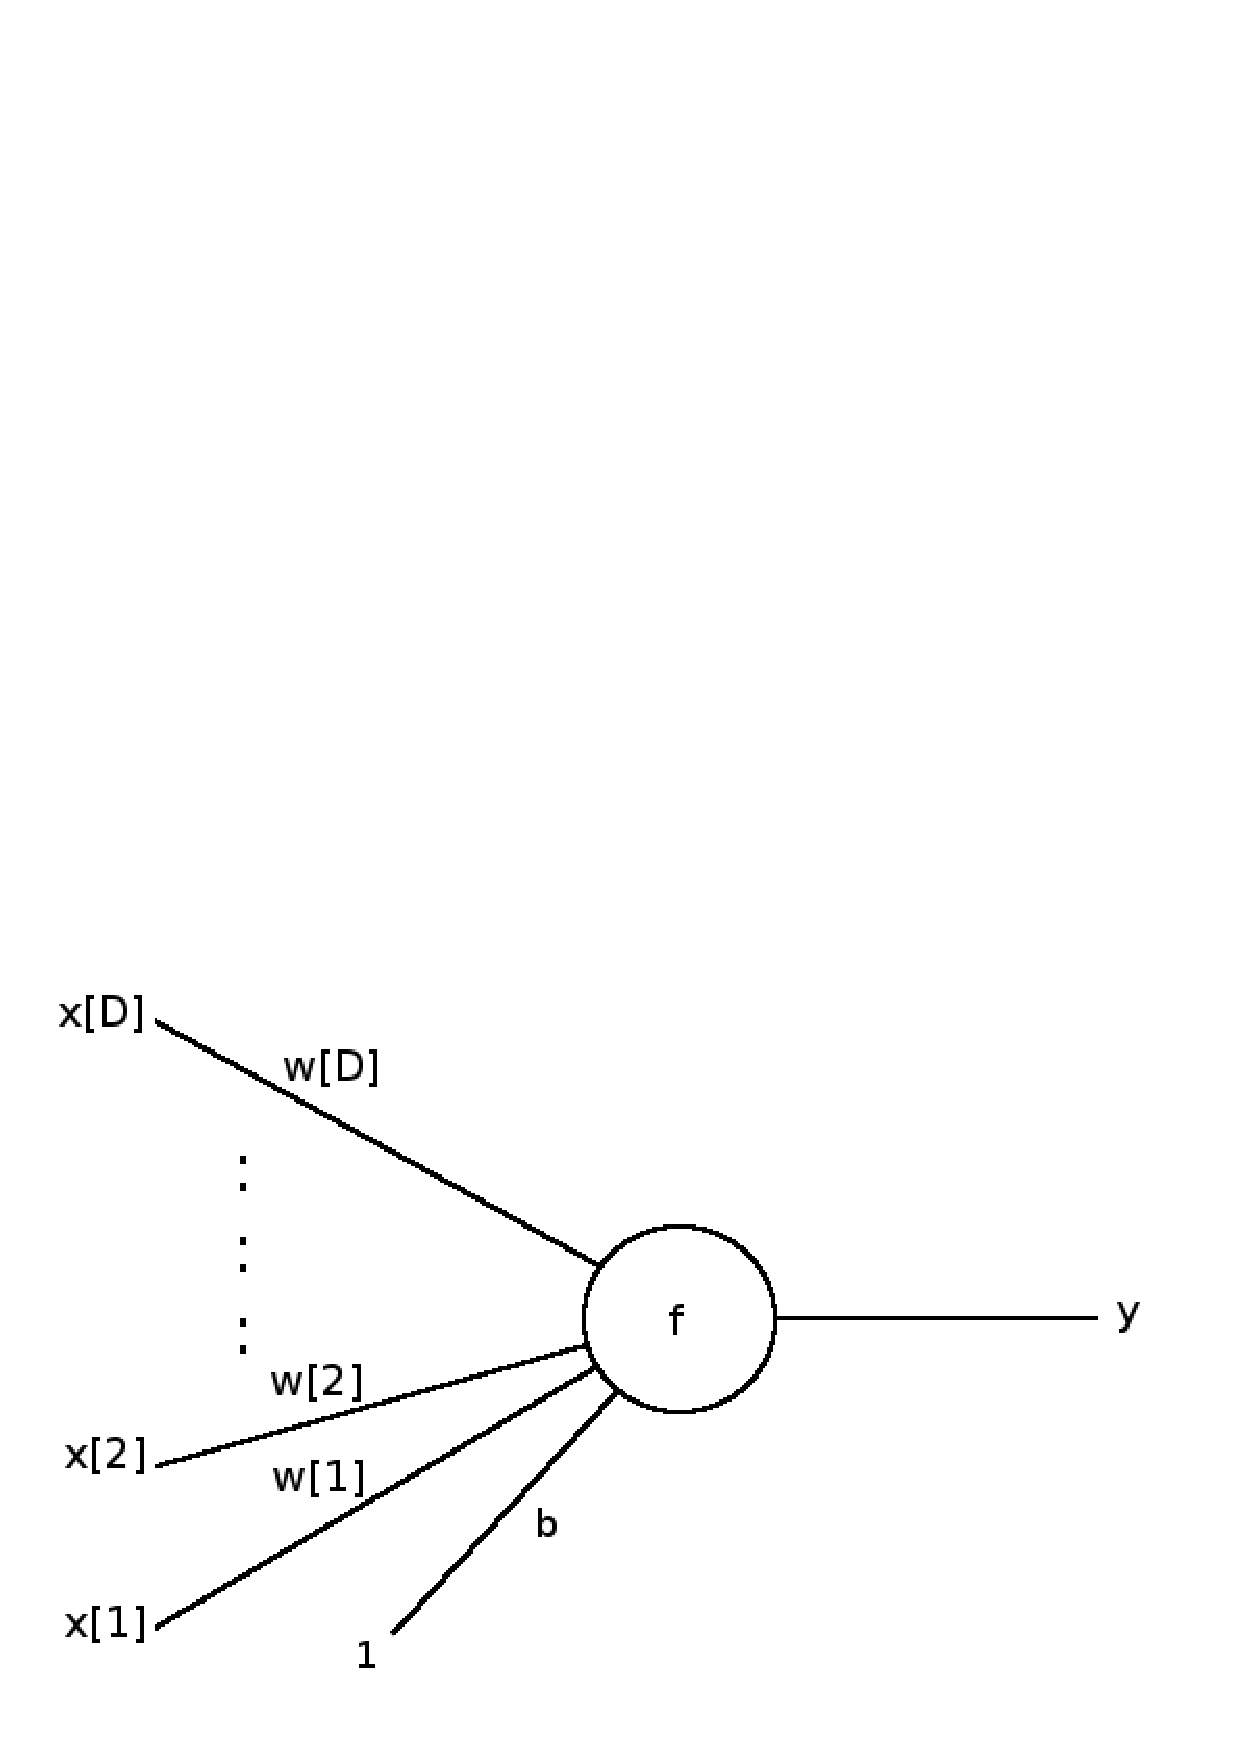
\includegraphics[height=3in]{03ANN/ann/perceptron.png}
	\end{center}
	\caption[เพอร์เซปตรอน]{แผนผังแสดงโครงสร้างของเพอร์เซปตรอน ที่เอาต์พุต $y$ แสดงสถานะของหน่วยประสาทเทียม
	โดย หน่วยประสาทเทียมจะอยู่ในสถานะถูกกระตุ้น เมื่อผลรวมสัญญาณกระตุ้น ซึ่งคือ $w_1 \cdot x_1 + w_2 \cdot x_2 + \ldots + w_D \cdot x_D$ มีค่ามากพอ (มากถึงหรือเกินค่าระดับกระตุ้น $\tau$).
	ค่า $x_1, \ldots, x_D$ เป็นอินพุตต่าง ๆ ของเพอร์เซปตรอน.
	ค่า $w_1, \ldots, w_D$ เป็นค่าน้ำหนัก แสดงความแข็งแรงของการเชื่อมต่อกับแต่ละอินพุต.
%	  $y = h(b + w_1 \cdot x_1 + w_2 \cdot x_2 + \ldots + w_D \cdot x_D)$ เมื่อ ฟังก์ชันกระตุ้น $f$ เป็น\textit{ฟังก์ชันจำกัดแข็ง}.
  }
	\label{fig: ANN perceptron}
\end{figure}
%

การคำนวณของเพอร์เซปตรอน
ดำเนินการ โดย การนำอินพุตแต่ละตัว
ไปคูณกับค่าน้ำหนักของอินพุตนั้น ๆ 
และนำค่าผลคูณทั้งหมดมาบวกกัน.
แล้วหากผลบวกมีค่ามากพอ 
นั่นคือ มีค่าเท่ากับหรือมากกว่า\textit{ค่าระดับกระตุ้น}  เพอร์เซปตรอนจะอยู่ในสถานะถูกกระตุ้น (ให้เอาต์พุตเป็น $1$)
แต่หากผลบวกมีค่าน้อยกว่าระดับกระตุ้น 
เพอร์เซปตรอนจะอยู่ในสถานะไม่ถูกกระตุ้น (ให้เอาต์พุตเป็น $0$).
ดังนั้น เอาต์พุตของเพอร์เซปตรอน สามารถเขียนดังสมการ~\ref{eq: perceptron neural sim}.
\begin{eqnarray}
y = \left\{
\begin{array}{l l}
0 & \quad \mbox{เมื่อ} \quad w_1 x_1 + \cdots + w_D x_D < \tau , \\
1 & \quad \mbox{เมื่อ} \quad w_1 x_1 + \cdots + w_D x_D \geq \tau .
\end{array} \right.
\label{eq: perceptron neural sim}
\end{eqnarray}
เมื่อ $w_1, \ldots, w_D$ เป็น\textbf{ค่าน้ำหนัก} (weights)
\index{thai}{ค่าน้ำหนัก}
\index{english}{weights}
ของอินพุต $x_1, \ldots, x_D$ ตามลำดับ
และ
$\tau$ คือ ค่าระดับกระตุ้น
โดยผลลัพธ์ $y = 1$ 
แทนสถานะการถูกกระตุ้น 
และ $y = 0$ แทนสถานะไม่ถูกกระตุ้น.
%
บางครั้ง อินพุต $x_1, \ldots, x_D$
อาจถูกมองรวม คือมองเป็น
อินพุต $\bm{x} = [x_1, \ldots, x_D]^T$
โดย แต่ละตัว หรือแต่ละส่วนประกอบ $x_i$ จะเรียกเป็น \textit{มิติ} (dimension) 
หรือ\textbf{คุณลักษณะ} (feature)
ของอินพุต.
\index{english}{dimension}
\index{english}{feature}
\index{english}{input!dimension}
\index{english}{input!feature}
\index{thai}{คุณลักษณะ}
\index{thai}{มิติ}
\index{thai}{อินพุต!คุณลักษณะ}
\index{thai}{อินพุต!มิติ}


เพื่อความสะดวก นิยาม \textbf{ไบอัส} (bias)
\index{english}{bias}
\index{thai}{ไบอัส}
เป็น $b = -\tau$ และเพอร์เซปตรอนสามารถเขียนได้เป็น
\begin{eqnarray}
y = \left\{
\begin{array}{l l}
0 & \quad \mbox{เมื่อ} \quad  w_1 x_1 + \cdots + w_D x_D + b < 0, \\
1 & \quad \mbox{เมื่อ} \quad w_1 x_1 + \cdots + w_D x_D + b \geq 0.
\end{array} \right.
\label{eq: perceptron bias}
\end{eqnarray}
และเมื่อมองในมุมที่กว้างขึ้น สมการ~\ref{eq: perceptron bias} สามารถเขียนได้เป็น
\begin{eqnarray}
y = h\left( \sum_{i=1}^D w_i x_i + b \right)
\label{eq: ANN perceptron}
\end{eqnarray}
เมื่อ $h$ เป็น\textbf{ฟังก์ชันกระตุ้น} (activation function)
ซึ่งอาจนิยามเป็น
\textbf{ฟังก์ชันจำกัดแข็ง} (hard limit function หรือบางครั้งอาจเรียก ฟังก์ชันขั้นบันไดหนึ่งหน่วย unit step function)
\index{english}{hard limit function}
\index{english}{activation function}
\index{thai}{ฟังก์ชันกระตุ้น}
\index{thai}{ฟังก์ชันจำกัดแข็ง} 
\index{thai}{ฟังก์ชันขั้นบันไดหนึ่งหน่วย}
\index{english}{unit step function}
ได้แก่
\begin{eqnarray}
h(a) = \left\{
\begin{array}{l l}
0 & \quad \mbox{เมื่อ} \quad a < 0,\\
1 & \quad \mbox{เมื่อ} \quad a \geq 0.
\end{array} \right.
\label{eq: ANN hard limit}
\end{eqnarray}

%
%\begin{figure}
%\begin{center}
%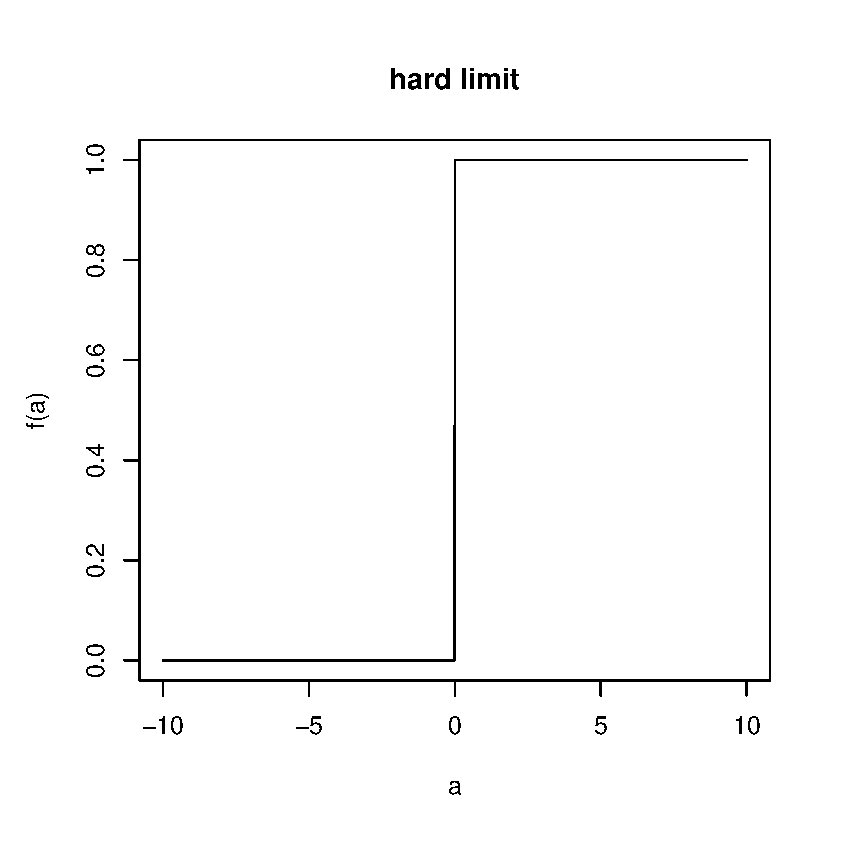
\includegraphics[height=3in]{04ANN/hardlim.eps}
%\end{center}
%\caption{ตัวอย่าง hard limit function ซึ่งเป็น activation function ของ perceptron: $f(a) = 1$ เมื่อ $a > 0$ และ $f(a) = 0$ เมื่อ $a < 0$.}
%\label{fig: ANN hard limit function}
%\end{figure}
%

ในตอนนั้น งานของโรเซนแบลททำให้วงการคอมพิวเตอร์ โดยเฉพาะอย่างยิ่งวงการปัญญาประดิษฐ์ตื่นเต้นมาก
ที่แนวทางนี้
อาจเป็นโอกาสที่มนุษย์จะสามารถสร้างเครื่องจักร
ที่สามารถเลียบแบบการทำงานของสมองมนุษย์ได้
และเป้าหมายของปัญญาประดิษฐ์ และความฝันของวิทยาการคอมพิวเตอร์อาจจะสำเร็จได้
เกิดการคาดการณ์ถึงศักยภาพ ความสามารถต่าง ๆ ที่เครื่องคอมพิวเตอร์จะสามารถทำได้.
แต่ความฝันและความหวังก็ล่มสลายไป 
หลังจาก มาร์วิน มินสกี้ (Marvin Minsky) และ เซมัวร์ ปาเปิต (Seymour Papert) ได้ร่วมกันเขียนหนังสือเพอร์เซปตรอนส์\cite{MinskyPapert1969a} ที่วิเคราะห์โครงสร้างและการทำงานของเพอร์เซปตรอน.
ประเด็นสำคัญของหนังสือ คือ
มินสกี้และปาเปิตถก และวิจารณ์ว่า
เพอร์เซปตรอนนั้นสามารถทำได้แต่งานง่าย ๆ 
เช่นหากเป็นงานการจำแนกประเภท ก็สามารถทำงานได้กับปัญหาที่สามารถแบ่งได้ด้วยเส้นแบ่งตัดสินใจเชิงเส้นเท่านั้น 
ไม่สามารถทำงานที่ซับซ้อนกว่านั้นได้.
\index{english}{linearly separable problem}
\index{thai}{ปัญหาที่สามารถแบ่งแยกได้เชิงเส้น}
พร้อมทั้งยังยกตัวอย่าง การทำงานของตรรกะ \textit{เอ็กซ์ออร์} (XOR หรือ exclusive OR) ที่เพอร์เซปตรอนไม่สามารถเลียบแบบได้.
ตาราง~\ref{tbl: ANN XOR} แสดงพฤติกรรมของตรรกะเอ็กซ์ออร์.

%
\begin{table}[hbtp]
	\caption[ตรรกะเอ็กซ์ออร์]{ตรรกะ\textit{เอ็กซ์ออร์} ที่อ้างว่าเพอร์เซปตรอน ไม่สามารถทำงานได้. 
	ตรรกะ\textit{เอ็กซ์ออร์} เป็นตรรกะ ที่ผลลัพธ์ไม่สามารถใช้เส้นแบ่งตัดสินใจเชิงเส้น มาตัดสินได้.}
	\begin{center}
		\begin{tabular}{|c|c|c|}
			\hline 
			$x_1$ & $x_2$ & $y$ \\
			\hline
			0     &    0  & 0   \\
			0     &    1  & 1   \\
			1     &    0  & 1   \\
			1     &    1  & 0   \\
			\hline
		\end{tabular} 
	\end{center}
	\label{tbl: ANN XOR}
\end{table}


ผลจากคำวิจารณ์ของมินสกี้และปาเปิต นอกจากจะทำให้เพอร์เซปตรอนเสื่อมความสนใจแล้ว 
ยังทำให้เทคนิคทางด้านโครงข่ายประสาทเทียมทั้งหมด รวมไปถึงสาขาวิชาปัญญาประดิษฐ์ 
เสียความนิยมและเสื่อมความสนใจไปในช่วงหลายปีต่อจากนั้น
จนเรียกกันว่า ช่วงเวลานั้นเป็น \textit{หน้าหนาวของปัญญาประดิษฐ์} (AI Winter).
%ช่วงนั้น ทุนวิจัย สำหรับงานด้านปัญญาประดิษฐ์ หาได้ยากมาก.
นอกจากคำวิจารณ์ของมินสกี้และปาเปิต
เหตุผลอื่น ๆ ที่มีส่วนทำให้โครงข่ายประสาทเทียมเสียความนิยมไป
ได้แก่
(1) การกำหนดโครงสร้างการเชื่อมต่อของโครงข่ายประสาทเทียม
ที่ตอนนั้นยังใหม่มาก และยังไม่มีแนวทางที่ชัดเจน%
\footnote{%
สถาปัตยกรรมที่ต่อหน่วยคำนวณย่อยเป็นลักษณะของชั้นคำนวณ ไม่ได้มาโดยธรรมชาติ แต่มาจากการออกแบบภายหลัง.
}
และ (2)
การใช้งานโครงข่ายประสาทเทียม
จะต้องเลือก\textit{ค่าน้ำหนัก}
และ\textit{ค่าไบอัส}ให้ถูกต้อง
ซึ่ง ณ ช่วงเวลานั้น
ยังไม่มีวิธีการที่มีประสิทธิภาพในการเลือก\textit{ค่าน้ำหนัก}
และ\textit{ค่าไบอัส}.
(ยังไม่มีแม้แต่ หลักในการเลือกจำนวนเพอร์เซปตรอนที่เหมาะสมกับการใช้งาน.)

จนกระทั่งราวทศวรรษให้หลัง งานของเวอร์โบส\cite{Werbos1974a}และโดยเฉพาะอย่างยิ่งงานของกลุ่มของรูเมลาร์ต ฮินตัน และวิลเลี่ยม\cite{RumelhartEtAl1986a} ที่ออกมาแสดงให้เห็นถึงประสิทธิผลของโครงข่ายประสาทเทียม 
พร้อมนำเสนอวิธีที่มีประสิทธิภาพ ในการหา\textit{ค่าน้ำหนัก}
และ\textit{ค่าไบอัส}
ซึ่งงานเหล่านี้ ได้ช่วยฟื้นฟูความนิยมของโครงข่ายประสาทเทียมกลับมาใหม่.

%
\begin{figure}
	\begin{center}
		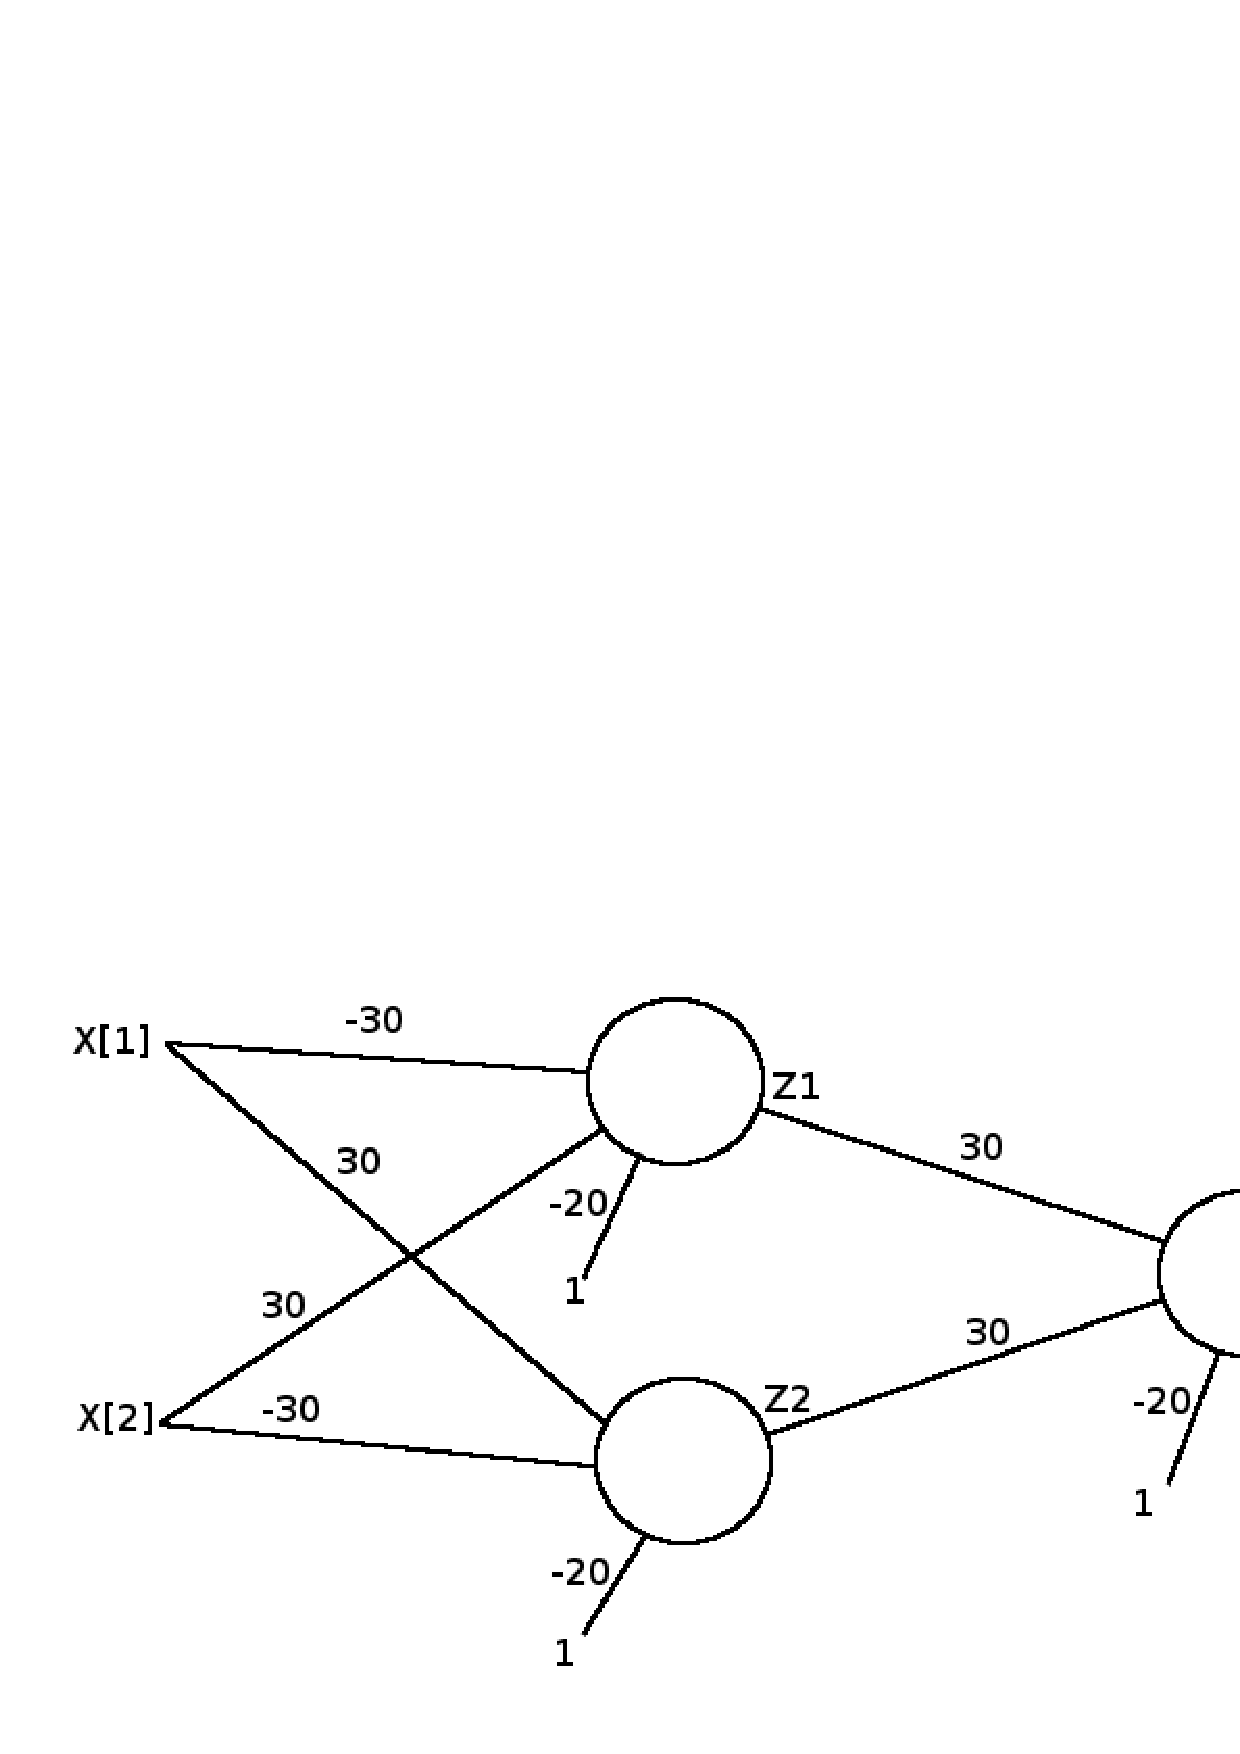
\includegraphics[height=2.5in]{03ANN/ann/MLPXor.png}
	\end{center}
	\caption[ตัวอย่างโครงข่ายเพอร์เซปตรอนสองชั้น]{ตัวอย่างโครงข่ายเพอร์เซปตรอนสองชั้น ที่ทำตรรกะเอ็กซ์ออร์. 
		เพอร์เซปตรอนสามหน่วยต่อในลักษณะชั้นคำนวณ โดย
		เพอร์เซปตรอนสองหน่วย รับอินพุต $x_1$ และ $x_2$
		และคำนวณเอาต์พุตออกมา เป็น $z_1$ (หน่วยบน) และ $z_2$ (หน่วยล่าง).
		เอาต์พุต $z_1$ และ $z_2$ จากสองหน่วย ถูกใช้เป็นอินพุตของเพอร์เซปตรอนตัวสุดท้าย (ตัวขวาสุด) 
		และเอาต์พุตของเพอร์เซปตรอนตัวสุดท้าย $y$ ถูกใช้เป็นเอาต์พุตของโครงข่าย.	
		ค่าน้ำหนักระหว่างการเชื่อมต่อ เขียนบริเวณเส้นแสดงการเชื่อมต่อ. 
		ในภาพ ค่า{ไบอัส} ถูกแสดงด้วยค่าน้ำหนักของอินพุตค่าคงที่หนึ่ง.}
	\label{fig: ANN MLP for XOR}
\end{figure}
%

เมื่อจะกล่าวไปแล้ว สิ่งที่มินสกี้กับปาเปิตวิจารณ์ว่า เพอร์เซปตรอนทำงานได้แต่งานง่าย ๆ ก็ไม่ได้ผิดซะทั้งหมด.
เพียงแต่ว่า มินสกี้กับปาเปิตสรุปความเห็น จากการวิเคราะห์การทำงานของ\textit{เพอร์เซปตรอน}ที่เป็นโครงข่ายชั้นเดียว.
การทำงานของโครงข่ายสมองมนุษย์ไม่ได้เป็นชั้นเดียว 
ในลักษณะเดียวกัน
โครงข่ายประสาทเทียมที่มีประสิทธิผล จะต้องมีโครงสร้างมากกว่าหนึ่งชั้น.
นั่นก็คือ ที่มาของพัฒนาการต่อมา ได้แก่ \textit{เพอร์เซปตรอนหลายชั้น} ซึ่งชื่อได้เน้นย้ำ
ถึงการใช้โครงข่ายต่อเชื่อมกันในลักษณะหลายชั้น
ของหน่วยคำนวณแบบเพอร์เซปตรอน.

รูป~\ref{fig: ANN MLP for XOR} แสดง\textit{เพอร์เซปตรอนสองชั้น} (two-layer perceptron) ที่สามารถเลียนแบบการทำงานของตรรกะเอ็กซ์ออร์ได้
โดยใช้เพอร์เซปตรอนสามตัว ต่อกันในลักษณะสองชั้นคำนวณ.
เพอร์เซปตรอนแต่ละตัว อาจถูกเรียกว่า
\textbf{โหนด} (node) หรือ \textbf{หน่วยคำนวณ} (unit).
\index{english}{node}
\index{english}{unit}
\index{thai}{โหนด}
\index{thai}{หน่วยคำนวณ}
ผลลัพธ์จากโหนดในชั้นคำนวณแรก
และส่งไปเป็นอินพุตให้กับโหนดในชั้นคำนวณที่สอง.
การจัดโครงสร้างเป็นลักษณะ\textbf{ชั้นคำนวณ} (layer) แบบนี้
\index{english}{layer}
\index{thai}{ชั้นคำนวณ}
ช่วยให้โครงข่ายประสาทเทียมสามารถทำงานที่ซับซ้อนได้.
เอาต์พุตของเพอร์เซปตรอนสองโหนดในชั้นแรก ซึ่งคือ $z_1 = h(-30 x_1 + 30 x_2 - 20)$ และ $z_2 = h(30 x_1 - 30 x_2 - 20)$
ทำหน้าที่เป็นอินพุตของเพอร์เซปตรอนตัวที่อยู่ชั้นที่สอง.
เอาต์พุตของเพอร์เซปตรอนชั้นที่สอง 
ซึ่งเป็นชั้นสุดท้าย ที่จะใช้เป็นเอาต์พุตของทั้งโครงข่าย
คำนวณด้วย $y = h(30 z_1 + 30 z_2 - 20)$.

ตาราง~\ref{tbl: ANN MLP for XOR} แจกแจงการทำงาน โดย $a^{(1)}_1$
และ $a^{(1)}_2$ เป็นตัวกระตุ้น (ผลรวมของสัญญาณกระตุ้น) ของโหนดตัวบน และของตัวล่างในชั้นที่หนึ่ง ตามลำดับ
และ $a^{(2)}$ เป็นของโหนดในชั้นที่สอง.
สังเกตว่า ค่าน้ำหนักและไบอัส
สามารถเปลี่ยนไปใช้ค่าอื่นได้ โดยที่การทำงานยังคงเดิมได้ 
เช่น อาจใช้ค่า $20, -20, -10$ แทน $30, -30, -20$ ในรูป~\ref{fig: ANN MLP for XOR} ได้ โดยพฤติกรรมการทำนายยังคงเดิม.
นี่เป็น
ลักษณะอย่างหนึ่งของโครงข่ายประสาทเทียม 
ที่ ค่าน้ำหนักและไบอัสที่ดีที่สุด มีได้หลายชุด.


%
\begin{table}[hbtp]
	\caption[ตัวอย่างการทำงานของเพอร์เซปตรอน]{การทำงานในแต่หน่วยของเพอร์เซปตรอน $2$ ชั้นในรูป~\ref{fig: ANN MLP for XOR}.
	แต่ละแถว แสดงแต่ละกรณี ตั้งแต่ $(x_1, x_2)$ เป็น $(0,0)$, $(0,1)$, $(1,0)$ และ $(1,1)$.
	สดมภ์ แสดงค่าของตัวแปรต่าง ๆ ดังระบุที่หัวสดมภ์ ได้แก่ อินพุต $x_1$ และ $x_2$,
ค่าการกระตุ้น $a_1$ และ $a_2$, ผลลัพธ์การกระตุ้น $z_1$ และ $z_2$ และเอาต์พุต $y$.	
}
	{\footnotesize	
%	{\small
		\begin{center}
			\begin{tabular}{|c|c|c|c|c|c|c|c|}
				\hline 
				$x_1$ & $x_2$ 
				& $a^{(1)}_1$ & $z_1$ 
				& $a^{(1)}_2$ & $z_2$ 
				& $a^{(2)}$ & $y$ \\
				\hline
				& & & & & & & \\
				$0$     &    $0$  
				& $-30 (0) + 30 (0) - 20$   & $h(-20)$
				& $30 (0) - 30 (0) - 20$   & $h(-20)$
				& $30 (0) + 30 (0) - 20$  & $h(-20)$ \\
				& 
				& $= -20$ & $= 0$
				& $= -20$ & $= 0$
				& $= -20$ &  $= 0$ \\
				\hline
				& & & & & & & \\
				$0$     &    $1$  
				& $-30 (0) + 30 (1) - 20$   & $h(10)$
				& $30 (0) - 30 (1) - 20$   & $h(-50)$
				& $30 (1) + 30 (0) - 20$  & $h(10)$ \\
				& 
				& $= 10$ & $= 1$
				& $= -50$ & $= 0$
				& $= 10$ &  $= 1$ \\
				\hline
				& & & & & & & \\				
				$1$     &    $0$  
				& $-30 (1) + 30 (0) - 20$   & $h(-50)$
				& $30 (1) - 30 (0) - 20$   & $h(10)$
				& $30 (1) + 30 (0) - 20$  & $h(10)$ \\
				& 
				& $= -50$ & $= 0$
				& $= 10$ & $= 1$
				& $= 10$ &  $= 1$ \\
				\hline
				& & & & & & & \\
				$1$     &    $1$  
				& $-30 (1) + 30 (1) - 20$   & $h(-20)$
				& $30 (1) - 30 (1) - 20$   & $h(-20)$
				& $30 (0) + 30 (0) - 20$  & $h(-20)$ \\
				& 
				& $= -20$ & $= 0$
				& $= -20$ & $= 0$
				& $= -20$ &  $= 0$ \\
				\hline
			\end{tabular} 
		\end{center}
	}%end /small
	\label{tbl: ANN MLP for XOR}
\end{table}



%\begin{minipage}{5.5in}
%{\small
%	\begin{shaded}
%		หากมองจากทฤษฎีการหาค่าดีที่สุด  
%		ปัญหาการหาค่าน้ำหนักที่ดีที่สุดของโครงข่ายประสาทเทียม จะเป็นปัญหาในลักษณะที่เรียกว่า \textit{ปัญหาที่ไม่เป็นคอนเวกซ์} (non-convex problem)
%		ซึ่งการหาค่าน้ำหนักที่ดีที่สุดในปัญหาแบบนี้จะทำได้ยาก.
%		%
%		ในทางปฏิบัติ การฝึกโครงข่ายประสาทเทียมก็คือการหาค่าน้ำหนักที่ดี 
%		แต่ไม่อาจรับประกันได้เลยว่าเราจะได้ค่าน้ำหนักที่ดีที่สุด 
%		ซึ่งเรื่องนี้เป็นลักษณะอย่างหนึ่งที่ผู้ใช้โครงข่ายประสาทเทียมมักสะท้อนออกมาว่า
%		%ให้ความเห็นว่า
%		โครงข่ายประสาทเทียมนั้นฝึกยาก
%	\end{shaded}
%}
%\end{minipage}


การคำนวณของโครงข่ายประสาทเทียม
แบบเพอร์เซปตรอนหลายชั้น สรุปได้ดังสมการ~\ref{eq: mlp feedforward x} ถึง~\ref{eq: mlp feedforward y}.
\begin{align}
z_j^{(0)} &= x_j &\mbox{สำหรับ }& j = 1, \ldots, D;
\label{eq: mlp feedforward x} \\ 
a_j^{(q)} &= \sum_i z_i^{(q-1)} \cdot w_{ji}^{(q)} + b_j^{(q)}
&\mbox{สำหรับ }& j = 1, \ldots, M_q;
\label{eq: mlp feedforward a} \\
z_j^{(q)} &= h(a_j^{(q)}) 
&\mbox{สำหรับ }& j = 1, \ldots, M_q;
\label{eq: mlp feedforward z} \\
\hat{y}_k &= z_k^{(L)}
&\mbox{สำหรับ }& k = 1, \ldots, K
\label{eq: mlp feedforward y} 
\end{align}
เมื่อ $q = 1, \ldots, L$ โดย $L$ เป็นจำนวนชั้นคำนวณ
และ
$\bm{x} = [x_1, \ldots, x_D]^T$ เป็นอินพุตของแบบจำลอง
และ $\bm{\hat{y}} = [\hat{y}_1, \ldots, \hat{y}_K]^T$ เป็นเอาต์พุตของแบบจำลอง.

ตัวแปร $a_j^{(q)}$ คือตัวกระตุ้นของโหนดที่ $j^{th}$ ในชั้นคำนวณที่ $q^{th}$.
การบวกในสมการ~\ref{eq: mlp feedforward a}
ทำสำหรับทุกโหนดในชั้นก่อนหน้า 
นั่นคือ $a_j^{(q)} = b_j^{(q)} + \sum_{i=1}^{M_{q-1}} z_i^{(q-1)} \cdot w_{ji}^{(q)}$
โดยกำหนด $M_0 = D$.
ชั้นคำนวณที่ $q^{th}$
มีโหนด จำนวน $M_q$ โหนด.
พารามิเตอร์ $w_{ji}^{(q)}$
เป็นค่าน้ำหนักสำหรับการเชื่อมต่อของโหนด $j^{th}$ ในชั้น $q^{th}$
กับโหนด $i^{th}$ ในชั้นก่อนหน้า.
พารามิเตอร์ $b_j^{(q)}$
เป็นค่าไบอัสของโหนด $j^{th}$ ในชั้น $q^{th}$.
ฟังก์ชัน $h$ เป็นฟังก์ชันกระตุ้น.

ตัวแปร $z_j^{(q)}$ เป็นเอาต์พุตของโหนด $j^{th}$ ในชั้น $q^{th}$ สำหรับ $q = 1, \ldots, L$
โดยสมการ~\ref{eq: mlp feedforward x} นิยามเอาต์พุตของชั้น $0^{th}$ เป็นอินพุตของแบบจำลอง เมื่อความกระทัดรัด.

เอาต์พุตของแบบจำลองคือ
เอาต์พุตของโหนดต่าง ๆ ในชั้นสุดท้าย (ดังระบุในสมการ~\ref{eq: mlp feedforward y})
ดังนั้น $M_L = K$ โดย $K$ เป็นจำนวนมิติของเอาต์พุตที่ต้องการ.
จำนวนชั้นคำนวณ 
และจำนวนโหนดในแต่ละชั้น
เป็น
\textit{อภิมานพารามิเตอร์}
\index{thai}{อภิมานพารามิเตอร์}
\index{english}{meta-parameter}
\index{english}{hyper-parameter}
ของแบบจำลองเพอร์เซปตรอนหลายชั้น.

สมการ~\ref{eq: mlp feedforward x} ถึง~\ref{eq: mlp feedforward y}
แสดงการคำนวณของเพอร์เซปตรอน
ในรูปตัวแปรสเกล่าร์.
การคำนวณของเพอร์เซปตรอน
สามารถเขียนได้กระชับกว่า
โดยเขียนในรูปเวกเตอร์และเมทริกซ์
ดังสมการ~\ref{eq: mlp feedforward a vec}
และ~\ref{eq: mlp feedforward z vec} 
ซึ่ง การจัดรูปในลักษณะนี้จะเรียกว่า
\textbf{เวคตอไรเซชั่น} (vectorization).
\index{english}{vectorization}
\index{thai}{เวคตอไรเซชั่น}
\begin{align}
\bm{a}^{(q)} &=   \bm{W}^{(q)} \cdot \bm{z}^{(q-1)} + \bm{b}^{(q)}
\label{eq: mlp feedforward a vec} \\
\bm{z}^{(q)} &= h(\bm{a}^{(q)})
\label{eq: mlp feedforward z vec}
\end{align}
สำหรับ $q = 1, \ldots, L$
เมื่อ $L$ คือจำนวนชั้นคำนวณ.
ตัวแปร $\bm{a}^{(q)} = [a^{(q)}_1, \;a^{(q)}_2, \ldots, \; a^{(q)}_{M_q}]^T$ คือตัวกระตุ้นของชั้นคำนวณ $q^{th}$
ที่มี $M_q$ โหนด.
ตัวแปร $\bm{z}^{(q)} = [z^{(q)}_1, \;z^{(q)}_2, \ldots, \; z^{(q)}_{M_q}]^T$ คือ ผลลัพธ์การกระตุ้นในชั้นคำนวณ $q^{th}$
โดยกำหนดให้
อินพุตเสมือนมาจากโหนดชั้นศูนย์ นั่นคือ
$\bm{z}^{(0)}  = \bm{x} = [x_1, \ldots, x_D]^T$
และเอาต์พุตของระบบ
$[\hat{y}_1, \ldots, \hat{y}_K]^T = \bm{\hat{y}} \equiv \bm{z}^{(L)}$.
เมทริกซ์ $\bm{W}^{(q)} \in \mathbb{R}^{M_q \times M_{q-1}}$
และเวกเตอร์ $\bm{b}^{(m)} \in \mathbb{R}^{M_q}$
คือค่าน้ำหนักและค่าไบอัสของชั้นคำนวณ $q^{th}$
และ $M_0 = D$ และ $M_L = K$.
ฟังก์ชัน $h$ เป็นฟังก์ชันกระตุ้น
ซึ่งสำหรับฟังก์ชันกระตุ้น $h: \mathbb{R} \mapsto \mathbb{R}$
นิยามสัญกรณ์ เช่น $h(\bm{a})$ เป็นปฏิบัติการที่มีลักษณะการคำนวณ\textit{เชิงตัวต่อตัว} (element-wise) เมื่อใช้กับเวกเตอร์ เมทริกซ์ หรือเทนเซอร์ (ยกเว้นจะระบุเป็นอย่างอื่น).
นั่นคือ เช่น $h([a_1, \ldots, a_m]^T) =[h(a_1), \ldots, h(a_m)]^T$.

สังเกตว่า
การคำนวณจะดำเนินการในลักษณะคล้าย ๆ กัน
เป็น\textit{ชั้นคำนวณ} \index{english}{layer}
\index{thai}{ชั้นคำนวณ}
อินพุตของระบบถูกป้อนให้กับชั้นคำนวณแรก
เมื่อคำนวณผลจากชั้นหนึ่งเสร็จแล้ว ผลลัพธ์จะถูกใช้ป้อนเป็นอินพุตให้กับชั้นคำนวณต่อไป และดำเนินการเช่นนี้ต่อไปจนถึงชั้นคำนวณสุดท้าย
ผลลัพธ์ของชั้นคำนวณสุดท้าย จะใช้เป็นเอาต์พุตของระบบ.
เนื่องจากการคำนวณมีลักษณะที่คำนวณเป็นชั้น ๆ ผ่านไปทิศทางเดียว 
\textit{เพอร์เซปตรอนหลายชั้น}
บางครั้งอาจถูกเรียกว่า \textbf{โครงข่ายแพร่กระจายไปข้างหน้า} (feedforward network)
\index{english}{feedforward network}
\index{thai}{โครงข่ายแพร่กระจายไปข้างหน้า}.
ชั้นคำนวณทั้งหมดที่อยู่ก่อนชั้นสุดท้าย
นั่นคือ ชั้น $q = 1, \ldots, L-1$
จะเรียกว่า \textbf{ชั้นซ่อน} (hidden layer)
\index{english}{hidden layer}
\index{thai}{ชั้นซ่อน}
เนื่องจากเอาต์พุตของชั้นคำนวณเหล่านี้
ไม่ได้ใช้เป็นเอาต์พุตสุดท้ายของแบบจำลอง
และโหนดต่าง ๆ ที่อยู่ใน\textit{ชั้นซ่อน} จะเรียกว่า \textbf{โหนดซ่อน} (hidden node) หรือ \textbf{หน่วยซ่อน} (hidden unit).
\index{english}{hidden node}
\index{english}{hidden unit}
\index{thai}{หน่วยซ่อน}
\index{thai}{โหนดซ่อน}
การเลือก\textit{อภิมานพารามิเตอร์}ของเพอร์เซปตรอนหลายชั้น
บางครั้งนิยม อ้างถึงจำนวนชั้นซ่อน เช่นในตัวอย่างรูป~\ref{fig: ANN perceptron} อาจอ้างถึงเป็น
โครงข่ายประสาทเทียม หนึ่งชั้นซ่อน ที่มีสองหน่วยซ่อน.
หมายเหตุ ถึงแม้โครงข่ายประสาทเทียม
จะมีหลายชนิด
แต่เพอร์เซปตรอนหลายชั้น เป็นชนิดแรก และเป็นชนิดที่รู้จักกันอย่างกว้างขวาง
บ่อยครั้งที่ 
คำว่า 
\textit{เพอร์เซปตรอนหลายชั้น},
\textit{โครงข่ายประสาทเทียม}
หรือ\textit{โครงข่ายแพร่กระจายไปข้างหน้า} ถูกใช้แทนกัน.

%
ปัจจุบันโครงข่ายประสาทเทียม
เป็นแบบจำลองได้ถูกนำไปใช้อย่างกว้างขวาง ในงานหลาย ๆ ลักษณะ เช่น การหาค่าถดถอย การจำแนกประเภท การประมาณฟังก์ชัน. 
%และใช้เป็นส่วนประกอบภายในแอพพลิเคชั่นต่าง ๆ อย่างกว้างขวาง. 
%
นอกจากนั้น มีการศึกษาโครงข่ายประสาทเทียมในทางทฤษฎี และพิสูจน์ว่าโครงข่ายประสาทเทียม
เป็น\textit{ตัวประมาณค่าสากล} (universal approximator)\cite{Cybenko1989a, Hornik1991a}
\index{english}{universal approximator}
\index{thai}{ตัวประมาณค่าสากล}
ซึ่งความหมายคือ 
โครงข่ายประสาทเทียม
สามารถแทนฟังก์ชันใด ๆ ก็ได้ ที่ความละเอียดตามที่ต้องการ หากมีจำนวนหน่วยคำนวณมากเพียงพอ.
ตามทฤษฎีแล้ว แค่โครงข่ายประสาทเทียมแบบสองชั้น
ก็เป็นตัวประมาณค่าสากลได้แล้ว
แต่การใช้โครงข่ายประสาทเทียมแบบลึก
มีประโยชน์หลายอย่าง
ดังที่จะอภิปรายในบทที่~\ref{chapter: Deep Learning}.
%
%อภิปรายโครงข่ายประสาทเทียมแบบลึก ที่ลึกมากกว่าสองชั้น และประโยชน์.
%ก็สามารถที่ จะแทนฟังก์ชันใด ๆ ได้แล้ว หากมีจำนวนเพอร์เซปตรอนใน ชั้นที่ซ่อนไว้มากเพียงพอ.
%
%โครงข่ายประสาทเทียม $2$ ชั้น สามารถประมาณแทนฟังก์ชันได้ทุกชนิด ในความละเอียดตามที่ต้องการได้ เพียงต้องมีจำนวน หน่วยประสาทเทียมที่มากเพียงพอเท่านั้น.



\subsection{การฝึกโครงข่ายประสาทเทียม}
\label{sec: ann training}
\index{thai}{การฝึก}
\index{thai}{การฝึก!โครงข่ายประสาทเทียม}
\index{thai}{โครงข่ายประสาทเทียม!การฝึก}
\index{english}{train}
\index{english}{artificial neural network!train}
\index{english}{train!artificial neural network}

กลับมาที่เรื่องการหา\textit{ค่าน้ำหนัก}และ\textit{ค่าไบอัส}ที่เหมาะสม
อย่างที่เห็นจากตัวอย่าง การที่โครงข่ายประสาทเทียมจะสามารถทำงานได้ตามที่ต้องการนั้น 
นอกจากโครงข่ายจะต้องมีโครงสร้างที่รองรับได้แล้ว
(โครงสร้างเป็นลักษณะชั้น ๆ ต่อกันที่เหมาะสม และมีจำนวนหน่วยคำนวณเพียงพอ) 
\textit{ค่าน้ำหนัก}และ\textit{ค่าไบอัส}ต่าง ๆ
จะต้องมีค่าที่เหมาะสมด้วย.

\textit{ค่าน้ำหนัก}และ\textit{ค่าไบอัส}
ของ\textit{โครงข่ายประสาทเทียม}
ก็คือ \textit{พารามิเตอร์}ต่าง ๆ ของแบบจำลอง.
ดังนั้น 
การหา\textit{ค่าน้ำหนัก}และ\textit{ค่าไบอัส}
ก็สามารถทำได้ในลักษณะเดียวกับ การหาค่าพารามิเตอร์ของฟังก์ชันพหุนามที่ได้อภิปรายในหัวข้อ~\ref{sec: curve fitting}.
นั่นคือ
การใช้วิธีของการหาค่าดีที่สุด
และเช่นเดียวกัน
การหา\textit{ค่าน้ำหนัก}และ\textit{ค่าไบอัส}
จะเรียกว่า \textit{การฝึก}.

อย่างไรก็ตาม 
เปรียบเทียบการฝึกแบบจำลองพหุนาม
กับการฝึกโครงข่ายประสาทเทียม
มีประเด็นที่น่าสนใจ คือ
อนุพันธ์ของฟังก์ชันจุดประสงค์ต่อค่าพารามิเตอร์.
การหาอนุพันธ์
เป็นกลไกสำคัญ
สำหรับวิธีของการหาค่าดีที่สุดอย่างมีประสิทธิภาพ.
เพอร์เซปตรอนใช้\textit{ฟังก์ชันจำกัดแข็ง}
เป็นฟังก์ชันกระตุ้น
แต่เนื่องจาก \textit{ฟังก์ชันจำกัดแข็ง} (สมการ~\ref{eq: ANN hard limit}) เป็นฟังก์ชันที่มีค่าไม่ต่อเนื่อง (ที่ $a = 0$) 
ทำให้ไม่สามารถหาค่าอนุพันธ์ของ\textit{ฟังก์ชันจำกัดแข็ง}
และส่งผลให้การหาค่าน้ำหนักที่เหมาะสมของเพอร์เซปตรอนทำได้ยาก.

\textit{ฟังก์ชันจำกัดแข็ง} แม้จะเลียนแบบการทำงานของเซลล์ประสาท แต่ลักษณะทางคณิตศาสตร์ของมัน
เป็นอุปสรรคสำคัญ
ต่อการฝึกโครงข่ายประสาทเทียม.
การสร้างแบบจำลองคณิตศาสตร์
เพื่อทำความเข้าใจเซลล์ประสาทชีวภาพ 
จัดอยู่ในขอบข่ายของ\textit{ประสาทวิทยาเชิงคำนวณ} (computational neuroscience) 
ซึ่งเป็นสาขาเฉพาะ และอยู่นอกเหนือจากขอบเขตของหนังสือเล่มนี้.
%
แม้กระนั้น \textit{ฟังก์ชันจำกัดแข็ง}
ก็ไม่ได้อธิบายการทำงานของเซลล์ประสาทชีวภาพได้เที่ยงตรงซะทีเดียว
นอกจากนั้น สิ่งที่ต้องการจริง ๆ ในมุมมองทางวิศวกรรม ก็คือเครื่องมือที่ใช้งานได้ เช่น แบบจำลองที่มีความสามารถในการทำนายที่ดี.
%ดังนั้นจึงไม่มีเหตุผล ที่จะยึดติดกับฟังก์ชันจำกัดแข็ง.

การฝึกโครงข่ายประสาทเทียมที่ใช้\textit{ฟังก์ชันจำกัดแข็ง}จะทำได้ยาก
และไม่สามารถทำได้อย่างมีประสิทธิภาพ.
%
เมื่อปัญหาอยู่ที่\textit{ฟังก์ชันจำกัดแข็ง} 
วิธีแก้ก็แก้ที่\textit{ฟังก์ชันจำกัดแข็ง}.
สิ่งที่รูเมลาร์ต ฮินตัน และวิลเลี่ยม\cite{RumelhartEtAl1986a} เสนอคือ ใช้\textbf{ฟังก์ชันซิกมอยด์} (sigmoid function หรือบางครั้งเรียก logistic function หรือ logistic sigmoid function)
เป็นฟังก์ชันกระตุ้น แทน\textit{ฟังก์ชันจำกัดแข็ง}.
สมการ~\ref{eq: sigmoid} แสดงการคำนวณ\textit{ฟังก์ชันซิกมอยด์}
\begin{eqnarray}
\mathrm{sigmoid}(a) = \frac{1}{1 + \exp(-a)}
\label{eq: sigmoid}.
\end{eqnarray}
\index{english}{sigmoid}
\index{english}{function!sigmoid}
\index{thai}{ฟังก์ชันซิกมอยด์}
\index{thai}{ฟังก์ชัน!ซิกมอยด์}
\index{english}{activation!sigmoid}
\textit{ฟังก์ชันซิกมอยด์} เป็นฟังก์ชันค่าต่อเนื่อง ดังนั้นจึงสามารถหาอนุพันธ์ได้.
รูป~\ref{fig: ANN activation function} แสดงค่าผลลัพธ์การกระตุ้นจาก\textit{ฟังก์ชันจำกัดแข็ง}เปรียบเทียบกับ\textit{ฟังก์ชันซิกมอยด์}.


อย่างไรก็ตามแม้ ชื่อของเพอร์เซปตรอนจะเชื่อมโยงกับ\textit{ฟังก์ชันจำกัดแข็ง}
แต่ในทางปฏิบัติแล้ว 
โดยทั่วไป
ชื่อ\textit{เพอร์เซปตรอนหลายชั้น} ก็มักอ้างถึงโครงข่ายประสาทเทียม
ที่ใช้\textit{ฟังก์ชันซิกมอยด์}เป็นฟังก์ชันกระตุ้น.
นอกจาก\textit{ฟังก์ชันซิกมอยด์}แล้ว
\textbf{ฟังก์ชันไฮเปอร์บอลิกแทนเจนต์} (hyperbolic tangent function)
ซึ่งคำนวณโดย
$\tanh(x) = (e^x - e^{-x})/(e^x + e^{-x})$ 
\index{english}{hyperbolic tangent}
\index{english}{tanh}
\index{english}{activation!tanh}
ก็นิยมใช้เป็นฟังก์ชันกระตุ้นของโครงข่ายประสาทเทียม.

%
\begin{figure}
	\begin{center}
		\includegraphics[height=2in]{03ANN/ann/hardlim_sigmoid.png}
	\end{center}
	\caption[ฟังก์ชันจำกัดแข็งกับฟังก์ชันซิกมอยด์]{ภาพเปรียบเทียบฟังก์ชันจำกัดแข็ง (เส้นบางสีฟ้า) กับฟังก์ชันซิกมอยด์ (เส้นหนาสีแดง).}
	\label{fig: ANN activation function}
\end{figure}
%

อีกประเด็น
ฟังก์ชันกระตุ้น $h$ ในสมการ~\ref{eq: mlp feedforward z} หรือ~\ref{eq: mlp feedforward z vec}
ไม่จำเป็นต้องใช้เหมือนกันทุก ๆ ชั้นคำนวณ.
นั่นคือ สมการ~\ref{eq: mlp feedforward z vec} อาจเขียนใหม่ เพื่อเน้นประเด็นนี้ ได้เป็น $\bm{z}^{(q)} = h_q(\bm{a}^{(q)})$
เมื่อ $h_q$ เป็นฟังก์ชันกระตุ้นของชั้น $q^{th}$.
ในทางปฏิบัติแล้ว
ฟังก์ชันกระตุ้นของชั้นคำนวณสุดท้าย
มักจะต่างจากฟังก์ชันกระตุ้นของชั้นอื่น ๆ.
ชั้นคำนวณสุดท้าย มักถูกเรียกว่า
\textbf{ชั้นเอาต์พุต} (output layer)
\index{thai}{ชั้นเอาต์พุต}
\index{english}{output layer}
เป็นชั้นที่จะเตรียมค่าของเอาต์พุต
ให้อยู่ในรูปแบบที่ใกล้เคียง
กับรูปแบบเอาต์พุตที่เหมาะสมกับภารกิจมากที่สุด.
%
ฟังก์ชันกระตุ้นของชั้นเอาต์พุต เรียกสั้น ๆ ว่า 
\textbf{ฟังก์ชันกระตุ้นเอาต์พุต} (output activation function)
\index{thai}{ฟังก์ชันกระตุ้นเอาต์พุต}
\index{english}{output activation function}
จะถูกเลือกใช้ตามภาระกิจ และลักษณะค่าเอาต์พุตที่ต้องการ.
ตัวอย่างเช่น
\textit{การหาค่าถดถอย} ซึ่งต้องการเอาต์พุต $y \in \mathbb{R}$.
	\index{english}{regression}
	\index{thai}{การหาค่าถดถอย}
	\index{english}{task!regression}
	\index{thai}{ภารกิจ!การหาค่าถดถอย}
	%
	ฟังก์ชันกระตุ้นเอาต์พุต นิยมใช้\textit{ฟังก์ชันเอกลักษณ์} (identity function).
	นั่นคือ $h(a) = a$.
\index{thai}{ฟังก์ชันกระตุ้นเอาต์พุต!ฟังก์ชันเอกลักษณ์}
\index{english}{output activation function!identity function}
	
เมื่อเลือกใช้ฟังก์ชันกระตุ้นเป็นฟังก์ชันต่อเนื่องแล้ว
การฝึกโครงข่ายประสาทเทียม
ก็สามารถทำได้อย่างมีประสิทธิภาพ
โดยอาศัยค่าอนุพันธ์.
เช่นเดียวกับแบบจำลองทำนายอื่น ๆ
การฝึกโครงข่ายประสาทเทียม
คือ การหา
$\bm{\Theta}^\ast = \arg\min_{\bm{\Theta}} E$
เมื่อ 
$E$ คือ ฟังก์ชันค่าผิดพลาดที่เป็นจุดประสงค์
และ
$\bm{\Theta}$ คือพารามิเตอร์ของแบบจำลอง ซึ่งสำหรับโครงข่ายประสาทเทียม จากสมการ~\ref{eq: mlp feedforward a} ก็คือ 
%$\bm{\Theta} = \{ \bm{W}^{(1)},  \bm{b}^{(1)}, \ldots, \bm{W}^{(L)},  \bm{b}^{(L)} \}$.
$\bm{\Theta} = \{ w_{ji}^{(q)}, b_j^{(q)} \}$
โดย $q=1,\ldots,L;$ 
$j=1, \ldots, M_q;$ 
และ $i = 1, \ldots, M_{q-1}$.
%
%หมายเหตุ
%สัญกรณ์ เช่น $\{v_i\}_{i=1,\ldots,M}$ หมายถึงเซต $\{v_1, \; v_2, \; v_3, \; \ldots, \; v_M\}$.

สำหรับงาน\textbf{การหาค่าถดถอย} (regression)
\index{thai}{การหาค่าถดถอย}
\index{english}{regression}
ซึ่งคือการทำนายเอาต์พุตที่ค่าเป็นจำนวนจริง
ฟังก์ชันค่าผิดพลาด $E$
สามารถนิยามด้วย \textit{ค่าเฉลี่ยค่าผิดพลาดกำลังสอง}
\index{english}{loss!mean square error}
\index{thai}{ฟังก์ชันสูญเสีย!ค่าเฉลี่ยค่าผิดพลาดกำลังสอง}
ดังแสดงในสมการ~\ref{eq: ann E} สำหรับข้อมูลจำนวน $N$ จุดข้อมูล.
\begin{align}
E =& \frac{1}{N}\sum_{n=1}^N E_n
\label{eq: ann E} \\
E_n =& \frac{1}{2} \|\bm{\hat{y}}(\bm{x}_n, \bm{\Theta}) - \bm{y}(n)\|^2
\label{eq: ann En}
\end{align}
เมื่อ $\bm{y}(n)$ คือ\textit{เฉลย} หรือค่า\textit{ตัวแปรตาม}จากจุดข้อมูลที่ $n^{th}$
และ $\bm{\hat{y}}(\bm{x}_n, \bm{\Theta})$ ที่อาจเขียนย่อเป็น $\bm{\hat{y}}$ หากบริบทชัดเจน
คือค่าที่แบบจำลองทำนายสำหรับจุดข้อมูลที่ $n^{th}$ เมื่อใช้ค่าพารามิเตอร์เป็น $\bm{\Theta}$.
ค่าของ
$\bm{\hat{y}} = \bm{z}^{(L)}$ 
คำนวณได้จากสมการ~\ref{eq: mlp feedforward a vec}
และ~\ref{eq: mlp feedforward z vec}
โดยให้ $\bm{z}^{(0)} = \bm{x}_n$ 
เมื่อ $\bm{x}_n$
เป็นค่า\textit{ตัวแปรต้น}ของจุดข้อมูลที่ $n^{th}$.

การหา
$\bm{\Theta}^\ast = \arg\min_{\bm{\Theta}} E$
ที่มีประสิทธิภาพ ต้องการค่าเกรเดียนต์ $\nabla_{\Theta} E = \frac{1}{N} \sum_{n=1}^N \nabla_{\Theta} E_n$ ซึ่งสามารถพิจารณาได้จาก
%เกรเดียนต์ 
\begin{align}
\nabla_{\Theta} E_n =& 
\begin{bmatrix}
\frac{\partial E_n}{\partial w_{1,1}^{(1)}}
& \ldots &
%\frac{\partial E_n}{\partial w_{1,M_0}^{(1)}}
%& \ldots &
\frac{\partial E_n}{\partial w_{M_1,M_0}^{(1)}}
&
\frac{\partial E_n}{\partial b_1^{(1)}}
& \ldots &
\frac{\partial E_n}{\partial b_{M_1}^{(1)}}
& \ldots &
\frac{\partial E_n}{\partial w_{M_L,M_{L-1}}^{(L)}}
& \ldots &
\frac{\partial E_n}{\partial b_{M_L}^{(L)}}
\end{bmatrix}^T
\label{eq: backprop grad dEn}
\end{align}
หรืออาจเขียนย่อ ๆ เป็น
$\nabla_{\Theta} E_n = \left[ \frac{\partial E_n}{\partial w_{ji}^{(q)}}, \; \frac{\partial E_n}{\partial b_j^{(q)}} \right]^T$
โดย $q=1,\ldots,L;$ 
$i=1,\ldots,M_{q-1};$
และ $j=1,\ldots,M_q$.

พิจารณาแต่ละส่วนประกอบของเกรเดียนต์ 
จากกฎลูกโซ่ของการหาอนุพันธ์
$\frac{\partial E_n}{\partial w_{ji}^{(q)}} =
\frac{\partial E_n}{\partial a_j^{(q)}} \cdot
\frac{\partial a_j^{(q)}}{\partial w_{ji}^{(q)}}$
เพื่อความกระชับ
สัญกรณ์ที่แสดง อาจละตัวยก $\;^{(q)}$ ในกรณีที่บริบทชัดเจน
นั่นคือ อนุพันธ์ดังกล่าวจะเขียนเป็น
\begin{align}
\frac{\partial E_n}{\partial w_{ji}} 
& =
\frac{\partial E_n}{\partial a_j} \cdot
\frac{\partial a_j}{\partial w_{ji}}
&
\mbox{และ} &&
\frac{\partial E_n}{\partial b_j} & =
\frac{\partial E_n}{\partial a_j} \cdot
\frac{\partial a_j}{\partial b_j}
\label{eq: backprop dE/dw}
\end{align}

กำหนดให้ $\delta_j^{(q)} \equiv \frac{\partial E_n}{\partial a_j^{(q)}}$ และเมื่อบริบทชัดเจน อาจเขียนย่อเป็น
\begin{align}
\delta_j \equiv &
\frac{\partial E_n}{\partial a_j}
\label{eq: backprop delta}.
\end{align}

จากสมการ~\ref{eq: mlp feedforward a} นั่นคือ $a_j = \sum_i z_i^{(q-1)} \cdot w_{ji} + b_j$ 
ดังนั้น
\begin{align}
\frac{\partial a_j}{\partial w_{ji}}
&
= z_i^{(q-1)}
&
\mbox{และ} &&
\frac{\partial a_j}{\partial b_j} &
= 1
\label{eq: backprop da/dw}
\end{align}
เมื่อแทนสมการ~\ref{eq: backprop da/dw} ลงในสมการ~\ref{eq: backprop dE/dw} จะได้
\begin{align}
\frac{\partial E_n}{\partial w_{ji}^{(q)}}
&
= \delta_j^{(q)} \cdot z_i^{(q-1)}
&
\mbox{และ} &&
\frac{\partial E_n}{\partial b_j^{(q)}} &
= \delta_j^{(q)}
\label{eq: backprop dE/dw in delta}.
\end{align}

พิจารณา $\delta_j^{(q)} = \frac{\partial E_n}{\partial a_j^{(q)}}$ ที่ชั้นเอาต์พุต $q = L$
แทนค่า $E_n$ จากสมการ~\ref{eq: ann En} และสำหรับ\textit{การหาค่าถดถอย} \textit{ฟังก์ชันกระตุ้นเอาต์พุต}ใช้\textit{ฟังก์ชันเอกลักษณ์} นั่นคือ $[\hat{y}_1, \; \ldots, \; \hat{y}_K]^T = [a_1^{(L)}, \; \ldots, \; a_K^{(L)}]^T$
จะได้ว่า
$\delta_k^{(L)} = \frac{\partial E_n}{\partial a_k^{(L)}}$
$= \frac{\partial \frac{1}{2} \sum_m (\hat{y}_m - y_m)^2}{\partial a_k^{(L)}}$
และหลังจากหาอนุพันธ์จะได้
\begin{align}
\delta_k^{(L)}
&
= \hat{y}_k - y_k
\label{eq: backprop delta L}.
\end{align}
ที่ชั้นซ่อน $q < L$ 
ตัวกระตุ้น $a_j^{(q)}$ จะส่งผลต่อ $E_n$ ผ่านโหนดต่าง ๆ ในชั้นถัดไป (รูป~\ref{fig: backpropagation})
ดังนั้น
จากกฎลูกโซ่ของการหาอนุพันธ์
\begin{align}
\delta_j^{(q)} &
= \frac{\partial E_n}{\partial a_j^{(q)}}
= 
\sum_m \frac{\partial E_n}{\partial a_m^{(q+1)}} \cdot \frac{\partial a_m^{(q+1)}}{\partial a_j^{(q)}}
\label{eq: backprop dE/da chain rule}.
\end{align}
พจน์หน้า $\frac{\partial E_n}{\partial a_m^{(q+1)}} = \delta_m^{(q+1)}$
มาจากชัดถัดไป.
พจน์หลังคำนวณได้โดยเขียน $a_m^{(q+1)}$
จากสมการ~\ref{eq: mlp feedforward a} และ~\ref{eq: mlp feedforward z}
และหาอนุพันธ์
ซึ่งผลลัพธ์คือ
$\frac{\partial a_m^{(q+1)}}{\partial a_j^{(q)}}$
%$= \frac{\partial \sum_k w_{mk}^{(q+1)} z_k^{(q)} + b_m^{(q+1)}}{\partial a_j^{(q)}}$
%$= w_{mj}^{(q+1)} \frac{\partial z_j^{(q)}}{\partial a_j^{(q)}}$
$= w_{mj}^{(q+1)} \frac{\partial h(a_j^{(q)})}{\partial a_j^{(q)}}$.
แทนทั้งสองพจน์นี้ในสมการ~\ref{eq: backprop dE/da chain rule} แล้วจะได้ว่า สำหรับชั้นซ่อน ($q < L$)
แล้ว
\begin{align}
\delta_j^{(q)} 
& = h'(a_j^{(q)}) \cdot \sum_m \delta_m^{(q+1)} \cdot w_{mj}^{(q+1)}
\label{eq: backprop delta q < L}
\end{align}
เมื่อ $h'(a_j^{(q)}) = \frac{\partial h(a_j^{(q)})}{\partial a_j^{(q)}}$ คืออนุพันธ์ของฟังก์ชันกระตุ้น
ที่ค่า $a_j^{(q)}$.
หมายเหตุ  $h'(a_j^{(q)})$ เป็นอนุพันธ์ของฟังก์ชันกระตุ้นของชั้น $q^{th}$
และบางครั้ง
อาจใช้สัญกรณ์ $h_q'(a_j^{(q)}) = \frac{\partial h_q(a_j^{(q)})}{\partial a_j^{(q)}}$
ในกรณีที่อาจสับสน.

ทั้งหมดที่อภิปรายมา
สรุปได้ว่า
เกรเดียนต์ของโครงข่ายประสาทเทียม
$\nabla_{\Theta} E_n$ สามารถหาได้โดยกระบวนการดังนี้
\begin{enumerate}
	\item ทำ\textit{การคำนวณไปข้างหน้า} (forward propagation หรือ forward pass) โดยคำนวณสมการ~\ref{eq: mlp feedforward x} ถึง~\ref{eq: mlp feedforward y}.
	สิ่งที่ได้คือ ค่าที่ทำนาย $\bm{\hat{y}}$ กับ ค่าตัวกระตุ้นและผลลัพธ์การกระตุ้นต่าง ๆ $\bm{a}^{(q)}$ และ $\bm{z}^{(q)}$ สำหรับ $q = 1, \ldots, L$.
 	\item คำนวณค่า $\delta_k^{(L)}$ สำหรับทุก ๆ โหนดเอาต์พุต $k = 1, \ldots, K$ ตามสมการ~\ref{eq: backprop delta L}.
 	สิ่งที่ได้คือ $\bm{\delta}^{(L)}$.
 	\item คำนวณค่า $\delta_j^{(q)}$ สำหรับทุก ๆ โหนด ในทุก ๆ ชั้นซ่อน $j = 1,\ldots,M_q; q = 1, \ldots, L-1$ ตามสมการ~\ref{eq: backprop delta q < L}.
 	สิ่งที่ได้คือ $\bm{\delta}^{(q < L)}$.
 	\item คำนวณค่าอนุพันธ์ที่ต้องการ จากสมการ~\ref{eq: backprop dE/dw in delta}.
 	สิ่งที่ได้คือ $\frac{\partial E_n}{\partial w_{ji}}$ 
 	และ $\frac{\partial E_n}{\partial b_j}$
 	ค่าต่าง ๆ ทุกค่า ซึ่งรวมกันเป็นเกรเดียนต์ $\nabla_{\Theta} E_n$.
\end{enumerate}

เกรเดียนต์ $\nabla_{\Theta} E_n$ ที่ได้สามารถนำไปใช้กับ\textit{ขั้นตอนวิธีการหาค่าดีที่สุด} (optimization algorithm) เช่น \textit{วิธีลงเกรเดียนต์}ที่อภิปรายในหัวข้อ~\ref{sec: optimization} ได้.
กระบวนการหาเกรเดียนต์ $\nabla_{\Theta} E_n$ ที่ได้อภิปรายมานี้ คือ วิธี\textbf{การแพร่กระจายย้อนกลับ} (error backpropagation หรือ backpropagation)
\index{thai}{การแพร่กระจายย้อนกลับ}
\index{english}{backpropagation}
\index{english}{train!backpropagation}
คณะของ
ที่รูเมลาร์ต\cite{RumelhartEtAl1986a} เสนอในปี ค.ศ. 1986
และเป็นการค้นพบที่ฟื้นฟูความสนใจในโครงข่ายประสาทเทียมกลับมา หลังจากกว่าทศวรรษของ\textit{หน้าหนาวของปัญญาประดิษฐ์}.


%
\begin{figure}[H]
	\begin{center}
		\includegraphics[width=3.0in]
		{03Ann/ann/backprop.png}
	\end{center}
	\caption[ผลจากโหนดที่ส่งผ่านโหนดอื่น ๆ ในชั้นคำนวณถัดไป]{ภาพแสดงการเชื่อมต่อ และเน้นผลของโหนด $j^{th}$ ในชั้น $q^{th}$ ที่มีต่อค่าผิดพลาด
	โดยผ่านโหนดต่าง ๆ ในชั้น $(q+1)^{th}$.
	ค่า $a_j$ (ไม่ได้แสดงในภาพ) ส่งผลผ่าน $z_j$ ซึ่งส่งผลต่อโหนดต่าง ๆ ในชั้นถัดไปผ่านค่าน้ำหนักของการเชื่อมต่อ.}
	\label{fig: backpropagation}
\end{figure}
%

{\small
	\begin{shaded}
		\paragraph{\small เกร็ดความรู้จิตและการเรียนรู้}
		(เรียบเรียงจาก \cite{Wikipedia}, \cite{AccessInsight}, และ \cite{Poo2010a})\\
		%"All things are preceded by the mind, led by the mind, created by the mind." 
		%Mind precedes all mental states. Mind is their chief; they are all mind-wrought.
		``ทุกสิ่งเริ่มที่จิต นำโดยจิต และสร้างโดยจิต'' ธรรมบท\cite{AccessInsight}\\
		\index{english}{Mind}
		\index{thai}{จิต}
		\index{english}{side story}
		\index{english}{side story!Mind}
		\index{thai}{เกร็ดความรู้}
		\index{thai}{เกร็ด!จิต}

		
		% Five Aggregates (ขันธ์ 5): 
		% 1. รูป rupa = body
		% 2. วิญญาณ vijnana = primary conciousness = Awareness, experience, in the sense that the presence of consciousness together with the sense organ and the object of the sense organ produces a sense experience or awareness.
		% 3. สัญญา samjna = perception = the five sense consciousnesses (smell, touch, taste, seeing and hearing) and mental consciousness, in other words, direct perception. Perception also refers to the activity of recognition, or identification, such as attaching a name to an object of experience. It includes the formulation of a concept about a particular object.
		% 4. เวทนา vedana = feelings = this refers only to the mental separation of perceptions into pleasant, unpleasant and neutral (nothing more).
		% 5. สังขาร sankhara =  these are all other remaining mental processes, in general "thoughts"
		จิตคือสภาวะเชิงการรับรู้และเชิงสติปัญญา ซึ่งรวมถึง 
		สติรู้ตัว
		การรับรู้สัมผัส  
		ความรู้สึก อารมณ์ 
		การคิด การตัดสินใจ การจดจำ การรับประสบการณ์ การเรียนรู้ และการตอบสนองต่อสภาวะแวดล้อม.
		ส่วนประกอบของจิตนั้น อาจจัดออกได้เป็น $4$ หมวด.
		%กลุ่มได้คือ (1) สติรู้ตัว (2) การรับรู้ผ่านทางสัมผัส (3) ความรู้สึก และ (4) ความคิดและกระบวนการเชิงสติปัญญาอื่น ๆ.
		%
		หมวดหนึ่ง %(1) 
		\textit{วิญญาณ} (vijnana) ซึ่งคือ\textit{สติรู้ตัว} (conciousness).
		หมวดสอง %(2)
		\textit{สัญญา} (samjana) ซึ่งคือ\textit{การรับรู้} (perception) ผ่านสัมผัสทางการมองเห็น สัมผัสทางการได้ยิน สัมผัสทางการได้กลิ่น
		สัมผัสการรับรส สัมผัสทางกาย และสัมผัสที่มาจากจิตเอง.
		จิตเองก็มีสัมผัสเช่นกัน ดังตัวอย่างของ\textit{อาการแขนขาลวง} (phantom limps) ที่เกิดในผู้ที่เสียแขนหรือขาไป แต่ภายหลังยังรู้สึกคันหรือเจ็บที่แขนหรือขาที่ไม่มีอยู่.
		แม้ว่าสาเหตุของอาการนี้ยังไม่มีคำอธิบายที่ทางการแพทย์ยอมรับร่วมกันอย่างกว้างขวาง
		แต่นายแพทย์\textit{วิลายานุร์ รามาฉันทรัน} (Vilayanur S. Ramachandran)
		อธิบายว่า สัมผัสที่รู้สึกนั้นมาจากประสาทส่วนที่เคยทำงานกับแขนหรือขาส่วนนั้นขาดสัญญาณที่เคยได้รับ
		และอาจส่งสัญญาณออกมาทั้ง ๆ ที่ไม่ได้รับสัญญาณรับรู้จริง ๆ.
		จากทฤษฎีนั้น นายแพทย์รามาฉันทรันเสนอวิธีการบำบัดอาการแขนขาลวง
		โดยออกแบบกระบวนการให้ผู้มีอาการได้ฝึกประสาทรับรู้ใหม่ ซึ่งพบว่าได้ผลดีมาก.
		หากมองจากมุมมองทางวิศวกรรม สัญญาณที่ขาดหายไปจากแขนขาที่เสียไปนั้น 
		%หากเส้นทางของสัญญาณไม่ได้มีการจัดการใหม่ 
		อาจให้ผลในลักษณะคล้ายการที่วงจรไฟฟ้ารับอินพุตมาจากขั้วปลายที่ปล่อยลอยอยู่
		ซึ่งขั้วปลายที่ปล่อยลอยอาจรับ\textit{สัญญาณรบกวน}เข้ามาแทนได้ 
		การฝึกประสาทรับรู้ใหม่ ก็อาจคล้ายการต่อขั้วปลายนั้นเข้ากับสายสัญญาณเส้นอื่น
		เพื่อไม่ให้มีสายลอยที่จะรับสัญญาณรบกวนเข้ามา.
%		ลง\textit{กราวด์} (ground) เพื่อปิดสัญญาณรบกวนนั้นลง.
		หมวดสาม
		%(3) 
		\textit{เวทนา} (vedana) ซึ่งคือ\textit{ความรู้สึก} (feeling) อารมณ์ ความชอบ ความไม่ชอบ ความวางเฉย.
		และ
		หมวดสี่ 
		%(4) 
		\textit{สังขาร} (sankhara) ซึ่งคือ\textit{การคิดและกระบวนการเชิงสติปัญญาอื่น ๆ} (mental activity) 
		ได้แก่ การตัดสินใจ การตอบสนองต่อสภาวะแวดล้อม การจดจำ การรับประสบการณ์ และการเรียนรู้.
		
		นักประสาทวิทยาด้านสติปัญญาชั้นนำ รีเบกก้า แซก\cite{Saxe2012a} เชื่อว่า
		รูปแบบของกิจกรรมทางไฟฟ้าของเซลล์ประสาทเกี่ยวข้องโดยตรงกับ%ความคิด ศีลธรรม และ
		จิตของเรา
		เพียงแต่วงการวิทยาศาสตร์ยังไม่รู้อะไรมากเกี่ยวกับจิตและความสัมพันธ์ระหว่างรูปแบบของกิจกรรมทางไฟฟ้าและจิต
		
		จากมุมมองของกิจกรรมทางไฟฟ้า
		การเรียนรู้ก็เหมือนการปรับเปลี่ยนวงจรหรือเปลี่ยนการเชื่อมต่อภายในวงจร ซึ่งส่งผลให้เกิดการปรับเปลี่ยนพฤติกรรมของกิจกรรมทางไฟฟ้า.
		%(
		%พฤติกรรมของกิจกรรมทางไฟฟ้าของเซลล์ประสาทนั้นสามารถจะปรับตัวได้
		%ซึ่งคือการเรียนรู้นั่นเอง.
		\textit{สภาพพลาสติกของระบบประสาท} (synaptic plasticity) คือ ความสามารถของระบบประสาทที่สามารถเพิ่มหรือลดความแข็งแรงของการเชื่อมต่อสัญญาณประสาทระหว่างเซลล์ได้.
		สภาพพลาสติกของระบบประสาทนี้เชื่อว่าเป็นคุณสมบัติที่อยู่เบื้องหลังความสามารถในการจดจำและการเรียนรู้ของสมอง.
		กลไกนี้เปรียบเทียบได้กับการปรับค่าน้ำหนักหรือการฝึกโครงข่ายประสาทเทียม
		แต่ประเด็นหนึ่งที่ต่างกันก็คือ
		การเปลี่ยนค่าน้ำหนักของโครงข่ายประสาทเทียมจะทำเฉพาะในขั้นตอนการฝึกโครงข่ายประสาทเทียม
		และค่าน้ำหนักที่ดีแล้วจะถูกตรึงให้คงค่าเหล่านั้นไว้คงที่ขณะใช้งาน.
		แต่ระบบประสาท(ทางชีวภาพ)จะเปลี่ยนแปลงตัวเองตลอดเวลา 
		เปลี่ยนขณะเรียนรู้ เปลี่ยนขณะคิด เปลี่ยนขณะทำกิจกรรมต่าง ๆ เปลี่ยนขณะทำงาน เปลี่ยนขณะไม่ได้ทำงาน เปลี่ยนขณะเล่น เปลี่ยนขณะทำสิ่งที่มีประโยชน์ เปลี่ยนขณะพักผ่อน เปลี่ยนขณะนอนหลับ และที่สำคัญเปลี่ยนแม้แต่ขณะทำสิ่งที่เป็นโทษ เช่น เมื่อสิ่งที่เราคาดหวังไม่ได้ดั่งใจ แล้วเราไม่ชอบใจ ถ้าเราเลือกที่จะโกรธ สมองจะเรียนรู้การตอบสนองนั้น และ
		เมื่อเราทำแบบนั้นบ่อย ๆ เราก็จะกลายเป็นคนที่โกรธง่าย หรือกล่าวอย่างชัดเจนก็คือ เราฝึกสมองของเราให้เก่งที่จะอยู่ในสภาวะอารมณ์โกรธนั่นเอง.
		
		กลไกเบื้องหลังการส่งสัญญาณของระบบประสาท
		กล่าวโดยคร่าว ๆ ก็คือ 
		เมื่อสัญญาณจากนิวเคลียสของเซลล์ประสาทเดินทางถึงปลายแอกซอนซึ่งเป็นปลายสำหรับส่งสัญญาณออก
		สัญญาณซึ่งถ่ายทอดมาในรูปความต่างศักดิ์จะทำให้\textit{ช่องไอออนที่ควบคุมด้วยแรงดันไฟฟ้า} (voltage-gated ion channel) ของปลายแอกซอนเปิดออก
		ทำให้\textit{แคลเซียมไอออน} (calcium ion สัญญลักษณ์ $Ca^{2+}$) ซึ่งอยู่ในของเหลวรอบ ๆ เซลล์ ไหลเข้าสู่ปลายแอกซอน.
		แคลเซียมไอออนที่เข้าสู่ปลายแอกซอนจะทำปฏิกิริยากับโปรตีนและเอนไซม์ภายในแอกซอน
		ซึ่งส่งผลให้เกิดการปล่อยสารสื่อประสาทออกมา.
		สารสื่อประสาทที่ออกมา
		จะมีบางโมเลกุลที่ได้จับกับรีเซปเตอร์ที่ปลายเดนไดรต์ ซึ่งปลายเดนไดรต์คือปลายประสาทที่นำสัญญาณเข้าสู่เซลล์ประสาทตัวที่จะรับสัญญาณ.
		เมื่อรีเซปเตอร์จับกับสารสื่อประสาทแล้ว การจับตัวกันทำให้รีเซปเตอร์เปลี่ยนโครงสร้าง ซึ่งจะเปิดช่องให้ไอออนบวกไหลเข้าสู่เดนไดรต์ เมื่อไอออนบวกไหลเข้าสู่เดนไดรต์จะทำให้ความต่างศักดิ์ของเดนไดรต์จุดนั้นเปลี่ยนไป
		ซึ่งความต่างศักดิ์นี้เองเป็นสัญญาณที่จะถ่ายทอดต่อไปยังนิวเคลียสของเซลล์ประสาท.
		
		%เมื่อพิจารณาที่ตัวสารสื่อประสาท 
		สารสื่อประสาทเป็นกลไกหลักในการช่วยส่งสัญญาณประสาทข้ามเซลล์ประสาท
		แต่ตัวสารสื่อประสาทเองไม่ได้ถูกส่งเข้าไปในเดนไดรต์ของเซลล์ประสาทตัวรับ.
		มันทำหน้าที่เสมือนช่วยเปิดประตูให้ไอออนบวกได้เข้าไปในปลายเดนไดรต์ดังที่ได้อธิบายไปข้างต้น.
		หลังจากสารสื่อประสาทจับกับรีเซปเตอร์ได้สักพัก มันจะหลุดออกมา.
		สารสื่อประสาททั้งที่พึ่งหลุดมาจากการจับกับรีเซปเตอร์และที่ยังไม่ได้จับกับรีเซปเตอร์เลยจะถูกกำจัดออกไปโดยกลไกหลาย ๆ ชนิด เช่น การทำลายทิ้ง หรือ การที่ปลายแอกซอนดึงสารสื่อประสาทเหล่านี้กลับเข้าไปภายในเพื่อนำกลับไปใช้ใหม่.
		
		การเรียนรู้หรือการปรับความแข็งแรงของการเชื่อมต่อสัญญาณระหว่างเซลล์ประสาท
		เกี่ยวข้องกับการปรับความสามารถในการรับส่งสัญญาณประสาทระหว่างเซลล์.
		%
		เมื่อกล่าวถึงสัญญาณประสาทโดยละเอียดขึ้น 
		สัญญาณประสาทจะถูกส่งในหลายรูปแบบ ขณะที่สัญญาณประสาทส่งผ่านเส้นทางจากนิวเคลียสของเซลล์ประสาทตัวหนึ่งไปสู่นิวเคลียสของเซลล์ประสาทอีกตัวหนึ่ง
		มีการเปลี่ยนรูปแบบอยู่หลายครั้ง.
		เมื่อเซลล์ประสาทอยู่ในสถานะถูกกระตุ้น นิวเคลียสของเซลล์จะส่งสัญญาณออกมาในรูปความถี่ของพัลส์.
		นั่นคือ นิวเคลียสของเซลล์ประสาทจะส่งสัญญาณในลักษณะ\textit{พัลส์} (pulse) ซึ่งมักเรียกว่า\textit{ศักยะงาน} (action potential) 
		เช่น ค่าความต่างศักย์ภายในเซลล์ประสาทจะมีค่าประมาณ $-70$ มิลลิโวลต์เมื่อเทียบกับจุดภายนอกเซลล์
		แต่เมื่อมีศักยะงานเกิดขึ้น ค่าความต่างศักย์นี้เพิ่มขึ้นอย่างรวดเร็วจากค่าพักตัวที่ประมาณ $-70$ มิลลิโวลต์
		ไปสูงสุดที่ประมาณ $40$ มิลลิโวลต์ หลังจากนั้นจะลดค่าลงอย่างรวดเร็วมาที่ราว ๆ $-90$ มิลลิโวลต์ และกลับมาจบที่ค่าพักตัวที่ประมาณ $-70$ มิลลิโวลต์
		โดยที่ศักยะงานแต่ละลูกจะยาวนานประมาณ $4$ มิลลิวินาที.
		ความถี่หรือจำนวนศักยะงานต่อวินาที จะขึ้นกับความแรงของการกระตุ้น 
		เช่น \textit{เซลล์โอล์แฟกตอรีคอร์เท็กซ์ไพรามิดอล} (Olfactory Cortex pyramidal cell) ที่ทำงานเกี่ยวกับการรับรู้กลิ่น จะส่งศักยะงานออกมาที่ความถี่ประมาณ $0.8$ ถึง $2.0$ ลูกต่อวินาที ขณะหายใจปกติ 
		แต่จะส่งศักยะงานความถี่ประมาณ $4$ ถึง $11$ ลูกต่อวินาที ขณะที่เรากำลังดมอะไรอยู่\cite{NeuroBank}.
		สัญญาณในรูปความถี่นี้ได้มีการศึกษามาตั้งแต่ ค.ศ. 1926 ที่ เอเดรียนและโซตเตอมัน\cite{AdrianZotterman1926a}
		รายงานการศึกษาการกระตุ้นและสัญญาณไฟฟ้าเซลล์ประสาท
		โดยใช้ตุ้มน้ำหนักดึงกล้ามเนื้อของกบและวัดสัญญาณไฟฟ้าจากเนื้อเยื้อประสาทของมัน
		และพบความสัมพันธ์ที่ชัดเจน ระหว่างค่าน้ำหนักที่ยืดกล้ามเนื้อออก (ตัวแทนของปริมาณความแรงของการกระตุ้น)
		กับความถี่ของศักยะงานที่เกิดขึ้น.
		%แต่\textit{ขนาด}(magnitude)ของศักยะงานมีค่าประมาณคงที่ และไม่พบว่าเกี่ยวข้องกับความแรงของการกระตุ้นเลย.
		ศักยะงานนี้คือสัญญาณที่ถูกส่งออกจากนิวเคลียสผ่านไปที่ปลายแอกซอน
		สัญญาณที่ส่งผ่านออกจากปลายแอกซอนของเซลล์ตัวส่งเข้าไปสู่ปลายเดนไดร์ตของเซลล์ตัวรับจะส่งผ่านกลไกของสารสื่อประสาท
		และปลายเดนไดรต์รับสัญญาณประสาทเข้ามาในรูประดับความต่างศักย์ระหว่างภายในปลายเดนไดร์ตและภายนอก.
		รูปแบบที่เปลี่ยนไปของสัญญาณประสาทจากนิวเคลียสของตัวส่งไปจนถึงปลายแอกซอน (ในรูปศักยะงาน) ผ่านไซแนปซ์ (ในรูปสารสื่อประสาท) และรับเข้าสู่ปลายเดนไดร์ตไปจงถึงส่งเข้าไปสู่นิวเคลียสของตัวรับ (ในรูประดับความแรงของความต่างศักย์) รูปแบบเหล่านี้ เกี่ยวข้องสัมพันธ์กับทฤษฎีที่ใช้อธิบายกระบวนการเรียนรู้ของเซลล์ประสาท.
		
		%เซลล์โอล์แฟกตอรีคอร์เท็กซ์ไพรามิดอล (Olfactory Cortex pyramidal cell) 
		%& olfactory cortex
		%& Glutamate 
		%Individual pyramidal cell spike trains represent input associated with the theta rhythm (3-12 Hz), respiration (0.8-2.0 Hz), exploratory sniffing (4-11 Hz) and the mean spike rates of olfactory bulb mitral cells (3-20 Hz)
		
		ทฤษฎีที่อธิบายการปรับความแข็งแรงของการเชื่อมต่อสัญญาณระหว่างเซลล์ประสาท
		กล่าวถึง กลไกหลัก $2$ กลไก.
		นั่นคือ \textit{การเพิ่มความแข็งแรงเชิงประสาทระยะยาว} (long-term synaptic potentiation คำย่อ LTP) และ \textit{การถดถอยความแข็งแรงเชิงประสาทระยะยาว} (long-term synaptic depression คำย่อ LTD).
		\index{english}{long-term synaptic potentiation}
		\index{english}{LTP}
		\index{english}{learning!long-term synaptic potentiation}
		\index{english}{learning!LTP}
		จากงานศึกษาการเชื่อมต่อของเซลล์ในฮิปโปแคมปัส โดยเฉพาะ ไซแนปส์ที่เชื่อมต่อระหว่างเซลล์ประสาทในบริเวณ\textit{ซีเอ3} (CA3) ที่ส่งแอกซอน ซึ่งเรียกว่า \textit{แชฟเฟอร์คอแลทเตอรอล} (Schaffer collaterals) ไปเชื่อมต่อกับเซลล์ประสาทในบริเวณซีเอ1 
		สรุปว่า
		เมื่อมีการกระตุ้นด้วยสัญญาณประสาทความถี่สูงผ่านไซแนปส์ ค่าความต่างศักย์ที่ได้รับที่ปลายเดนไดรต์ของไซแนปส์นั้นจะมีค่าเพิ่มขึ้นมาก และค่านั้นจะคงอยู่เป็นเวลานาน (หลายนาทีหรือหลายวัน หลังจากการกระตุ้นนั้น)
		โดยค่าความต่างศักย์ที่ปลายเดนไดรต์ที่เชื่อมต่อไซแนปส์อื่นจะไม่ได้รับผลกระทบ.
		สิ่งนี้เรียกว่า การเพิ่มความแข็งแรงเชิงประสาทระยะยาว.
		
		ในทางกลับกัน
		เมื่อมีการกระตุ้นด้วยสัญญาณประสาทความถี่ต่ำผ่านไซแนปส์ ค่าความต่างศักย์ที่ได้รับที่ปลายเดนไดรต์ของไซแนปส์นั้นจะมีค่าลดลงมาก และค่านั้นก็คงอยู่เป็นเวลานาน
		โดยค่าความต่างศักย์ที่ปลายเดนไดรต์ที่เชื่อมต่อไซแนปส์อื่นจะไม่ได้รับผลกระทบ.
		สิ่งนี้เรียกว่า การถดถอยความแข็งแรงเชิงประสาทระยะยาว.
		ประเด็นสำคัญ คือ (1) มีการเปลี่ยนแปลงความแข็งแรงของไซแนปส์ระยะยาวเกิดขึ้น
		(2) ผลการเปลี่ยนแปลงความแข็งแรงขึ้นกับความถี่
		(3) ผลการเปลี่ยนแปลงเกิดขึ้นเฉพาะตัวของไซแนปส์.
		
		กลไกเบื้องหลัง%
		%ทั้งการเพิ่มความแข็งแรงเชิงประสาทระยะยาวและการถดถอยความแข็งแรงเชิงประสาทระยะยาว
		นั้นอธิบายว่า
		ไซแนปส์ของแชฟเฟอร์คอแลทเตอรอล ทำงานผ่านสารสื่อประสาทกลูตาเมท
		และปลายประสาทของเซลล์ตัวรับที่ซีเอ1มีรีเซปเตอร์ที่ทำงานกับกลูตาเมทอยู่ $2$ ชนิด คือ \textit{แอมปารีเซปเตอร์} (AMPA receptor) และ \textit{เอนเอมดีเอรีเซปเตอร์} (NMDA receptor).
		เมื่อปลายประสาทของเซลล์ที่ซีเอ3 จะส่งสัญญาณกระตุ้นผ่านไซแนปส์ 
		มันจะปล่อยสารสื่อประสาท กลูตาเมท ออกมา.
		เมื่อกลูตาเมทจับกับแอมปารีเซปเตอร์ แอมปารีเซปเตอร์จะเปิดออก 
		และด้วยคุณสมบัติของแอมปารีเซปเตอร์ โซเดียมไอออนจะไหลเข้าสู่ปลายเดนไดรต์ตัวรับที่ซีเอ1
		แคลเซียมไอออนบางส่วนก็อาจไหลเข้าได้บ้างแต่ไม่มาก.
		แอมปารีเซปเตอร์ที่เปิดรับโซเดียมไอออนแล้วซักพักก็จะปิดลง.
		%
		เมื่อกลูตาเมทจับกับเอนเอมดีเอรีเซปเตอร์ เอนเอมดีเอรีเซปเตอร์จะเปิดออกเช่นกัน แต่เอนเอมดีเอรีเซปเตอร์จะมีแมกนีเซียมไอออนปิดช่องอยู่ ทำให้ไอออนยังไม่สามารถไหลผ่านได้.
		หลังจากโซเดียมไอออนผ่านแอมปารีเซปเตอร์เข้าสู่เซลล์ซีเอ1
		สักพักปริมาณโซเดียมไอออนจะถูกสูบออกโดยกลไกของ\textit{โซเดียม-โปแตสเซียมปั๊ม} (sodium-potassium pump) ซึ่งเป็นเอนไซมน์ที่ทำงานรักษาสมดุลของเซลล์.
		
		\paragraph{\small การเพิ่มความแข็งแรงเชิงประสาทระยะยาว}
		หากการกระตุ้นมีความถี่สูงพอที่โซเดียมไอออนที่ไหลเข้ามาจะสะสมได้ (ความถี่สูงพอที่จะสะสมโซเดียมไอออน ที่เหลือจากการสูบออกของโซเดียม-โปแตสเซียมปั๊ม)
		ปริมาณโซเดียมไอออนที่เพิ่มขึ้นมาก จะเพิ่มระดับแรงดันไฟฟ้าสถิตย์ขึ้น. 
		และเมื่อไฟฟ้าสถิตย์มากพอ มันจะสร้างแรงที่จะผลักแมกนีเซียมไอออน ที่ปิดเอนเอมดีเอรีเซปเตอร์ออกไปได้.
		เมื่อแมกนีเซียมหลุดออกไป แคลเซียมไอออนก็สามารถผ่านเข้ามาทางเอนเอมดีเอรีเซปเตอร์ได้.
		แคลเซียมไอออนที่ไหลเข้าปริมาณมากจะช่วยเพิ่มค่าความต่างศักย์ที่ได้รับที่ปลายเดนไดรต์ขึ้นไป.
		นอกจากนั้นแคลเซียมไอออนปริมาณมากจะจับกับ\textit{โปรตีนคีเนส} (Protein kinases) ซึ่งส่งผลให้เกิดการสร้างแอมปารีเซปเตอร์และติดตั้งแอมปารีเซปเตอร์ที่สร้างใหม่
		เข้าไปที่ปลายเชื่อมประสาท
		ทำให้จำนวน แอมปารีเซปเตอร์เพิ่มขึ้น.
		ผลการเพิ่มแอมปารีเซปเตอร์จากกระบวนการนี้
		จะคงอยู่เพียงแค่เวลาสั้น ๆ ไม่กี่ชั่วโมงเท่านั้น
		%แต่หากแคลเซียมไอออนปริมาณมากนี้เกิดเพียงช่วงสั้น ๆ (การตุ้นด้วยสัญญาณความถี่สูง ในระยะเวลาสั้น ๆ) 
		%และ
		แต่หากมีแคลเซียมไอออนไหลเข้ามาในปริมาณมากเป็นระยะเวลานานพอ (มีการกระตุ้นด้วยสัญญาณประสาทความถี่สูงเป็นระยะเวลานาน) จะส่งผลต่อเนื่องไปจนทำให้เกิดการเพิ่ม\textit{ปัจจัยการลอกรหัสดีเอ็นเอ} (transcription factor) ซึ่งส่งผลต่อ\textit{การแสดงออกของยีน} (gene expression) และทำให้เกิดการสร้างโปรตีนที่ทำให้เกิดทั้งแอมปารีเซปเตอร์ใหม่เพิ่มขึ้น และ \textit{โกรทแฟคเตอร์} (growth factor) ที่จะไปทำให้เกิดการสร้างไซแนปส์ใหม่เพิ่มขึ้น ซึ่งผลจากกระบวนการนี้จะยาวนานและคงทนมาก.
		
		\paragraph{\small การถดถอยความแข็งแรงเชิงประสาทระยะยาว}
		สำหรับการกระตุ้นที่มีความถี่ต่ำ จะส่งผลให้ปริมาณของแคลเซียมไอออนอยู่ในระดับต่ำ.
		ปริมาณของแคลเซียมไอออนที่อยู่ในระดับต่ำจะไปกระตุ้นการทำงานของเอนไซม์\textit{ฟอสเฟตเตส} (phosphatase)
		ซึ่งส่งผลไปลดจำนวนแอมปารีเซปเตอร์ที่ทำงานได้ลง.
		
		การเพิ่มความแข็งแรงเชิงประสาทระยะยาว และ การถดถอยความแข็งแรงเชิงประสาทระยะยาว ต่างก็มีปัจจัยมาจากปริมาณแคลเซียมไอออนในปลายไซแนปส์ตัวรับ
		โดย ปริมาณแคลเซียมไอออนในระดับสูงจะทำให้เกิดการเพิ่มความแข็งแรงเชิงประสาทระยะยาว
		และ ปริมาณแคลเซียมไอออนในระดับต่ำจะทำให้เกิดการถดถอยความแข็งแรงเชิงประสาทระยะยาว.
		%
		ระดับที่เป็นขีดแบ่งระหว่างการเพิ่มและการถดถอยนี้
		เชื่อว่าน่าจะเปลี่ยนแปลงตามสภาวะของเซลล์ในลักษณะที่ช่วยรักษาสมดุลย์
		(\textit{ทฤษฎีบีซีเอ็ม} BCM theory\cite{BCM1982})
		ได้แก่
		การเปลี่ยนแปลงในลักษณะ\textit{การป้อนกลับเชิงลบ} (negative feedback)
		เช่น
		เมื่อไซแนปส์อยู่ในภาวะการเพิ่มความแข็งแรงเชิงประสาทระยะยาว ระดับขีดแบ่งนี้จะสูงขึ้น
		เพื่อช่วยลดความเสี่ยงของการเพิ่มมหาศาลลง
		และ เมื่อไซแนปส์อยู่ในภาวะการถดถอยความแข็งแรงเชิงประสาทระยะยาว ระดับขีดแบ่งนี้น่าจะลดลงเพื่อช่วยลดความเสี่ยงของการถดถอยจนสูญเสียการเชื่อมต่อ.
		
		จากสภาพพลาสติกของระบบประสาทและทฤษฎีบีซีเอ็ม
		เราอาจกล่าวได้ว่า การเรียนรู้ที่มีประสิทธิภาพคือ
		การเรียนรู้ต่อเนื่อง สลับกับการหยุดพักผ่อน
		เพื่อให้เกิดการกระตุ้นประสาทต่อเนื่องยาวนานเพียงพอ ที่จะทำให้เกิดการสร้างการเชื่อมต่อใหม่
		และ หยุดพักเพื่อให้ระดับขีดแบ่งปรับตัวลงมา ทำให้การสร้างการเชื่อมต่อใหม่ทำได้ง่ายขึ้น
		เพราะ การเรียนรู้ต่อเนื่องเป็นเวลานานเกินไป จะเพิ่มระดับขีดแบ่งซึ่งจะทำให้การเข้าสู่ภาวะการเพิ่มความแข็งแรงเชิงประสาทระยะยาวทำได้ยากขึ้น.
		\\
		
%		%\setlength{\parindent}{0cm}
%		%\begin{tabular}{ll}
%		\hspace{-0.2in}
%		\begin{tabular}{ >{\arraybackslash}m{3.4in}  >{\arraybackslash}m{3.2in} }
%			``Never go to excess, but let moderation be your guide.''
%			&
%			``ทำสิ่งใดอย่ามากเกินไป ให้ความพอดีเป็นตัวชี้ทาง''
%			\\
%			---Marcus Tullius Cicero
%			&
%			---มาร์คัส ทูลลิอุส ซิเซอโร
%		\end{tabular} 
%		%\setlength{\parindent}{default}
		
	\vspace{0.5cm}
% start two column, bilingual environment
\begin{Parallel}[c]{0.54\textwidth}{0.45\textwidth}
	\selectlanguage{english}
	\ParallelLText{
		``Never go to excess, but let moderation be your guide.''
		\begin{flushright}
			---Marcus Tullius Cicero
		\end{flushright}
	}
	\selectlanguage{thai}
	\ParallelRText{
		``ทำสิ่งใดอย่ามากเกินไป ให้ความพอดีเป็นตัวชี้ทาง.''
		\begin{flushright}
			----มาร์คัส ทูลลิอุส ซิเซอโร
		\end{flushright}
	}
\end{Parallel}
\index{english}{quote!moderation}
\index{english}{words of wisdom!Marcus Tullius Cicero}
		
		
		%อออนที่ปิดเอนเอมดีเอรีเซปเตอร์อยู่ เมื่อเอนเอมดีเอรีเซปเตอร์จับกับ
		
		%มีโอกาสจะจับกับกลูตาเมทรอบใหม่และเปิดออกเพื่อรับโซเดียมไอออนเข้าไปเพิ่ม
		%ปริมาณของโซเดียมไอออนที่เข้าไปเป็นจำนวนมากในช่วงเวลาสั้น ๆ จะ
		
		
		%หากการกระตุ้นมีความถี่ต่ำปริมาณโซเดียมและ
		
		
		%ทั้งแอมปารีเซปเตอร์และเอนเอมดีเอรีเซปเตอร์นั้นยอมให้แคลเซียมไอออนสามารถผ่านได้
		%แต่เอนเอมดีเอรีเซปเตอร์นั้นยอมให้แคลเซียมไอออนสามารถผ่านได้ดีกว่าแอมปารีเซปเตอร์มาก
		%เพียงแต่เอนเอมดีเอรีเซปเตอร์จะมีแมกนีเซียมไอออนปิดช่องอยู่.
		
		
		
		
		
		
		%หรือมักเรียกว่า อีพีเอสพี (Excitatory postsynaptic potential คำย่อ EPSP)
		
		
		%คำอธิบายกลไกเบื้องหลังของการเพิ่มความแข็งแรงเชิงประสาทระยะยาว และการถดถอยความแข็งแรงเชิงประสาทระยะยาว
		%ได้มาจากการอนุมานความรู้ที่ได้จากงานวิจัยต่าง ๆ ที่ศึกษาการเชื่อมต่อของเซลล์ในฮิปโปแคมปัส โดยเฉพาะการเชื่อมต่อระหว่างเซลล์ประสาทในบริเวณ\textit{ซีเอ3} (CA3) ที่ส่งแอกซอน (ซึ่งเรียกว่า \textit{แชฟเฟอร์คอแลทเตอรอล} Schaffer collaterals) ไปเชื่อมต่อกับเซลล์ประสาทในบริเวณซีเอ1.
		%งาน
		%สรุปได้ความว่า
		
		
		
		%งานที่เป็นต้นแบบของงานศึกษาการเพิ่มความแข็งแรงเชิงประสาทระยะยาว คืองานของบลิสกับโลโม\cite{BlissLomo1973} ที่ศึกษาสมองของกระต่ายในส่วนฮิปโปแคมปัส และพบว่าการกระตุ้นแอกซอนด้วยความถี่สูงในช่วงสั้น ๆ จะส่งผลให้การเชื่อมต่อที่ไซแนปส์ระหว่างแอกซอนนั้นกับเดนไดรต์ของเซลล์ตัวรับแข็งแรงขึ้น.
		
		
		
		
		
		%Most neuronal AMPARs contain this critical subunit (GluR2)
		%AMPA with GluR2 subunit is impermeable to Calcium ion.
		%(Why? 
		%Calcium ion is about the same size as sodium ion (Ca++ 114pm c.f. Na+ 116pm)
		%)
		
		%Double bouquet cell
		%& visual cortex 
		%& GABA
		
		
		%CA1 pyramidal neuron
		%& CA1, hippocampus
		%& Glutamate
		
		
		%[Jennifer Aniston neurons]
		
		
		%[ความสุขและศาสนา]
		
		%เซลล์[ตัวอย่าง /อ้างอิง] เมื่อไม่อยู่ในสถานะถูกกระตุ้นจะส่งศักยะงานนี้ออกมาประมาณ ... ลูกต่อวินาที
		%ส่วนเซลล์ที่ถูกกระตุ้นจะส่งศักยะงานนี้ออกมาประมาณ ... ลูกต่อวินาที
		
		%https://en.wikipedia.org/wiki/Neural_coding
		
		%ใครเจอ ... LTP ...
		%[LTP/LTD]
		
		%http://neuroscience.uth.tmc.edu/s1/chapter07.html
		
		%There are two general forms of synaptic plasticity, intrinsic and extrinsic. Intrinsic mechanisms, also known as homosynaptic mechanisms, refer to changes in the strength of a synapse that are brought about by its own activity. (Homo from the Greek meaning the same.) Extrinsic plasticity, or heterosynaptic plasticity, is a change in the strength of a synapse brought about by activity in another pathway.
		
		%...
		%[vdo synaptic plasticity]
		%[vdo neuroscience LTP]
		
		
		%[neuroplasticity]
		%https://en.wikipedia.org/wiki/Neuroplasticity
		%
		%https://en.wikipedia.org/wiki/Long-term_potentiation
		
		%In neuroscience, long-term potentiation (LTP) is a persistent strengthening of synapses based on recent patterns of activity. These are patterns of synaptic activity that produce a long-lasting increase in signal transmission between two neurons.[2] The opposite of LTP is long-term depression, which produces a long-lasting decrease in synaptic strength.
		%It is one of several phenomena underlying synaptic plasticity, the ability of chemical synapses to change their strength. As memories are thought to be encoded by modification of synaptic strength,[3] LTP is widely considered one of the major cellular mechanisms that underlies learning and memory.[2][3]
		%LTP was discovered in the rabbit hippocampus by Terje Lømo in 1966 and has remained a popular subject of research since. Many modern LTP studies seek to better understand its basic biology, while others aim to draw a causal link between LTP and behavioral learning. Still others try to develop methods, pharmacologic or otherwise, of enhancing LTP to improve learning and memory. LTP is also a subject of clinical research, for example, in the areas of Alzheimer's disease and addiction medicine.
		
	\end{shaded}
}%small

%[Pheneas Gage]
%[RTPj]

%But, we know much less about is how [would] a pattern of electrical activity in a brain cell relates to thinking about morality. 

%What pattern of activity is it ...

%[brain to mind]
%สมองกับจิตใจ

%http://www.scientificamerican.com/article/electrical-circuits-encode-your-reality/
% c.f. role of neurotransmitters

%{\small
%\begin{shaded}
%\paragraph{\small เกร็ดความรู้กลไกการส่งสัญญาณประสาท}
%(เรียบเรียงจาก \cite{BuddhasBrain} และ \cite{Wikipedia})

%https://en.wikipedia.org/wiki/Action_potential
%โดยทั่ว ๆ ไปแล้ว ความต่างศักย์ภายในเซลล์ของมนุษย์จะมีค่าประมาณ $-70$ mV เมื่อเทียบกับภายนอกเซลล์ ความต่างศักย์นี้เรียกว่า \textit{ความต่างศักย์เมมเบรน} (membrane potential).
%เซลล์หลายชนิดจะมีค่าความต่างศักย์เมมเบรนค่อนข้างคงที่
%แต่ค่าความต่างศักย์เมมเบรนของเซลล์ประสาทไม่คงที่ %และเปลี่ยนแปลงบ่อย ๆ ในลักษณะของการเพิ่มขึ้นของรวดเร็วและตามด้วยการลดลงอย่างรวดเร็ว
%รอบของการเพิ่มและลดของค่าความต่างศักย์เมมเบรนของเซลล์ประสาทนี้จะเรียกว่า \textit{ศักยะงาน} (action potential)


%\paragraph{\small สารสื่อประสาท}
%[Neurotransmitter]
%สารสื่อประสาทมีหลากหลายชนิด
%แต่ละชนิดทำหน้าที่ต่าง ๆ กัน

%check if ratio of neurotransmitter intake is actually the connection strength.
%https://en.wikipedia.org/wiki/Chemical_synapse#Synaptic_strength

%An electrochemical wave called an action potential travels along the axon of a neuron. When the action potential reaches the presynaptic terminal, it provokes the release of a small quantity of neurotransmitter molecules, which bind to chemical receptor molecules located in the membrane of another neuron, the postsynaptic neuron, on the opposite side of the synaptic cleft.


%\end{shaded}
%}


\subsection{การฝึกแบบหมู่กับการฝึกแบบออนไลน์}
\label{sec: online and batch training}
\index{english}{online training}
\index{english}{batch training}
\index{english}{training!online}
\index{english}{training!batch}
\index{thai}{การฝึกแบบออนไลน์}
\index{thai}{การฝึกแบบหมู่}
\index{thai}{การฝึก!ออนไลน์}
\index{thai}{การฝึก!หมู่}

ค่าเกรเดียนต์ที่คำนวณได้จากวิธี\textit{การแพร่กระจายย้อนกลับ}
สามารถนำมาช่วยการฝึกโครงข่ายประสาทเทียมได้.
แต่สมการเกรเดียนต์ของโครงข่ายประสาทเทียม
ต่างจากสมการเกรเดียนต์ของฟังก์ชันพหุนาม.
คำตอบของ
เกรเดียนต์ฟังก์ชันพหุนามเป็นศูนย์
%สามารถ
%เขียนอยู่ใน\textit{รูปปิด}ได้
%(เช่น 
%จากสมการ~\ref{eq: polynomial M1}
%สามารถหา
%$\bm{w} = \bm{A}^{-1} \bm{b}$ เมื่อเมทริกซ์ $\bm{A}$ 
%เวกเตอร์ $\bm{w}$
%คือเมทริกซ์และเวกเตอร์ทางซ้ายมือ
%และเวกเตอร์ $\bm{b}$
%คือเวกเตอร์ทางขวามือ).
สามารถแก้สมการ
เพื่อคำนวณหาค่าพารามิเตอร์ของฟังก์ชันพหุนามได้ทันที (คำตอบ สามารถเขียนอยู่ใน\textit{รูปแบบปิด}ทางคณิตศาสตร์ได้).
แต่สำหรับโครงข่ายประสาทเทียม
คำตอบ ไม่สามารถหาได้โดยตรงจากการแก้สมการคณิตศาสตร์
และต้องใช้\textit{ขั้นตอนวิธี}มาช่วย.
\textit{ขั้นตอนวิธีการหาค่าดีที่สุด} เช่น \textit{วิธีลงเกรเดียนต์}
สามารถนำมาช่วยแก้ปัญหานี้ได้.

การนำ\textit{ขั้นตอนวิธีการหาค่าดีที่สุด}ไปใช้กับการฝึกแบบจำลอง มีประเด็นที่น่าสนใจคือ
จังหวะการปรับค่าพารามิเตอร์
ควรทำบ่อยขนาดไหน.
ตัวอย่างเช่น \textit{วิธีลงเกรเดียนต์}
ปรับค่าพารามิเตอร์ด้วยสมการ~\ref{eq: opt gd} ที่นำมาเขียนในพจน์ของโครงข่ายประสาทเทียม
\begin{align}
\bm{\Theta}^{(i)}
&=
\bm{\Theta}^{(i-1)}
- \alpha \cdot
\nabla_{\Theta} E \left(\bm{\Theta}^{(i-1)}\right)
\label{eq: gd ann}
\end{align}
เมื่อ
$\bm{\Theta}^{(i)}$
คือค่าพารามิเตอร์ของแบบจำลอง
ที่ได้จากการคำนวณรอบที่ $i^{th}$.
ค่าสเกล่าร์
$\alpha$ คือขนาดก้าว
ซึ่งสำหรับการฝึกแบบจำลอง
นิยมเรียกว่า
\textbf{อัตราเรียนรู้} (learning rate).
\index{english}{learning rate}
\index{thai}{อัตราเรียนรู้}
เวกเตอร์
$\nabla E_{\Theta} \left(\bm{\Theta}^{(i-1)}\right)$
เป็นค่าเกรเดียนต์
ณ ค่าพารามิเตอร์ก่อนการคำนวณรอบที่ $i^{th}$.
การคำนวณแต่ละรอบ จะเรียกว่า \textbf{สมัย} (epoch)
\index{english}{epoch}
\index{thai}{สมัย}.

หากตีความตรงตัว จะได้การปรับค่าน้ำหนัก ตามสมการ~\ref{eq: gd ann}.
การปรับค่าพารามิเตอร์ ที่ปรับทีเดียว ในแต่ละ\textit{สมัย} 
โดย
การปรับ
ใช้ค่าเฉลี่ยของเกรเดียนต์ที่คิดจาก\textit{จุดข้อมูลฝึก}ทุกจุด.
การปรับค่าน้ำหนักในลักษณะนี้ จะเรียกว่า
\textbf{การฝึกแบบหมู่} (batch training).

แต่จากสมการ~\ref{eq: ann E}
นั้นเท่ากับ
$\nabla_{\Theta} E = \frac{1}{N} \sum_n \nabla_{\Theta} E_n$
เมื่อ $N$ คือจำนวนจุดข้อมูล
ในชุด\textit{ข้อมูลฝึก}
ดังนั้น
\begin{align}
\bm{\Theta}^{(i)}
&=
\bm{\Theta}^{(i-1)}
- \alpha \cdot
\frac{1}{N} \sum_{n=1}^N \nabla_{\Theta} E_n \left(\bm{\Theta}^{(i-1)}\right)
\label{eq: gd batch}.
\end{align}
%เมื่อ $\nabla E_n \left(\bm{w}^{(i-1)}\right)$ 
%คือเกรเดียนต์ที่คำนวณ
%จากจุดข้อมูลที่ $n^{th}$.

หากดัดแปลงเล็กน้อย
โดยการปรับค่าพารามิเตอร์ให้ถี่ขึ้น
คือการปรับค่าพารามิเตอร์
แต่ละครั้งสำหรับแต่ละจุดข้อมูล ดังแสดงในสมการ~\ref{eq: gd online}
และจะปรับค่าพารามิเตอร์
$N$ ครั้งในแต่ละ\textit{สมัย}.
การปรับค่าพารามิเตอร์ในลักษณะเช่นนี้ จะเรียกว่า \textbf{การฝึกแบบออนไลน์} (online training).
\begin{align}
\bm{\Theta}^{(i)}
&=
\bm{\Theta}^{(i-1)}
- 
\frac{\alpha}{N} \cdot \nabla_{\Theta} E_n \left(\bm{\Theta}^{(i-1)}\right)
\label{eq: gd online}.
\end{align}
การฝึกแบบออนไลน์ จะสามารถรับข้อมูลเข้ามาฝึกเพิ่มได้ตลอด
บางครั้งจึงอาจถูกเรียกว่า \textit{การฝึกในโหมดเพิ่ม} (training in an incremental mode).

โดยทั่วไป
\textit{การฝึกแบบหมู่}จะทำได้เร็วกว่า
แต่ก็ต้องการหน่วยความจำมากกว่า\textit{การฝึกแบบออนไลน์}.
สำหรับคุณภาพการฝึก
เฮย์กิน\cite{Haykin2009a}
ได้อภิปรายถึงข้อดีข้อเสียว่า
\textit{การฝึกแบบหมู่}
จะให้การประมาณค่าเกรเดียนต์ที่แม่นยำกว่า ดังนั้น
เมื่อทำงานกับ\textit{วิธีลงเกรเดียนต์}
แล้วจะได้ค่าพารามิเตอร์ที่ดีกว่า.
นอกจากนั้น \textit{การฝึกแบบหมู่}
มีธรรมชาติเข้ากับการคำนวณแบบขนานมากกว่า และสามารถนำ\textit{การประมวลผลแบบขนาน} (parallel processing) มาช่วยการประมวลผลได้ง่ายกว่า.
เมื่อมองจากมุมมองทางสถิติศาสตร์ \textit{การฝึกแบบหมู่}
เป็นรูปแบบ\textit{การอนุมานทางสถิติ} (statistical inference) อย่างหนึ่ง 
ดังนั้น\textit{การฝึกแบบหมู่}
จะเหมาะกับงาน\textit{การหาค่าถดถอย}.
แต่ข้อเสียของ\textit{การฝึกแบบหมู่} ก็คือความต้องการใช้หน่วยความจำปริมาณมาก
(เพราะว่าใช้ข้อมูลทั้งหมดทีเดียว ในการคำนวณแต่ละ\textit{สมัย}).

ข้อดีของ\textit{การฝึกแบบออนไลน์}
เมื่อทำร่วมกับการสลับลำดับข้อมูลในแต่ละ\textit{สมัย}
จะช่วยลดความเสี่ยงในการเข้าไปติดอยู่ที่\textit{ค่าทำให้น้อยที่สุดท้องถิ่นได้}
และเมื่อเทียบกับ\textit{การฝึกแบบหมู่} \textit{การฝึกแบบออนไลน์} ต้องการใช้หน่วยความจำปริมาณน้อยกว่า.
นอกจากนั้นในทางปฎิบัติแล้วพบว่า \textit{การฝึกแบบออนไลน์} สามารถใช้ประโยชน์จากข้อมูลที่ซ้ำซ้อนกันได้มากกว่า\textit{การฝึกแบบหมู่}.
\textit{การฝึกแบบออนไลน์}ยังอาจช่วยให้การติดตามการเปลี่ยนแปลงเล็ก ๆ ในข้อมูล 
ทำได้สะดวกขึ้น โดยเฉพาะอย่างยิ่ง
สำหรับข้อมูลที่มีลักษณะ\textit{ไม่นิ่งทางสถิติ} (nonstationary).
แม้ว่า\textit{การฝึกแบบออนไลน์}
จะทำงานได้ช้ากว่า
แต่\textit{การฝึกแบบออนไลน์}
ก็มีการใช้อย่างแพร่หลาย
โดยเฉพาะกับงานการจำแนกรูปแบบ
ส่วนหนึ่ง เพราะว่า \textit{การฝึกแบบออนไลน์}
สามารถขยายขึ้นไปทำงานกับข้อมูลขนาดใหญได้ง่ายกว่า.
อย่างไรก็ตาม
พัฒนาการต่อมา 
นิยมใช้การผสม\textit{การฝึกแบบหมู่}
และ\textit{การฝึกแบบออนไลน์}
ที่เรียกว่า
\textit{การฝึกแบบหมู่เล็ก} ดังที่จะอภิปรายในบท~\ref{chapter: Deep Learning}.

\paragraph{การกำหนดค่าเริ่มต้นในการฝึก.}
\textit{ขั้นตอนวิธี}ในการฝึกโครงข่ายประสาทเทียม
ใช้การปรับปรุงค่าพารามิเตอร์ให้ดีขึ้นเรื่อย ๆ
ในแต่ละ\textit{สมัย}ฝึก.
\textit{สมัย}ฝึกแรกสุด 
ต้องการค่าเริ่มต้นของพารามิเตอร์.
การกำหนดค่าเริ่มต้นของพารามิเตอร์
ที่มักเรียกว่า \textbf{การกำหนดค่าน้ำหนักเริ่มต้น} (weight initialization)
\index{english}{weight initialization}
\index{thai}{การกำหนดค่าน้ำหนักเริ่มต้น}
\index{english}{training!weight initialization}
\index{thai}{การฝึก!การกำหนดค่าน้ำหนักเริ่มต้น}
วิธีที่นิยมในการกำหนดค่าเริ่มต้น
คือการกำหนดค่าเริ่มต้นด้วยการสุ่ม
(แบบฝึกหัด~\ref{ex: ann weight init}).
นอกจากนั้น 
มีเทคนิคจำนวนมาก สำหรับวิธีการกำหนดค่าเริ่มต้นที่มีประสิทธิภาพ เช่น 
\textit{วิธีเหงี่ยนวิดโดรว์} (Nguyen-Widrow weight initialization\cite{NguyenWidrow1990a}) 
%ก็พบว่า
%สามารถใช้งานได้ดีมาก โดยเฉพาะกับโครงข่ายประสาทเทียมสองชั้นที่ใช้ฟังก์ชันกระตุ้นซิกมอยด์.
%\textit{วิธีเซเวียร์} (Xavier weight initialization\cite{GlorotAISTATS2010})
%และวิธีไคมิง (Kaiming weight initializatoin\cite{He2015DelvingDI}).
หัวข้อ~\ref{sec: weight init}
อภิปรายวิธีการกำหนดค่าเริ่มต้นที่มีประสิทธิภาพ
โดยเฉพาะสำหรับโครงข่ายประสาทเทียมแบบลึก.


\subsection{โครงข่ายประสาทเทียมสำหรับการจำแนกกลุ่ม}
\label{sec: ann classification}
\index{english}{classification}
\index{thai}{การจำแนกกลุ่ม}

สมการ~\ref{eq: ann En} แสดงค่าผิดพลาดกำลังสอง
ซึ่งนิยมใช้เป็น\textit{ฟังก์ชันจุดประสงค์} สำหรับ\textit{งานการหาค่าถดถอย}.
\textit{การรู้จำรูปแบบ}
ที่บ่อยครั้ง มักจะถูกตีกรอบปัญหาเป็น\textit{การจำแนกกลุ่ม} 
มีสองภาระกิจหลัก ๆ คือ
\textit{การจำแนกค่าทวิภาค}
\index{english}{binary classification}
\index{thai}{การจำแนกค่าทวิภาค}
และ\textit{การจำแนกกลุ่ม}
\index{thai}{การจำแนกกลุ่ม}
\index{english}{multi-class classification}.

\paragraph{การจำแนกค่าทวิภาค.}
การจำแนกค่าทวิภาค
เป็นภาระกิจที่ต้องการทำนายผลลัพธ์
ซึ่งมีรูปแบบที่เป็นไปได้สองแบบ.
รูปแบบที่เป็นไปได้ทั้งสอง นั้นมักจะถูกเลือกให้แทนด้วย $1$ และ $0$
เช่น ปัญหาการทายผลการตรวจข้อมูลเอ็กซ์เต้านมของมวลเนื้อ
(แบบฝึกหัด~\ref{ex: mammography})
ที่ผลทายมีอยู่สองอย่างคือ \textit{เนื้อร้าย} หรือ \textit{ไม่ใช่เนื้อร้าย}.





\textbf{การจำแนกค่าทวิภาค} (binary classification)
ซึ่งต้องการเอาต์พุต $y \in \{0, 1\}$
\index{english}{binary classification}
\index{thai}{การจำแนกค่าทวิภาค}
\index{english}{task!binary classification}
\index{thai}{ภารกิจ!การจำแนกค่าทวิภาค}
นิยมใช้\textit{ฟังก์ชันกระตุ้นเอาต์พุต}เป็น\textit{ฟังก์ชันซิกมอยด์}.
นั่นคือ $h(a) = 1/(1 + e^{-a})$
ซึ่งจะทำให้ค่าที่ทำนาย $\hat{y} \in (0,1)$.
\index{thai}{ฟังก์ชันกระตุ้นเอาต์พุต!ฟังก์ชันซิกมอยด์}
\index{english}{output activation function!sigmoid function}
%
เพื่อให้การฝึกแบบจำลองทำได้มีประสิทธิภาพ
\textit{ฟังก์ชันจุดประสงค์} 
สำหรับ\textit{การจำแนกค่าทวิภาค}
นิยมใช้ \textbf{ฟังก์ชันสูญเสียครอสเอนโทรปี} (cross entropy loss).
\index{thai}{ฟังก์ชันสูญเสียครอสเอนโทรปี}
\index{english}{cross entropy loss}
\index{englissh}{loss!cross entropy}
\index{thai}{ฟังก์ชันสูญเสีย!ครอสเอนโทรปี}
%
\textit{ฟังก์ชันสูญเสียครอสเอนโทรปี} สำหรับการจำแนกค่าวิภาค
นิยามดังสมการ~\ref{eq: cross entropy loss binary}.
\begin{align}
E_n &
= 
\left\{
\begin{array}{l l}
-\log\left(\hat{y}(\bm{x}_n, \bm{\Theta})\right) & \quad \mbox{เมื่อ} \quad y(n) = 1,\\
-\log\left(1 - \hat{y}(\bm{x}_n, \bm{\Theta})\right) & \quad \mbox{เมื่อ} \quad y(n) = 0. 
\end{array} 
\right.
\label{eq: cross entropy loss binary}
\end{align}
เมื่อ $y(n)$ คือ\textit{เฉลย} หรือค่า\textit{ตัวแปรตาม}ของจุดข้อมูลที่ $n^{th}$
และ $\hat{y}(\bm{x}_n, \bm{\Theta})$ คือผลทาย สำหรับจุดข้อมูลที่ $n^{th}$ 
(ที่มี\textit{ตัวแปรต้น}เป็น $\bm{x}_n$) และใช้ค่าพารามิเตอร์ $\bm{\Theta}$.
สมการ~\ref{eq: cross entropy loss binary} มักถูกเขียนย่อเป็น
\begin{align}
E_n &= - y_n \cdot \log(\hat{y}_n)
      - (1 - y_n) \cdot \log(1 - \hat{y}_n)
\label{eq: cross entropy loss binary short}.   
\end{align}
รูป~\ref{fig: ann losses}
แสดงพฤติกรรมของ\textit{ฟังก์ชันสูญเสีย}ชนิด\textit{ค่าผิดพลาดกำลังสอง}
เปรียบเทียบกับชนิด\textit{ครอสเอนโทรปี}.


%
\begin{figure} %[H]
	\begin{center}
\begin{tabular}{ccc}
\includegraphics[height=1.8in]
{03Ann/ann/loss_mse_1d.png}

\includegraphics[height=1.8in]
{03Ann/ann/loss_bin_crossentroy_y0_1d.png}

\includegraphics[height=1.8in]
{03Ann/ann/loss_bin_crossentroy_y1_1d.png}
\end{tabular}		
		
	\end{center}
	\caption[ฟังก์ชันสูญเสีย]{พฤติกรรมของฟังก์ชันสูญเสีย.
	ภาพซ้าย	แสดงพฤติกรรมฟังก์ชันสูญเสียแบบ\textit{ค่าผิดพลาดกำลังสอง}.
	แกนนอนแสดงผลต่างระหว่างค่าทำนายและค่าเฉลย แกนตั้งแสดงค่าผิดพลาดกำลังสอง.
	ภาพกลางแสดง
	ค่าฟังก์ชันสูญเสียแบบ\textit{ครอสเอนโทรปี} เมื่อเฉลยมีค่าเป็น $0$. 
	แกนนอนแสดงค่าทำนาย.
	หากค่าทำนายถูกต้อง ค่าสูญเสียจะเป็น $0$ แต่หากทำนายผิด ค่าสูญเสียจะสูงมาก และหากทำนายผิดเต็มที่ นั่นคือ $\hat{y} = 1$ ค่าสูญเสียจะเป็นอนันต์ (ไม่สามารถแสดงในภาพ).
	ภาพขวาแสดง
	ค่าฟังก์ชันสูญเสียแบบ\textit{ครอสเอนโทรปี} เมื่อเฉลยมีค่าเป็น $1$. 
	เช่นเดียวกับภาพกลาง ค่าสูญเสียจะสูงมาก เมื่อทายผิด.}
	\label{fig: ann losses}
\end{figure}
%


\paragraph{การจำแนกกลุ่ม.}
การจำแนกลุ่ม
เป็นภาระกิจที่ต้องการทำนายกลุ่มของรูปแบบ
ตัวอย่างเช่น การรู้จำตัวเลขลายมือ
(แบบฝึกหัด~\ref{ex: mnist})
ที่ต้องการระบุกลุ่มของภาพตัวเลขที่เขียนด้วยลายมือ
ว่าอยู่กลุ่มตัวเลขใด ระหว่าง $0$ ถึง $9$.

\textbf{การจำแนกกลุ่ม} (classification หรือ multi-class classification)
\index{english}{multiclass classification}
\index{thai}{การจำแนกกลุ่ม}
\index{english}{task!multiclass classification}
\index{english}{classification}
\index{thai}{ภารกิจ!การจำแนกกลุ่ม}
ซึ่งต้องการเอาต์พุตที่ระบุ\textit{ฉลาก}ของกลุ่ม ซึ่งฉลาก
นิยมกำหนดด้วย\textbf{รหัสหนึ่งร้อน} (one-hot coding หรือ one-of-K coding).
\index{thai}{รหัสหนึ่งร้อน}
\index{english}{one-hot coding}
\textit{รหัสหนึ่งร้อน}
จะใช้ตัวเลข $K$ ตัว ในการระบุกลุ่ม $K$ กลุ่ม. ตำแหน่งของเลขแต่ละตัว
แทนกลุ่มที่สนใจ แต่ละกลุ่ม.
หากจุดข้อมูล อยู่ในกลุ่มใด ตัวเลขที่อยู่ตำแหน่งของกลุ่มนั้นจะเป็นหนึ่ง
และตัวเลขอื่น ๆ จะเป็นศูนย์.
นั่นคือ
เอาต์พุตใน\textit{รหัสหนึ่งร้อน} $\bm{y} = [y_1, \; \ldots, \; y_K]^T$ โดย $y_k \in \{0,1\}$ 
และ $\sum_k y_k = 1$.
การจำแนกกลุ่ม นิยมใช้ฟังก์ชันกระตุ้นเอาต์พุต
เป็น\textbf{ฟังก์ชันซอฟต์แมกซ์} (softmax function)
\index{thai}{ฟังก์ชันซอฟต์แมกซ์}
\index{english}{softmax}
\index{thai}{ฟังก์ชันกระตุ้นเอาต์พุต!ฟังก์ชันซอฟต์แมกซ์}
\index{english}{output activation function!softmax function}
ซึ่งคำนวณโดย
สมการ~\ref{eq: softmax vec}.
\begin{align}
h(\bm{a}) = 
\begin{bmatrix}
\frac{e^{a_1}}{\sum_{k=1}^K e^{a_k}}
&
\cdots
&
\frac{e^{a_K}}{\sum_{k=1}^K e^{a_k}}	
\end{bmatrix}^T
\label{eq: softmax vec}
\end{align}
สมการ~\ref{eq: softmax vec} มักเขียนย่อเป็น
\begin{align}
h(a_i) = \frac{e^{a_i}}{\sum_{k=1}^K e^{a_k}}	
\label{eq: softmax}.
\end{align}
\textit{ฟังก์ชันซอฟต์แมกซ์}
ช่วยให้ค่าที่ทำนาย $\hat{\bm{y}} = h(\bm{a})$
สามารถเปรียบเทียบได้กับเฉลยที่อยู่ใน\textit{รหัสหนึ่งร้อน}.
นั่นคือ
$\bm{\hat{y}} = [\hat{y}_1, \; \ldots, \; \hat{y}_K]^T$ โดย 
$\sum_k \hat{y}_k = 1$
และ
$\hat{y}_k \in (0,1)$ สำหรับทุก $k =1, \ldots, K$.
%เมื่อ $\hat{\bm{y}} = h(\bm{a})$
%และ $\bm{a}$ คือผลรวมการกระตุ้นจากชั้นคำนวณสุดท้าย.

ในการฝึกแบบจำลอง
\textit{ฟังก์ชันจุดประสงค์}สำหรับ\textit{การจำแนกกลุ่ม}
นิยมใช้\textit{ฟังก์ชันสูญเสียครอสเอนโทรปี}
ที่นิยามดังสมการ~\ref{eq: cross entropy loss category}.
\begin{align}
E_n &
= -\log\left(\hat{y}_c(\bm{x}_n, \bm{\Theta})\right)
\label{eq: cross entropy loss category}
\end{align}
เมื่อ $c$ คือดัชนีของกลุ่มที่เฉลย นั่นคือ $y_c(n) = 1$.
สมการ~\ref{eq: cross entropy loss category}
มักถูกเขียนเป็น
\begin{align}
E_n &
= -\sum_{k=1}^K y_k(n) \cdot \log \left(\hat{y}_k(\bm{x}_n, \bm{\Theta}) \right)
\label{eq: cross entropy loss category short}
\end{align}
เมื่อ $K$ คือจำนวนของกลุ่มทั้งหมด.

\textit{ฟังก์ชันสูญเสียครอสเอนโทรปี}ในสมการ~\ref{eq: cross entropy loss binary}
และ~\ref{eq: cross entropy loss category} ต่างมาจากพื้นฐานเดียวกัน
แต่ปรากฎรูปต่างกัน.
เพื่อลดความสับสน
สมการ~\ref{eq: cross entropy loss binary} จะเรียกว่า
\textit{ฟังก์ชันสูญเสียครอสเอนโทรปี}สำหรับการจำแนกค่าทวิภาค และอาจเรียกย่อเป็น \textit{ครอสเอนโทรปีทวิภาค} 
(binary cross entropy).
สมการ~\ref{eq: cross entropy loss category} เป็น\textit{ครอสเอนโทรปีสำหรับการจำแนกกลุ่ม}
และอาจเรียกย่อเป็น \textit{ครอสเอนโทรปีพหุกลุ่ม} 
(multi-class cross entropy หรือ categorical cross entropy).

\section{การประยุกต์ใช้โครงข่ายประสาทเทียม}
\label{sec: ann applications}

หัวข้อ~\ref{sec: ann} อภิปรายกลไกที่จำเป็นสำหรับการทำงานของโครงข่ายประสาทเทียม.
การประยุกต์ใช้โครงข่ายประสาทเทียม
ในทางปฏิบัติ มีประเด็นอื่น ๆ ที่ต้องพิจารณาประกอบ
เพื่อให้การฝึก และการใช้งานโครงข่ายประสาทเทียมทำงานได้ดี.
ประเด็นหนึ่งที่สำคัญ และค่อนข้างจะทั่วไป ไม่ได้เจาะจงกับภาระกิจใดเฉพาะ 
%ประเด็นที่ว่า 
คือ
\textbf{การทำนอร์มอไลซ์} (normalization) สำหรับอินพุต.
\textit{การทำนอร์มอไลซ์}สำหรับอินพุต 
คือ
การปรับขนาดอินพุต
เพื่อช่วยให้การฝึก
และการทำงานของโครงข่ายประสาทเทียมทำได้ง่ายขึ้น.
\index{english}{normalization}
\index{thai}{การทำนอร์มอไลซ์}
\index{english}{artificial neural network!normalization}
\index{thai}{โครงข่ายประสาทเทียม!การทำนอร์มอไลซ์}

ก่อนอภิปรายวิธี\textit{การทำนอร์มอไลซ์}อินพุต
พิจารณาผลการฝึก และทดสอบโครงข่ายประสาทเทียมของข้อมูลสองชุด ซึ่งลักษณะข้อมูล ความก้าวหน้าในการฝึก และผลการทำนายกับข้อมูลทดสอบ แสดงในรูป~\ref{fig: ann normalizaton motivation}.
ผลการทดสอบ (ระบุในคำบรรยายภาพ)
และภาพในรูป~\ref{fig: ann normalizaton motivation}
แสดงให้เห็นชัดเจนว่า
แบบจำลองทำงานได้ดีกับข้อมูลชุดเอ (dataset A)
แต่ทำงานได้แย่มากกับข้อมูลชุดบี (dataset B).
ข้อมูลทั้งสองชุด มีลักษณะความสัมพันธ์ระหว่าง\textit{ตัวแปรต้น} $x$ และ\textit{ตัวแปรตาม} $y$ ในแบบเดียวกัน.
ความต่างระหว่างข้อมูลชุดเอและชุดบี 
มีอย่างเดียวคือ
ขนาดของอินพุตของข้อมูล.
ขนาดของอินพุตของข้อมูลชุดเอ 
อยู่ในช่วง $0$ ถึง $1$
ในขณะที่ขนาดของอินพุตของข้อมูลชุดบี 
อยู่ในช่วง $100$ ถึง $110$.


%
\begin{figure} %[H]
\begin{center}
\begin{tabular}{ccc}
\includegraphics[width=0.32\columnwidth]
{03Ann/annapp/norm_motiv_dataA.png}
&
\includegraphics[width=0.32\columnwidth]
{03Ann/annapp/norm_motiv_trainA.png}
&
\includegraphics[width=0.32\columnwidth]
{03Ann/annapp/norm_motiv_testA.png}
\\
\includegraphics[width=0.32\columnwidth]
{03Ann/annapp/norm_motiv_dataB.png}
&
\includegraphics[width=0.32\columnwidth]
{03Ann/annapp/norm_motiv_trainB.png}
&
\includegraphics[width=0.32\columnwidth]
{03Ann/annapp/norm_motiv_testB.png}
\end{tabular}	
\end{center}
\caption[โครงข่ายประสาทเทียมกับขนาดของอินพุต]{การใช้โครงข่ายประสาทเทียมกับข้อมูลชุดเอ (แถวบน) และข้อมูลชุดบี (แถวล่าง).
จุดข้อมูลต่าง ๆ แสดงในภาพซ้าย.
การดำเนินการกับข้อมูลทั้งสองชุดทำเหมือนกันทุกประการ
ได้แก่ แบ่งข้อมูลออกเป็นชุดฝึกและชุดทดสอบ
ฝึกแบบจำลองกับข้อมูลชุดฝึก (ความก้าวหน้าในการฝึก บ่งชี้จากค่าผิดพลาดต่อสมัยฝึก แสดงในภาพกลาง)
และทดสอบกับข้อมูลชุดทดสอบ.
ข้อมูลชุดเอ ได้ค่าผิดพลาดกำลังสองเป็น $0.0007$ สำหรับทั้งชุดฝึกและชุดทดสอบ.
ข้อมูลชุดบี ได้ค่าผิดพลาดกำลังสองเป็น $0.0338$ สำหรับชุดฝึก
และ $0.0369$ สำหรับชุดทดสอบ.
ผลการทำนายของแบบจำลอง แสดงในภาพขวา.
}
\label{fig: ann normalizaton motivation}
\end{figure}
%

พิจารณากลไกของ\textit{การแพร่กระจายย้อนกลับ} 
โดยเฉพาะสมการ~\ref{eq: backprop delta q < L} 
%และ~\ref{eq: mlp feedforward a} 
จะเห็นว่า
$h'(a_j^{(q)})$ มีผลโดยตรงกับเกรเดียนต์.
ค่า $h'(a_j^{(q)})$ คืออนุพันธ์ของฟังก์ชันกระตุ้น
ซึ่งซิกมอยด์เป็นฟังก์ชันกระตุ้นที่ใช้.
อนุพันธ์ของซิกมอยด์ (แสดงในรูป~\ref{fig: d sigmoid})
จะมีค่าน้อยมาก ๆ เมื่อตัวกระตุ้นมีค่าใหญ่ ๆ (เช่นมากกว่าห้า หรือน้อยกว่าลบห้า) ซึ่งจะขับค่าของฟังก์ชันซิกมอยด์ไปที่ปลาย%
\footnote{%
บางครั้งช่วงค่าซิกมอยด์ในย่านที่มีค่าใกล้ ๆ หนึ่ง หรือค่าใกล้ ๆ ศูนย์ มักถูกเรียกว่า ช่วงอิ่มตัว (saturation region)
เนื่องจาก ในย่านเหล่านั้น ค่าฟังก์ชันซิกมอยด์มีการเปลี่ยนแปลงน้อยมาก เมื่อเทียบกับค่าตัวกระตุ้น (อนุพันธ์มีค่าใกล้ศูนย์).
}
(ค่าใกล้ ๆ หนึ่ง หรือค่าใกล้ ๆ ศูนย์).
ค่าอินพุตที่มีขนาดใหญ่ จะทำให้ตัวกระตุ้นมีค่าใหญ่ และจะส่งผลให้อนุพันธ์ของซิกมอยด์มีค่าน้อย
ซึ่งส่งผลต่อให้เกรเดียนต์มีค่าน้อย
และสุดท้าย
ส่งผลให้การฝึกแบบจำลองทำได้ช้า.
%เพราะว่า 
%การฝึก
% คือการปรับค่าพารามิเตอร์
%ซึ่งการปรับค่า อาศัยเกรเดียนต์ และการจะปรับค่าได้มากหรือน้อย ก็ขึ้นกับว่าเกรเดียนต์มีค่ามากหรือน้อย.

การทำ\textit{นอร์มอไลซ์}อินพุต ซึ่งเป็นการปรับขนาดของอินพุตให้อยู่ในช่วงที่การฝึกแบบจำลองทำได้ง่าย จึงสำคัญอย่างมากในทางปฏิบัติ.
การเรียนรู้สำหรับสิ่งมีชีวิตก็เช่นเดียวกัน
หากสภาพแวดล้อมเหมาะกับการเรียนรู้
สิ่งมีชีวิตก็จะเรียนรู้ได้เร็วขึ้น เรียนรู้ได้ดีขึ้น.

การทำ\textit{นอร์มอไลซ์}สามารถทำได้หลายวิธี 
สองวิธีทั่ว ๆ ไปที่นิยมมาก คือ วิธีการปรับสู่ช่วงที่กำหนด และวิธีการปรับสู่ค่าสถิติที่กำหนด.
วิธีการปรับสู่ช่วงที่กำหนด จะปรับขนาดของอินพุต
ให้ค่าอยู่ในช่วงที่กำหนด เช่น $[-1,1]$ หรือ $[0,1]$.
หากช่วงที่ต้องการคือ
$[x'_{\min}, x'_{\max}]$ 
ค่าอินพุตที่ผ่านการทำ\textit{นอร์มอไลซ์}
หรือเรียกสั้น ๆ ว่า \textit{นอร์มอไลด์อินพุต} (normalized input) สัญลักษณ์ $x'$ สามารถคำนวณจาก
\index{thai}{นอร์มอไลด์อินพุต}
\index{english}{normalized input}
\begin{align}
x' = (x'_{\max} - x'_{\min}) \cdot \frac{x - x_{\min}}{x_{\max} - x_{\min}} + x'_{\min}
\label{eq: ann normalization [0,1]}
\end{align}
เมื่อ $x$ คือค่าอินพุตเดิม 
และ
$x_{\min}$ กับ $x_{\max}$ คือค่าน้อยที่สุดกับค่ามากที่สุดของอินพุตเดิม.

วิธีการปรับสู่ค่าสถิติที่กำหนด
นิยมปรับค่าอินพุต
เพื่อให้ค่าเฉลี่ย
และค่าเบี่ยงเบนมาตราฐาน เป็น $0$ กับ $1$ ตามลำดับ.
ดังนั้น
\textit{นอร์มอไลด์อินพุต} $x'$ สามารถคำนวณได้จาก
\begin{align}
x' = \frac{x - \bar{x}}{\sigma_x}
\label{eq: ann normalization stat}
\end{align}
เมื่อ $\bar{x}$ และ $\sigma_x$ คือค่าเฉลี่ยและค่าเบี่ยงเบนมาตราฐาน ของค่าอินพุตเดิม.

หมายเหตุ
สำหรับอินพุตขนาดหลายมิติ $\bm{x} \in \mathbb{R}^D$ เมื่อ $D$ เป็นจำนวนมิติของ\textit{ปริภูมิอินพุต}.
\index{english}{dimension}
การทำ\textit{นอร์มอไลซ์} 
ยังช่วยรักษาสมดุลของขนาดของอินพุตในมิติต่าง ๆ กันด้วย.
การทำ\textit{นอร์มอไลซ์}
จะทำแต่ละมิติ 
เช่น กรณีสองมิติ $\bm{x} = [x_1, x_2]^T$ และต้องการทำ\textit{นอร์มอไลซ์}
ให้อยู่ในช่วง $[0,1]$ ทั้งคู่
จะดำเนินการโดย 
\[
\bm{x}' = \begin{bmatrix}
x'_1 \\
x'_2
\end{bmatrix}
= \begin{bmatrix}
(x_1 - {x_1}_{\min})/({x_1}_{\max} - {x_1}_{\min}) \\
(x_2 - {x_2}_{\min})/({x_2}_{\max} - {x_2}_{\min}) \\
\end{bmatrix}
\]
เมื่อ 
$x'_1$ และ $x'_2$ คือค่า\textit{นอร์มอไลด์อินพุต}
ของมิติที่หนึ่งและมิติที่สองตามลำดับ
และ
${x_1}_{\min}$ กับ ${x_1}_{\max}$ คือค่าน้อยที่สุดกับค่ามากที่สุดของอินพุตเดิมในมิติที่หนึ่งและ ${x_2}_{\min}$ กับ ${x_2}_{\max}$ คือค่าน้อยที่สุดกับค่ามากที่สุดของอินพุตเดิมในมิติที่สอง.




%
\begin{figure}
	\begin{center}
		\includegraphics[height=2in]{03ANN/annapp/dsigmoid.png}
	\end{center}
	\caption[ฟังก์ชันซิกมอยด์]{ฟังก์ชันซิกมอยด์ (เส้นหนาสีแดง) และอนุพันธ์ (เส้นบางสีเขียว).}
	\label{fig: d sigmoid}
\end{figure}
%

\paragraph{การหยุดก่อนกำหนด.}
\index{thai}{การหยุดก่อนกำหนด}
\index{english}{early stopping}
%
ประเด็นของการ\textit{โอเวอร์ฟิต} และ\textit{คุณสมบัติความทั่วไป} 
เป็นประเด็นสำคัญสำหรับการใช้งานแบบจำลองทำนาย ที่รวมถึง\textit{โครงข่ายประสาทเทียม}.
การเลือกใช้แบบจำลองที่มีความยืดหยุ่นสูง ๆ เช่น
การใช้\textit{โครงข่ายประสาทเทียมสองชั้น}
ที่มีจำนวนหน่วยซ่อนมาก ๆ
หรือการใช้\textit{โครงข่ายประสาทเทียม}ที่มีชั้นลึก ๆ
ก็เสี่ยงที่จะเกิดการ\textit{โอเวอร์ฟิต}ได้. 
\index{english}{generalization!early stopping}
\index{thai}{คุณสมบัติความทั่วไป!การหยุดก่อนกำหนด}

รูป~\ref{fig: early stopping motivation}
แสดงผลการฝึกโครงข่ายสองชั้นขนาด $100$ หน่วยซ่อน กับข้อมูลฝึก $40$ จุดข้อมูล.
ราว ๆ $5000$ ถึง $10000$ \textit{สมัย} ให้ผลการทำนายที่ดี และการฝึกต่อเพิ่มไป
นอกจากเสียเวลาเพิ่ม แล้วยังทำให้แบบจำลอง\textit{โอเวอร์ฟิต}อีกด้วย
ดังเห็นได้จากค่าผิดพลาดกับข้อมูลทดสอบที่เพิ่มขึ้น (ภาพล่างสุดซ้าย)
และเวลาที่ใช้ยังเป็นราว ๆ $9$ ถึง $18$ เท่าอีกด้วย เวลาที่ใช้ฝึกระบุในคำบรรยายภาพ.
หมายเหตุ เวลาที่ระบุ แสดงเป็น\textit{เวลานอร์มอไลซด์} (normalized time). 
\index{thai}{เวลานอร์มอไลซด์}
\index{english}{normalized time}
\index{thai}{รายงานผล!เวลานอร์มอไลซด์}
\index{english}{report!normalized time}
%
นั่นคือ เวลาที่แสดงเป็นอัตราส่วน โดยใช้เวลาที่อ้างอิงเป็นตัวหาร.
เวลาที่รายงานในรูป~\ref{fig: early stopping motivation}
ใช้เวลาที่ฝึกแบบจำลอง $5000$ สมัยเป็นเวลาอ้างอิง.
การรายงานเวลา ด้วย\textit{เวลานอร์มอไลซด์} แทนเวลาสมบูรณ์ ช่วยบอกภาพรวมของเวลาการทำงาน โดยลดความจำเป็นในการรายงานรายละเอียด
ของฮาร์แวร์และระบบที่ใช้ทดสอบลง.

การฝึก\textit{โครงข่ายประสาทเทียม}ใช้เวลานาน
การฝึกโดยการใช้\textit{สมัย}ฝึกมาก จนเกิด\textit{โอเวอร์ฟิต}
นอกจากจะได้แบบจำลองที่ไม่มี\textit{คุณสมบัติความทั่วไป}แล้ว
ยังเสียเวลาฝึกด้วย.
การปฏิบัติที่นิยม ก็คือ \textbf{การหยุดก่อนกำหนด} (early stopping).
\textit{การหยุดก่อนกำหนด} คือ
การใช้เงื่อนไขเพื่อหยุดการฝึก
โดยเงื่อนไข 
คือเมื่อค่าผิดพลาดของข้อมูลทดสอบสูงขึ้นกว่าเดิม
ให้หยุดการฝึก.
ค่าผิดพลาดของข้อมูลทดสอบสูงขึ้นกว่าเดิม เป็นสัญญาณของการ\textit{โอเวอร์ฟิต}
และเพื่อให้ไม่มีการใช้ข้อมูลทดสอบสุดท้าย ในกระบวนการฝึกจริง ๆ
ข้อมูลทดสอบ เพื่อใช้สำหรับ\textit{การหยุดก่อนกำหนด}จะแบ่งออกมาจากข้อมูลชุดฝึก เรียกว่า \textbf{ข้อมูลตรวจสอบ} (validation data).
\index{thai}{ข้อมูลตรวจสอบ}
\index{english}{validation data}
\index{english}{data!validation}
\index{thai}{ข้อมูล!ตรวจสอบ}
\textit{ข้อมูลตรวจสอบ} 
เป็นข้อมูลอีกชุดที่แยกออกมา.
\textit{ข้อมูลตรวจสอบ} ไม่ใช้ในการฝึก (ไม่ใช้ในการคำนวณเพื่อปรับค่าน้ำหนัก)
และไม่ใช้ในการทดสอบสุดท้าย 
(ไม่ใช้ในการทดสอบ เพื่อรายงานผลการทำงานของแบบจำลอง).
\textit{ข้อมูลตรวจสอบ}
เป็นข้อมูลที่ใช้ในกระบวนการฝึก แต่ไม่ได้ใช้ในการฝึก
\textit{ข้อมูลตรวจสอบ} จะใช้เพื่อเลือกแบบจำลอง หรือใช้เพื่อเลือกความซับซ้อนของแบบจำลอง (เช่น จำนวนหน่วยซ่อน)
หรือใช้เพื่อ\textit{การหยุดก่อนกำหนด} เป็นต้น.

%
\begin{figure}
	\begin{center}
\begin{tabular}{cc}
\includegraphics[width=0.48\columnwidth]
{03Ann/annapp/early_epoch1k.png}
&
\includegraphics[width=0.48\columnwidth]
{03Ann/annapp/early_epoch5k.png}
\\
\includegraphics[width=0.48\columnwidth]
{03Ann/annapp/early_epoch10k.png}
&
\includegraphics[width=0.48\columnwidth]
{03Ann/annapp/early_epoch50k.png}
\\
\includegraphics[width=0.48\columnwidth]
{03Ann/annapp/early_epoch100k.png}
&
\includegraphics[width=0.45\columnwidth]
{03Ann/annapp/early_RMSEs.png}
\end{tabular} 			
	\end{center}
	\caption[การฝึกหลาย ๆ สมัย]{ผลการฝึกโครงข่ายสองชั้นขนาดหน่วยซ่อน $100$ หน่วย ที่จำนวน\textit{สมัย}ฝึก $1000$, $5000$, $10000$, $50000$ และ $100000$ รอบ. ห้าภาพแรก แสดงจุดข้อมูลฝึก (กากบาทสีฟ้า) จุดข้อมูลทดสอบ (วงกลมสีแดง) ค่าทำนายจากแบบจำลอง (เส้นสีเขียว) ชื่อภาพระบุจำนวนหน่วยซ่อน และจำนวน\textit{สมัย}ที่ได้ทำการฝึกไป. ภาพสุดท้าย (ล่างสุดซ้าย) แสดง\textit{ค่ารากที่สองของค่าเฉลี่ยค่าผิดพลาดกำลังสอง}ที่วัดจากข้อมูลฝึก (กากบาทและเส้นบางสีฟ้า) และที่วัดจากข้อมูลทดสอบ (วงกลมและเส้นหนาสีแดง) ต่อจำนวน\textit{สมัย}ฝึก.
	\textit{ค่ารากที่สองของค่าเฉลี่ยค่าผิดพลาดกำลังสอง}ของชุดทดสอบ ได้แก่ 
	$0.1038$, $0.0707$, $0.0720$,
	$0.0770$, และ $0.0787$
	หลังจากฝึกไปแล้ว
	$1000$, $5000$, $10000$, $50000$,
	และ $100000$ \textit{สมัย}ตามลำดับ
	โดยใช้เวลาฝึก เป็น	
	$0.2456$, $1$,           $1.9123$, $9.4386$, และ $18.3509$ ตามลำดับ.}
	\label{fig: early stopping motivation}
\end{figure}
%










%\begin{figure}[htp]
%	\centering
%	\caption{ผลจากโครงข่ายขนาดหน่วยซ่อนสิบหน่วย ($M=10$) กับหนึ่งร้อยหน่วย ($M=100$) ที่การฝึกผ่าน
%		%ห้าพันรอบ สองหมื่นรอบ และหนึ่งแสนรอบ  
%		$5000$, $20000$, และ $100000$ รอบ
%		โดย แกนนอนแสดงค่าอินพุต แกนตั้งแสดงค่าเอาต์พุต
%		เส้นทึบสีแดงแสดงเอาต์พุตของโครงข่าย
%		กากบาทแทนจุดข้อมูลฝึก 
%		และวงกลมแทนจุดข้อมูลทดสอบ}
%	\label{fig: ANN simple example overfitting}
%	
%	\begin{tabular}{cc}
%		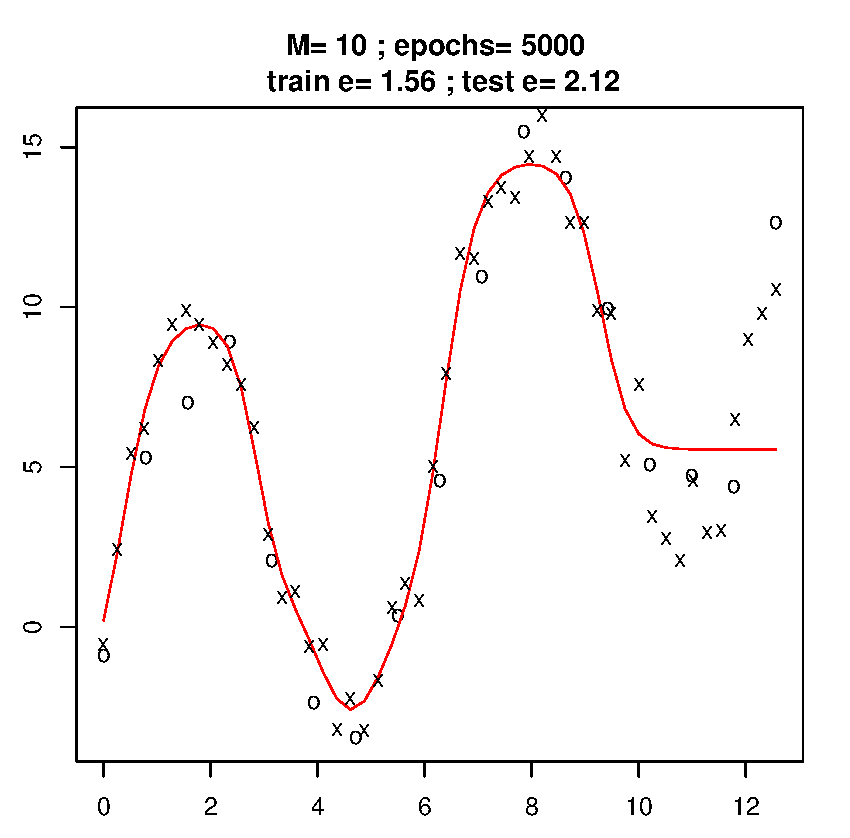
\includegraphics[width=60mm]{03Ann/annapp/simpleM10E5000.eps}&    
%		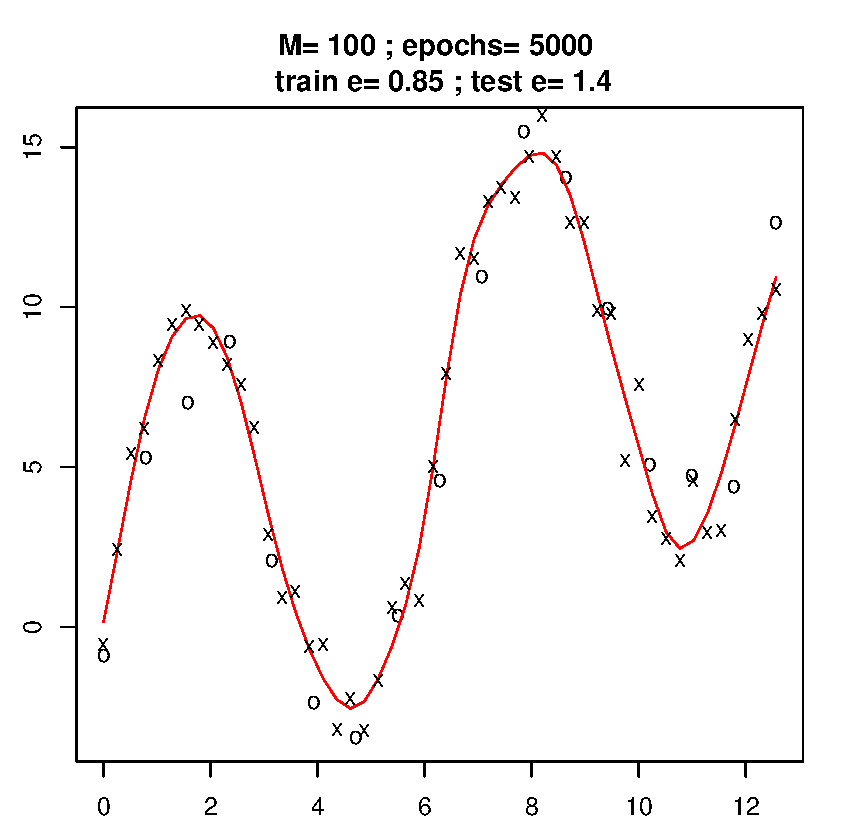
\includegraphics[width=60mm]{03Ann/annapp/simpleM100E5000.eps}     \\
%		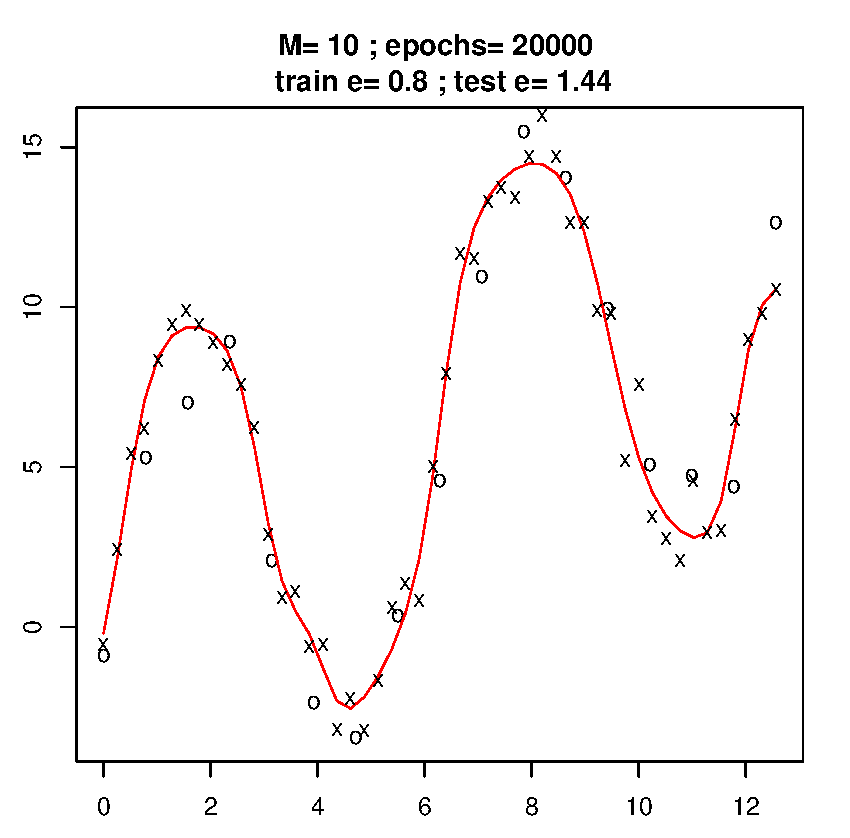
\includegraphics[width=60mm]{03Ann/annapp/simpleM10E20000.eps}    &    
%		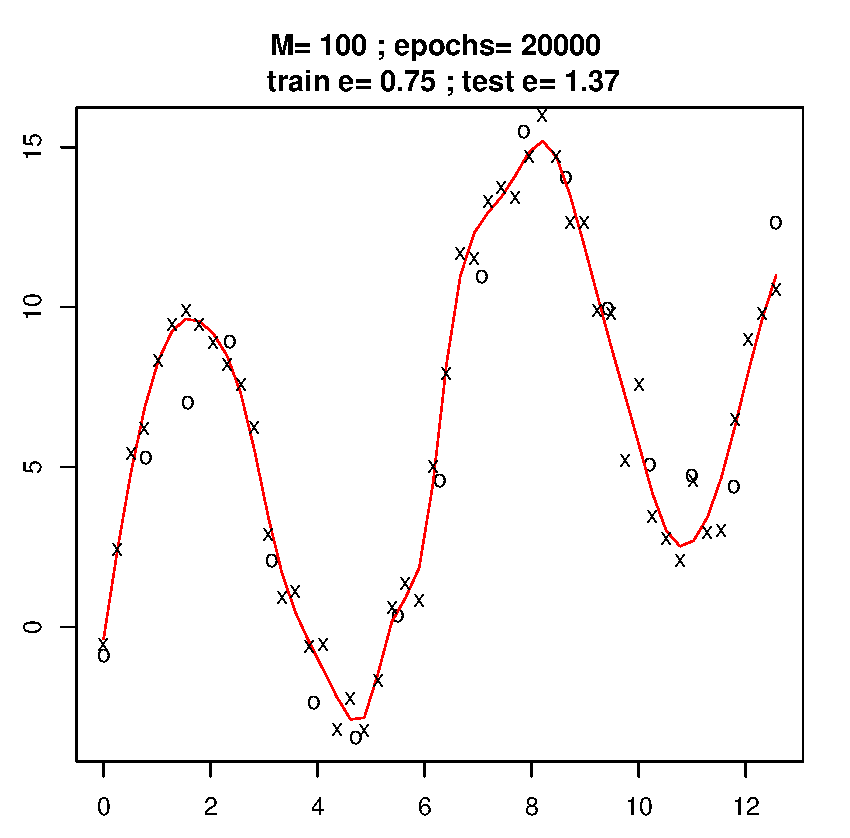
\includegraphics[width=60mm]{03Ann/annapp/simpleM100E20000.eps}     \\
%		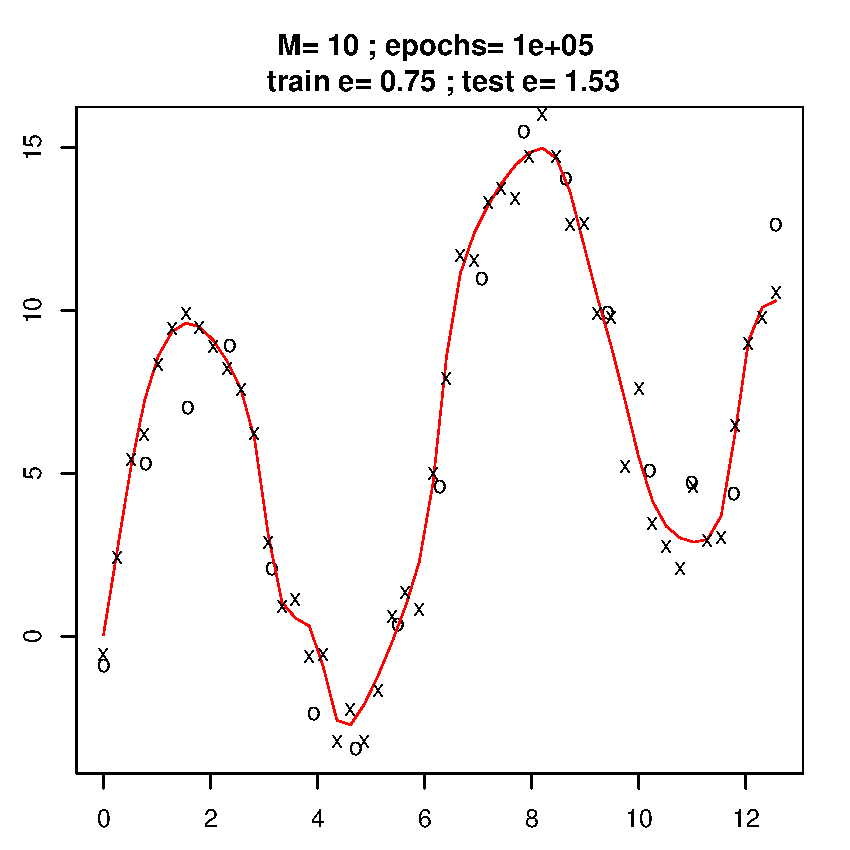
\includegraphics[width=60mm]{03Ann/annapp/simpleM10E100000.eps}&    
%		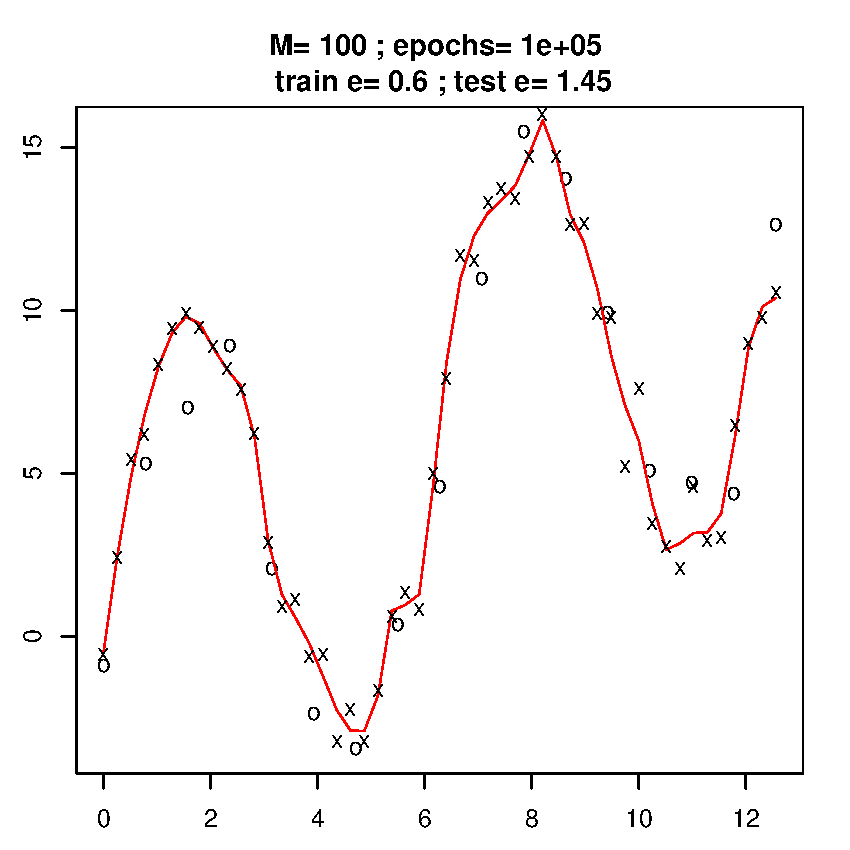
\includegraphics[width=60mm]{03Ann/annapp/simpleM100E100000.eps}           
%	\end{tabular}
%\end{figure}




\section{คำแนะนำสำหรับการใช้แบบจำลองทำนาย}
\label{sec: practical suggestions}

การประเมินผล เป็นกลไกที่สำคัญมากสำหรับการใช้แบบจำลองทำนาย.
แต่หากผลที่ประเมินได้ไม่น่าพอใจ และต้องการปรับปรุงให้ได้ผลการทำนายดีขึ้น
มีทางเลือกต่าง ๆ มากมาย เช่น
การเพิ่มจำนวนข้อมูลที่จะใช้สำหรับการฝึก %(collect more training examples)
หรือการคัดเลือกตัวแปรต้นของข้อมูล โดยเลือกเฉพาะ\textit{คุณลักษณะ}ที่สำคัญ  นั่นคือเลือกเฉพาะมิติ บางมิติที่สำคัญ มาใช้เป็นอินพุตสำหรับแบบจำลอง %ลักษณะที่สำคัญมาเป็นอินพุต (select smaller sets of features)
หรือการเพิ่ม\textit{คุณลักษณะ}ใหม่เข้าไปในอินพุตของแบบจำลอง %(get additional features)
หรือการเพิ่ม\textit{ความซับซ้อน}ของแบบจำลองขึ้น %(try increase model's complexity)
หรือการลด\textit{ความซับซ้อน}ของแบบจำลองลง. %(try decrease model's complexity)

ทางเลือกที่หลากหลาย อาจทำให้สับสนได้
และการปรับปรุงแบบจำลอง
ควรจะลองทำอะไรก่อน อะไรหลัง
ซึ่งการลองทำแต่ละอย่าง อาจใช้เวลามาก และยังอาจเพิ่มงบประมาณด้วย 
เช่น การออกไปหาข้อมูลมาเพิ่ม (เพิ่มจำนวนจุดข้อมูล) 
หรือการเพิ่มลักษณะสำคัญชนิดใหม่เข้าไป (เพิ่มมิติใหม่สำหรับอินพุต).
ผู้เชี่ยวชาญศาสตร์การเรียนรู้ของเครื่อง
แอนดรูว์ อึ้ง\cite{Ng2013a} แนะนำว่า
ก่อนตัดสินใจเลือกทดลองปรับปรุงด้วยวิธีใด
ควรทำการทดลองง่าย ๆ 
และใช้\textbf{เส้นโค้งเรียนรู้} (Learning Curve) เป็นตัวชี้แนะ.
\index{english}{learning curve}
\index{thai}{เส้นโค้งเรียนรู้}
การใช้\textit{เส้นโค้งเรียนรู้}
มีพื้นฐานมาจากการศึกษาเรื่องคุณภาพการทำนาย
ที่สัมพันธ์กับ\textit{ความลำเอียง} (bias%
\footnote{ในบริบทของพฤติกรรมโดยรวมของแบบจำลอง ไม่ใช่บริบทของพารามิเตอร์ของโครงข่ายประสาทเทียม.})
\index{english}{bias (model behavior)}
\index{thai}{ความลำเอียง}
และ\textit{ความแปรปรวน} (variance).
\index{english}{variance (model behavior)}
\index{thai}{ความแปรปรวน}

\subsection{ความลำเอียงกับความแปรปรวน}
\label{sec: bias v.s. variance}
\index{english}{bias-variance}
\index{thai}{ความลำเอียงกับความแปรปรวน}



พิจารณารูป~\ref{fig: multiple degs polynomial fitting}
ที่ใช้\textit{ฟังก์ชันพหุนาม}ทำนายข้อมูล.
ภาพ ข ใน รูป~~\ref{fig: train and test data}
แสดงค่าผิดพลาดที่ได้ต่อระดับขั้น. 
ระดับขั้น บอกความซับซ้อนของแบบจำลองฟังก์ชันพหุนาม.
ที่ความซับซ้อนของแบบจำลองที่เหมาะสม ค่าผิดพลาดของชุดข้อมูลทดสอบ
จะมีค่าต่ำที่สุด.

ฟังก์ชันพหุนามระดับขั้นเก้าก็\textit{โอเวอร์ฟิต}ข้อมูลอย่างชัดเจน.
ส่วนฟังก์ชันพหุนามระดับขั้นศูนย์ ระดับขั้นหนึ่ง และระดับขั้นสอง\textit{อันเดอร์ฟิต}ของข้อมูลอย่างชัดเจน.
การ\textbf{อันเดอร์ฟิต} (underfit)
หมายถึง
การที่ความซับซ้อนของแบบจำลอง
ไม่เพียงพอที่จะประมาณความสัมพันธ์ของข้อมูลได้.
\index{english}{underfit}
\index{thai}{อันเดอร์ฟิต}
%
ช่วงที่ความซับซ้อนของแบบจำลองน้อยเกินไป %ซึ่งคือกรณีการ\textit{อันเดอร์ฟิต}
มีจุดสังเกตสำคัญคือ ค่าผิดพลาดจะสูงกับทั้งข้อมูลชุดทดสอบและชุดฝึกหัด.
เมื่อความซับซ้อนของแบบจำลองไม่พอ
แบบจำลองจะไม่ยืดหยุ่นพอที่ปรับตัว
เพื่อลดค่าผิดพลาดกับข้อมูลชุดฝึกลงได้.
กรณีที่แบบจำลองทำงานได้ไม่ดี
เนื่องจาก\textit{ความซับซ้อนของแบบจำลองน้อยเกินไป}นี้ จะเรียกว่า กรณีที่มี\textit{ความลำเอียงสูง} (high bias) 
ซึ่งสื่อถึงการ\textit{อันเดอร์ฟิต}.
\index{english}{high bias}
\index{thai}{ความลำเอียงสูง}

ส่วนกรณีที่ความซับซ้อนของแบบจำลองมากเกินไป
ซึ่งคือกรณีการ\textit{โอเวอร์ฟิต}มีจุดสังเกตที่สำคัญคือ ค่าผิดพลาดกับชุดฝึกจะต่ำมาก แต่ค่าผิดพลาดกับชุดทดสอบจะสูง.
%ความต่างระหว่างค่าผิดพลาดของชุดฝึกหัดกับชุดทดสอบมีค่ามาก.
แบบจำลองที่มีความซับซ้อนมาก
จะสามารถปรับพฤติกรรมการทำนาย
เพื่อลดค่าผิดพลาดกับข้อมูลชุดฝึกหัดลงได้ดี
แต่หากความซับซ้อนมากเกินไป จนไปลดค่าผิดพลาดกับข้อมูลชุดฝึกหัดที่เกิดจากสัญญาณรบกวนด้วย แบบจำลองจะทำนายข้อมูลชุดทดสอบได้ไม่ดี.
กรณีนี้จะเรียกว่า เป็นกรณีที่มี\textit{ความแปรปรวนสูง} (high variance) 
ซึ่งสื่อถึงการ\textit{โอเวอร์ฟิต}.
\index{english}{high variance}
\index{thai}{ความแปรปรวนสูง}

กล่าวอีกอย่างหนึ่ง \textit{ความลำเอียงสูง}
หมายถึงแบบจำลองของไม่ยืดหยุ่นมากพอ 
ส่วน\textit{ความแปรปรวนสูง}หมายถึงแบบจำลองของยืดหยุ่นมากเกินไป.
%
แบบจำลองที่ดีที่สุดที่ทำได้ คือ แบบจำลองที่ลดให้ทั้ง\textit{ความลำเอียง}และ\textit{ความแปรปรวน}มีค่าต่ำ.
แต่ไม่ว่าแบบจำลองไหนก็ตาม เราทำดีที่สุด ได้แค่ดีที่สุด จะฝืนข้อจำกัดของธรรมชาติไม่ได้.

ทฤษฎีที่กล่าวถึงข้อจำกัดของการทำแบบจำลองนี้คือ \textbf{ทวิบถของความลำเอียงกับความแปรปรวน} (ฺBias/Variance Dilemma).
\index{english}{Bias/Variance Dilemma}
\index{thai}{ทวิบถของความลำเอียงกับความแปรปรวน}
\textit{ทวิบถของความลำเอียงกับความแปรปรวน} 
เสนอโดย
เจมันและคณะ\cite{GemanEtAl1992a} จากการศึกษาความสามารถ
และขีดจำกัดของการทำแบบจำลอง.
\textit{ทวิบถของความลำเอียงกับความแปรปรวน}
สรุปว่า เราสามารถทำแบบจำลองให้ดีที่สุดได้
โดยลดทั้งค่าความลำเอียงและความแปรปรวนให้ต่ำ.
แต่ค่าผิดพลาดก็มีขีดจำกัดหนึ่ง (ขึ้นกับธรรมชาติของปัญหา) ที่เราไม่สามารถลดค่าผิดพลาดลงไปให้ต่ำกว่านั้นได้. การที่เราพยายามจะลดค่าผิดพลาดให้ต่ำกว่านั้น
โดยการลดส่วนหนึ่ง ก็จะไปเพิ่มอีกส่วน 
เช่น หากพยายามลดค่าผิดพลาดจากความลำเอียงมากเกินไป ก็จะทำให้ส่วนที่เกิดจากความแปรปรวนเพิ่ม 
และในทางกลับกัน
หากพยายามลดค่าผิดพลาดจากความแปรปรวนมากเกินไป ก็จะทำให้ส่วนที่เกิดจากความลำเอียงเพิ่ม. 

\subsection{เส้นโค้งเรียนรู้}
\label{sec: learning curve}
\index{english}{Learning Curve} \index{thai}{เส้นโค้งเรียนรู้}
\textbf{เส้นโค้งเรียนรู้} (Learning Curve)
เป็นเครื่องมือช่วยแสดงความสัมพันธ์ระหว่างความพยายามที่ใช้ไปในการฝึกแบบจำลอง
กับผลการทำงานของแบบจำลอง.
\textit{เส้นโค้งเรียนรู้}
สามารถใช้เพื่อช่วยให้เงื่อนงำว่า แบบจำลองที่ใช้อยู่
มีความเสี่ยงที่จะมี\textit{ความลำเอียง}สูง
หรือเสี่ยงที่จะมี\textit{ความแปรปรวน}สูง.
เส้นโค้งเรียนรู้ สร้างโดย การตรวจสอบ\textit{ผลการฝึกแบบจำลอง}ที่จำนวนจุดข้อมูลฝึกต่าง ๆ 
แล้วนำค่าผิดพลาดเฉลี่ยกับชุดฝึก
และค่าผิดพลาดเฉลี่ยกับชุดทดสอบ
มาวาดกราฟ ดังแสดงในรูป~\ref{fig: learning curve high bias vs high variance}.

การวัดค่าผิดพลาดกับชุดฝึก
วัดเฉพาะกับจุดข้อมูลที่ใช้ฝึก
เช่น หากฝึกแบบจำลองด้วย $10$ จุดข้อมูล ก็หาค่าผิดพลาดของการทำนายค่า $10$ จุดข้อมูลนี้.
ดังนั้น เมื่อจำนวนจุดข้อมูลฝึกน้อย
แบบจำลองมีโจทย์ที่ต้องทำน้อย
ก็มีโอกาสที่จะทำค่าผิดพลาดของชุดฝึกน้อยด้วย.
เมื่อเพิ่มจำนวนจุดข้อมูลฝึกขึ้น ค่าผิดพลาดของชุดฝึกก็จะเพิ่มขึ้น
และลู่เข้าสู่ค่า ๆ หนึ่ง.
ในขณะเดียวกัน เมื่อจำนวนจุดข้อมูลฝึกเพิ่มขึ้น ค่าผิดพลาดของชุดทดสอบจะลดลงจนลู่เข้าสู่ค่า ๆ หนึ่ง.

ในกรณีที่ แบบจำลองมีความเสี่ยงจาก\textit{ความลำเอียง}สูง
ถ้าข้อมูลทดสอบ และข้อมูลฝึกมีปริมาณเพียงพอ
พฤติกรรมการทำนายของแบบจำลอง
จะให้ผลในลักษณะเดียวกัน
และทำให้ค่าผิดพลาดจากชุดฝึก
และจากชุดทดสอบ
มีค่าใกล้เคียงกัน.
แต่กรณีที่แบบจำลองมี\textit{ความแปรปรวน}สูง นั่นคือ แบบจำลองมีความยืดหยุ่นมากเกินไป มากจนพอที่จะปรับตัวเข้ากับสัญญาณรบกวนในข้อมูลฝึกได้.
ผลคือแบบจำลองสามารถลดค่าผิดพลาดของชุดฝึกได้ต่ำ
และทำให้ผลต่างระหว่างค่าผิดพลาดจากชุดฝึก
และจากชุดทดสอบมีค่าต่างกัน.
ดังนั้นความต่างระหว่างค่าผิดพลาดจากข้อมูลทดสอบและจากข้อมูลฝึกจึงสามารถใช้บ่งชี้สถานการณ์คร่าว ๆ ของแบบจำลองได้.

%
\begin{figure}
	\begin{center}
\begin{tabular}{cc}
\includegraphics[width=0.4\columnwidth]{03Ann/annapp/highbias.png}
&
\includegraphics[width=0.4\columnwidth]{03Ann/annapp/highvariance.png}		
\end{tabular} 		
\end{center}
	\caption[เส้นโค้งเรียนรู้]{ภาพวาด\textit{เส้นโค้งเรียนรู้}.
	 ภาพซ้าย แสดงกรณีแบบจำลองมีความลำเอียงสูง. 
เมื่อจำนวนจุดข้อมูลฝึกมากขึ้น ค่าผิดพลาดกับชุดฝึก
และค่าผิดพลาดกับชุดทดสอบ
มีค่าใกล้เคียงกัน.
ภาพขวา แสดงกรณีแบบจำลองมีความแปรปรวนสูง. เมื่อจำนวนของจุดข้อมูลฝึกมากขึ้น ค่าผิดพลาดกับชุดฝึก
และค่าผิดพลาดกับชุดทดสอบ
มีค่าต่างกัน.}
	\label{fig: learning curve high bias vs high variance}
\end{figure}

รูป~\ref{fig: learning curve high bias vs high variance} เป็นภาพวาดเพื่อให้เห็นภาพรวม
แต่
ในสถานการณ์จริง \textit{เส้นโค้งเรียนรู้}ที่ได้
อาจจะมีสัญญาณรบกวนมาก 
หรือแม้แต่สเกลของการวาดกราฟ
อาจทำให้ต้องใช้ความระมัดระวัง
ในการอ่านผลจากเส้นโค้งเรียนรู้.
%
รูป~\ref{fig: learning-curve tests}
แสดงกระบวนการทดสอบแบบจำลอง เพื่อวาด\textit{เส้นโค้งเรียนรู้}.
%(แบบฝึกหัด~\ref{ex: learning curve})
รูป~\ref{fig: real learning curves} แสดงเส้นโค้งเรียนรู้ที่ได้จาก
%ตัวอย่างการทดลองขนาดเล็ก.
%หมายเหตุ ตัวอย่างนี้เลือกสถานการณ์เพื่อให้เห็นภาพได้ชัดเจน.
%และดำเนินการทดลองโดยใช้ทรัพยากรไม่มากเกินไป.
%รูป~\ref{fig: learning-curve tests}
%และ~\ref{fig: real learning curves}
%แสดง
แบบจำลองที่มีความซับซ้อนต่าง ๆ กัน
เพื่อให้เห็นตัวอย่างลักษณะของเส้นโค้งเรียนรู้
ในกรณีต่าง ๆ.
%การใช้เส้นโค้งเรียนรู้
%ก็เพื่อที่จะเป็นตัวบ่งชี้
%และลดความจำเป็นที่จะต้องทดลองกับหลาย ๆ แบบจำลองแทนการทดลองที่จะใช้ทรัพยากรเช่นนี้.
%
%ในสถานการณ์จริง อาจทดลองหลาย ๆ แบบจำลองในลักษณะนี้ได้ยาก เนื่องจากทรัพยากรที่ต้องการ เช่น เวลาและแรงงานในการฝึกและทดสอบแต่ละแบบจำลอง โดยเฉพาะแบบจำลองที่มีความซับซ้อนสูงอาจต้องการเวลาและแรงงานในการฝึกมาก.
%การใช้\textit{เส้นโค้งเรียนรู้} ก็เพื่อที่จะเป็นแนวทางว่าแบบจำลองใหม่ที่จะสร้างมาเปรียบเทียบเช่นนี้
%ควรจะเลือก
%
%ใช้ทดสอบแบบจำลองเดียวที่มีอยู่ สำหรับตัดสินใจว่าควรจะปรับปรุงแบบจำลองนี้อย่างไร ก่อนที่จะลองสร้างแบบจำลองใหม่ขึ้นมา

จากรูป~\ref{fig: learning-curve tests} และคำบรรยาย
แบบจำลองโครงข่ายประสาทเทียมสองชั้น
ขนาด $4$ หน่วยซ่อน \textit{อันเดอร์ฟิต}ข้อมูล
และ\textit{เส้นโค้งเรียนรู้} ก็ลู่เข้าหากัน
โดยอัตราความต่างระหว่างค่าผิดพลาดจากชุดทดสอบและชุดฝึกค่อนข้างต่ำ (ประมาณ $1.55$).
แบบจำลองโครงข่ายประสาทเทียมสองชั้นขนาด $200$ หน่วยซ่อน \textit{โอเวอร์ฟิต}ข้อมูลอย่างชัดเจน (รูป~\ref{fig: learning-curve tests})
และ\textit{เส้นโค้งเรียนรู้}ก็ลู่เข้าห่างกันชัดเจน
โดยอัตราความต่างระหว่างค่าผิดพลาดจากชุดทดสอบและชุดฝึกสูง (ประมาณ $5.62$ รูป~\ref{fig: real learning curves}).



%
\begin{figure} %[H]
	\begin{center}
		\begin{tabular}{c}
\includegraphics[width=\columnwidth]
			{03Ann/annapp/predictM4.png}
\\
\includegraphics[width=\columnwidth]
{03Ann/annapp/predictM16.png}
\\
\includegraphics[width=\columnwidth]
{03Ann/annapp/predictM64.png}
\\
\includegraphics[width=\columnwidth]
{03Ann/annapp/predictM100.png}
\\
\includegraphics[width=\columnwidth]
			{03Ann/annapp/predictM200.png}
		\end{tabular} 			
	\end{center}
\caption[ตัวอย่างพฤติกรรมของแบบจำลองที่ความซับซ้อนต่าง ๆ]{ตัวอย่างกระบวนการทดสอบแบบจำลองเพื่อวาด\textit{เส้นโค้งเรียนรู้}
สำหรับโครงข่ายประสาทเทียมสองชั้น ขนาด $4$ ขนาด $16$ ขนาด $64$ ขนาด $100$ และขนาด $200$ หน่วยซ่อน จากแถวบนลงล่าง ตามลำดับ. 
แต่ละแถวแสดง $5$ ภาพ ที่แต่ละภาพเป็นการฝึกกับข้อมูลฝึกขนาด $8$ จุด
ขนาด $16$ จุด ขนาด $24$ จุด ขนาด $32$ จุด และขนาด $40$ จุด จากซ้ายมาขวา ตามลำดับ. 
แต่ละภาพใช้กากบาทสีฟ้าแสดงจุดข้อมูลฝึก และใช้วงกลมสีแดงแสดงจุดข้อมูลทดสอบ
เส้นสีเขียวแสดงค่าที่แบบจำลองที่ฝึกเสร็จแล้วทำนาย.
ชื่อแต่ละภาพระบุความซับซ้อนของแบบจำลองด้วยจำนวนหน่วยซ่อน และระบุจำนวนจุดข้อมูลที่ใช้ฝึก.
ตัวอย่างนี้ เพื่อแสดงในเห็นกระบวนการดำเนินการอย่างชัดเจน และเพื่อเปรียบเทียบผลของเส้นโค้งเรียนรู้.
ในสถานการณ์จริง การใช้เส้นโค้งเรียนรู้ ก็เพื่อหลีกเลี่ยงการที่จะต้องทดลองโดยตรงกับหลาย ๆ แบบจำลองเช่นนี้.
\textit{ค่ารากสองของค่าเฉลี่ยค่าผิดพลาดกำลังสอง}ของโครงข่ายสองชั้นกับ\textit{ข้อมูลทดสอบ} 
$40$ จุด
คือ
$1.48$,
$1.14$,
$1.40$,
$1.39$,
และ $1.58$ เมื่อใช้หน่วยซ่อน
$4$, $16$, $64$, $100$, 
และ $200$ หน่วยตามลำดับ.
}
	\label{fig: learning-curve tests}
\end{figure}

%4 = RMSE =  1.48064555297
%16 = RMSE =  1.13918654497
%64 = RMSE =  1.39957246803
%100 = RMSE =  1.38691844958
%200 = RMSE =  1.58293197337




%
\begin{figure} %[H]
	\begin{center}
\begin{tabular}{ccc}
\includegraphics[width=0.3\columnwidth]
{03Ann/annapp/learncurvM4.png}
&
\includegraphics[width=0.3\columnwidth]
{03Ann/annapp/learncurvM16.png}	
&
\includegraphics[width=0.3\columnwidth]
{03Ann/annapp/learncurvM64.png}
\\	
\includegraphics[width=0.3\columnwidth]
{03Ann/annapp/learncurvM100.png}	
&
\includegraphics[width=0.3\columnwidth]
{03Ann/annapp/learncurvM200.png}
&
\includegraphics[width=0.3\columnwidth]
{03Ann/annapp/gaps.png}
\end{tabular} 			
	\end{center}
	\caption[ตัวอย่างเส้นโค้งเรียนรู้]{ตัวอย่างเส้นโค้งเรียนรู้ จากแบบจำลองขนาด $4$, $16$, $64$, $100$, และ $200$ หน่วยซ่อน ตามที่ระบุในชื่อแต่ละภาพ. ภาพล่างขวา แสดงความต่างระหว่างค่าผิดพลาดจากข้อมูลฝึกกับค่าผิดพลาดจากข้อมูลทดสอบ (แกนตั้ง) และความซับซ้อนของแบบจำลอง (แกนนอน). 
	ความต่างแสดงในรูปแบบอัตราส่วน
	นั่นคือ  $E_{\mathrm{test}}/E_{\mathrm{train}}$
เมื่อ $E_{\mathrm{test}}$ คือรากที่สองของค่าเฉลี่ยค่าผิดพลาดกำลังสอง
จากข้อมูลทดสอบ และ $E_{\mathrm{train}}$ คือ จากข้อมูลฝึก.
ความต่างในภาพ คือ
$1.55$, $1.77$, $2.97$, $2.77$, และ $5.62$ สำหรับแบบจำลองขนาด $4$, $16$, $64$, $100$, และ $200$ หน่วยซ่อน ตามลำดับ.
}
\label{fig: real learning curves}
\end{figure}
%

หลังจากพอรู้แล้วว่า 
สถานการณ์อยู่ในกรณี\textit{ความลำเอียง}
หรืออยู่ในกรณี\textit{ความแปรปรวน}สูง
แอนดรูว์ อึ้ง\cite{Ng2013a}
แนะนำให้พิจารณาทางเลือก ดังนี้
\begin{itemize}
	\item \emph{เก็บข้อมูลมาเพิ่มสำหรับการฝึก.} % (collect more training examples),
	การเพิ่มจำนวนข้อมูลในการฝึก จะช่วยในกรณี\textit{ความแปรปรวน}สูง.
	\item \emph{เลือกเฉพาะบางมิติของข้อมูลมาเป็นอินพุต.} % (select smaller sets of features),
	การเลือกเฉพาะบางมิติของข้อมูลมาเป็นอินพุต. 
	การลดมิติของอินพุตลง
	ก็จะช่วยในกรณี\textit{ความแปรปรวน}สูง
	โดยเฉพาะ
สำหรับโครงข่ายประสาทเทียม.
ตัวอย่าง เช่น โครงข่ายประสาทเทียมสองชั้น
ที่มีจำนวนหน่วยซ่อนเท่าเดิม
การลดมิติของอินพุตลง เท่ากับลดจำนวนพารามิเตอร์ลง.
	\item \emph{เพิ่มลักษณะที่สำคัญใหม่เข้าไปในอินพุต.} % (get additional features),
	การเพิ่มลักษณะที่สำคัญใหม่เข้าไปในอินพุต การเพิ่มมิติของอินพุตขึ้น โดยทั่วไปแล้ว จะช่วยในกรณี\textit{ความลำเอียง}สูง.
	\item \emph{เพิ่มความซับซ้อนของแบบจำลองขึ้น.} % (try increase model's complexity), 
	การเพิ่มความซับซ้อนของแบบจำลอง เช่น การเพิ่มจำนวนหน่วยซ่อน จะช่วยในกรณี\textit{ความลำเอียง}สูง.
	\item \emph{ลดความซับซ้อนของแบบจำลองลง.} % (try decrease model's complexity),
	การลดความซับซ้อนของแบบจำลอง เช่น การลดจำนวนหน่วยซ่อน การทำ\textit{เรกูลาไรซ์} หรือ การทำ\textit{การหยุดก่อนกำหนด} จะช่วยในกรณี\textit{ความแปรปรวน}สูง.
\end{itemize}

ตาราง~\ref{tbl: ann tips options by bias variance} 
สรุปทางเลือกที่แอนดรูว์ อึ้ง\cite{Ng2013a}
แนะนำ
สำหรับกรณีความลำเอียงสูง
และกรณีความแปรปรวนสูง.
สุดท้าย
หากลองวิธีทั่ว ๆ ไปดังนี้แล้ว ผลยังไม่น่าพอใจ
อาจจะลองวิเคราะห์ และตรวจสอบผลที่\textit{ขั้นตอนวิธี}ทำผิด ดูว่าผิดลักษณะไหน อย่างไร.
เผื่อว่า อาจจะพบคุณสมบัติเฉพาะบางอย่างที่ผลมักจะผิด เช่น 
หากเป็นการจำแนกตัวเลขจากภาพ \textit{ขั้นตอนวิธี}ที่ใช้ อาจจะจำแนกเลข 2 เป็นเลข 4 บ่อย ๆ ซึ่งเมื่อดูภาพของเลขที่จำแนกผิด ก็อาจพบว่า มีรูปแบบการเขียนเลข 2 แบบหนึ่ง ที่มักจะจำแนกผิด.
หากพบรูปแบบเฉพาะนั้น อาจเพิ่มการจัดการพิเศษเฉพาะสำหรับรูปแบบนั้นได้.

%* Start w/ a simple algorithm that you can implement quickly (1 day). Implement it and test it on your cross validation data.
%* Plot learning curves to decide if more data, more featue, etc. are likely to help.
%* Do error analysis: manually examine the examples that your algorithm made errors on. See if you spot any systematic trend in what type of examples it is makig errors on.

\begin{table}[hbtp]
%	{\footnotesize %scriptsize
		\caption[สรุปคำแนะนำสำหรับปรับปรุงแบบจำลอง]{สรุปทางเลือกที่แนะนำในกรณีความลำเอียงสูงและความแปรปรวนสูง.}
		\label{tbl: ann tips options by bias variance}
		\begin{center}
			\begin{tabular}{|l|c|c|}
				\hline 
				& \multicolumn{2}{c|}{กรณี} \\
				\cline{2-3}
				ทางเลือก & ความลำเอียงสูง & ความแปรปรวนสูง \\
				\hline
				เพิ่มรอบฝึก            & แนะนำ      &   \\
				เพิ่มจำนวนหน่วยย่อย     & แนะนำ      &   \\
				ทำเรกูลาไรซ์        &           & แนะนำ \\
				ทำหยุดก่อนกำหนด    &           & แนะนำ \\
				ลดมิติของอินพุตลง       &           & แนะนำ \\
				เพิ่มมิติของอินพุตขึ้น      & แนะนำ      &  \\
				เพิ่มจำนวนจุดข้อมูลฝึก     &             & แนะนำ \\
				%
				\hline
			\end{tabular} 
		\end{center}
%	}%end \small
\end{table}




% LATER
%\section{แผนที่การจัดระเบียบตัวเอง}
%\label{sec: SOM}


%\section{Glossary}
\section{อภิธานศัพท์}

\begin{description}
	
	\item[การปรับเส้นโค้ง (curve fitting):] 
\index{thai}{การปรับเส้นโค้ง}
\index{english}{curve fitting}	
การปรับพฤติกรรมของแบบจำลองทำนาย 
โดยการเปลี่ยนค่าของพารามิเตอร์ เพื่อให้พฤติกรรมทำนายสอดคล้องกับข้อมูลที่มี.

\item[จุดข้อมูล (datapoint):] 
\index{thai}{จุดข้อมูล}
\index{english}{datapoint}	
ตัวอย่างข้อมูลที่มีค่าของตัวแปรต้น $x$ และตัวแปรตาม $y$ ที่เป็นคู่กัน.

\item[ฟังก์ชันพหุนาม (polynomial function):] 
\index{thai}{ฟังก์ชันพหุนาม}
\index{english}{polynomial function}	
ฟังก์ชัน $f: \mathbb{R} \mapsto \mathbb{R}$
ที่แสดงความสัมพันธ์ระหว่างตัวแปรต้น $x$ และตัวแปรตาม $y$ ด้วยสมการพหุนาม
$y = f(x, \bm{w}) = \sum_{m=0}^M w_m x^m$
เมื่อ พารามิเตอร์ของฟังก์ชัน $\bm{w}$ $= [w_0, \; w_1, \; \ldots, \; w_M]^T$.

\item[การฝึก (training):] 
\index{thai}{การฝึก}
\index{english}{training}	
\index{thai}{การเรียนรู้}
\index{english}{learning}
การฝึก หรือการเรียนรู้ คือการปรับค่าพารามิเตอร์ของแบบจำลอง เพื่อให้แบบจำลองมีพฤติกรรมการทำนายสอดคล้องกับข้อมูล.

\item[ค่าเฉลย (ground truth):] 
\index{thai}{ค่าเฉลย}
\index{english}{ground truth}	
ค่าของตัวแปรตาม $y$ จากข้อมูล ที่คู่กับตัวแปรต้น $x$ ที่สนใจ.

\item[คุณสมบัติความทั่วไป (generalization):] 
\index{thai}{คุณสมบัติความทั่วไป}
\index{english}{generalization}	
ความสามารถของแบบจำลองทำนาย ที่สามารถทำนายข้อมูลที่ไม่เคยเห็นได้ดี.

\item[ข้อมูลฝึก (training data):] 
\index{thai}{ข้อมูลฝึก}
\index{english}{training data}	
ข้อมูลที่ใช้ในกระบวนการฝึกแบบจำลอง

\item[ข้อมูลทดสอบ (test data):] 
\index{thai}{ข้อมูลทดสอบ}
\index{english}{test data}	
ข้อมูลที่ใช้ในทดสอบแบบจำลอง.

\item[การโอเวอร์ฟิต (overfitting):] 
\index{thai}{โอเวอร์ฟิต}
\index{english}{overfitting}	
การที่แบบจำลองสามารถทำนายข้อมูลฝึกได้ดี แต่ทำนายข้อมูลใหม่ที่ไม่เคยเห็นได้ไม่ดี
นั่นคือ การที่แบบจำลองไม่มีคุณสมบัติความทั่วไป.

\item[ความซับซ้อนของแบบจำลอง (model complexity):] 
\index{thai}{ความซับซ้อนของแบบจำลอง}
\index{english}{model complexity}	
การยืดหยุ่นของแบบจำลอง อาจบ่งชี้ได้จากจำนวนพารามิเตอร์ของแบบจำลอง.

\item[โครงข่ายประสาทเทียม (artificial neural network):]
แบบจำลองคำนวณ
ที่ทำการคำนวณ
โดยใช้หน่วยคำนวณย่อยหลาย ๆ หน่วย
ที่แต่ละหน่วยทำการคำนวณในแบบคล้าย ๆ กัน.

\item[เพอร์เซปตรอนหลายชั้น (multi-layer perceptron):]
โครงข่ายประสาทเทียม
ที่หน่วยคำนวณต่าง ๆ ต่อกันเป็นโครงข่ายในลักษณะชั้นคำนวณ.

\item[โหนด หรือหน่วยคำนวณ (node หรือ unit):]
การคำนวณย่อยของโครงข่ายประสาทเทียม
ที่มีลักษณะการคำนวณง่าย ๆ ไม่ซับซ้อน.

\item[ชั้นคำนวณ (layer):]
กลุ่มของโหนด ในโครงข่ายประสาทเทียม
ที่จัดโครงสร้างเป็นลักษณะชั้นคำนวณ
โดย
กลุ่มของโหนดในชั้นคำนวณเดียวกัน
จะรับอินพุตจาก(กลุ่มของโหนดใน)ชั้นคำนวณก่อนหน้า
หรือจะส่งเอาต์พุตออกไปให้(กลุ่มของโหนดใน)ชั้นคำนวณถัดไป
หรือทั้งสองอย่าง.

\item[ชั้นซ่อน (hidden layer):]
ชั้นคำนวณที่จะส่งเอาต์พุตออกไปให้(กลุ่มของโหนดใน)ชั้นคำนวณถัดไป
โดยเอาต์พุตของชั้นซ่อนจะไม่ใช่เอาต์พุตสุดท้ายของโครงข่าย.

\item[หน่วยซ่อน (hidden node หรือ hidden unit):]
โหนดในชั้นซ่อน.

\item[ค่าน้ำหนักและค่าไบอัส (weights and biases):]
ค่าพารามิเตอร์ต่าง ๆ ของโครงข่ายประสาทเทียม.

\item[ฟังก์ชันกระตุ้น (activation function):]
ฟังก์ชันคำนวณของโหนด.

\item[ชั้นเอาต์พุต (output layer):]
ชั้นคำนวณชั้นสุดท้าย
ที่เอาต์พุตของชั้น จะเป็นเอาต์พุตของโครงข่าย.

\item[การแพร่กระจายย้อนกลับ (backpropagation หรือ error backpropagation):]
ขั้นตอนวิธีการคำนวณหาค่าเกรเดียนต์ เพื่อปรับค่าน้ำหนัก สำหรับโครงข่ายประสาทเทียม.

\item[การฝึกแบบหมู่ (batch training):]
การฝึกที่ใช้ข้อมูลฝึกทั้งหมดทีเดียว
นั่นคือ การปรับค่าพารามิเตอร์ทำเดียวในแต่ละสมัยฝึก.

\item[การฝึกแบบออนไลน์ (online training):]
การฝึกที่ใช้ข้อมูลฝึกทีละหนึ่งจุดข้อมูล
นั่นคือ การปรับค่าพารามิเตอร์จะทำหลาย ๆ ครั้ง
แต่ละครั้งสำหรับแต่ละจุดข้อมูล
และจะทำจนกว่าจะครบทุกจุดข้อมูล ในแต่ละสมัยฝึก.

\item[สมัย (epoch):]
รอบการปรับค่าพารามิเตอร์
โดยแต่ละรอบจะนับเมื่อมีการใช้ข้อมูลฝึกครบทุกจุด.

\item[อัตราเรียนรู้ (learning rate):]
ขนาดก้าว ที่เป็นค่าสเกล่าร์
เพื่อควบคุมความเร็วในการฝึกแบบจำลอง
เป็นค่าที่ใช้กับ\textit{ขั้นตอนวิธีการหาค่าดีที่สุด}ที่อยู่เบื้องหลังการฝึก.

\item[การกำหนดค่าน้ำหนักเริ่มต้น (weight initialization):]
การกำหนดค่าน้ำหนักและไบอัส
ให้กับโครงข่ายประสาทเทียม ก่อนการฝึก.

\item[การจำแนกค่าทวิภาค (binary classification):]
ภาระกิจการทำนาย ที่ผลการทำนายมีได้สองแบบ.

\item[ฟังก์ชันสูญเสียครอสเอนโทรปี (cross entropy loss):]
ฟังก์ชันจุดประสงค์
สำหรับการจำแนกค่าทวิภาค หรือการจำแนกกลุ่ม.

\item[รหัสหนึ่งร้อน (one-hot coding หรือ one-of-K coding):]
รูปแบบแทนข้อมูลที่มีลักษณะเป็นกลุ่ม
โดย รหัสจะมีจำนวนส่วนประกอบเท่ากับจำนวนกลุ่มทั้งหมด
และตำแหน่งของแต่ละส่วนประกอบ
แทนฉลากของกลุ่มแต่ละกลุ่ม.
รหัสจะระบุฉลากของกลุ่ม โดยกำหนดให้
ส่วนประกอบที่อยู่ตำแหน่งฉลากนั้น 
มีค่าเป็นหนึ่ง
และส่วนประกอบอื่น ๆ มีค่าเป็นศูนย์.

\item[ซอฟต์แมกซ์ (softmax):]
ฟังก์ชันคำนวณ เพื่อควบคุมให้เอาต์พุต
ให้อยู่ในรูปแบบที่สามารถเปรียบเทียบได้กับรหัสหนึ่งร้อน.

\item[การทำนอร์มอไลซ์อินพุต (input normalization):]
การปรับขนาดของอินพุตทั้งหมด.

\item[การหยุดก่อนกำหนด (early stopping):]
การทำเงื่อนไขจบการฝึก
โดยใช้ข้อมูลตรวจสอบ.


\item[ข้อมูลตรวจสอบ (validation data):]
ชุดข้อมูล
เพื่อเสริมกระบวนการเตรียมแบบจำลอง
อาจใช้ช่วยกระบวนการฝึก
แต่ไม่ได้ใช้ฝึกแบบจำลองโดยตรง.

	
\end{description}





